\documentclass[10pt,a4paper]{report}

\usepackage[utf8]{inputenc}
\usepackage[T1]{fontenc}
\usepackage[indonesian]{babel}
\usepackage{lipsum}

\usepackage{amsmath,amssymb}
\usepackage{graphicx}
\usepackage{caption}
\usepackage{algorithm}
\usepackage{algorithmic}
\usepackage{subcaption}
\usepackage{float}
\bibliographystyle{IEEEtran}
\usepackage[most]{tcolorbox}
\tcbuselibrary{listings}
\usepackage{listings}
\lstset{
  language=Python,
  basicstyle=\ttfamily\footnotesize,
  columns=fullflexible,
  keepspaces=true,
  breaklines=true,
  frame=single,
  framerule=0.5pt,
  framesep=5pt,
  rulecolor=\color{black},
  keywordstyle=\color{blue}\bfseries,
  stringstyle=\color{red},
  commentstyle=\color{gray}\itshape,
  emph={self},
  emphstyle=\color{red},
  literate={-}{{-}}1
}
\renewcommand{\lstlistingname}{Kode}
\usepackage{forest}
\usepackage{hyperref}
\usepackage{fancyhdr}

\usepackage{titlesec}
\titlespacing*{\section}{0pt}{2ex}{1ex}
\titlespacing*{\subsection}{0pt}{1.5ex}{0.75ex}

\usepackage{titlesec}
\usepackage{longtable}
\usepackage{array}
\usepackage{booktabs}
\usepackage[table]{xcolor}
\renewcommand{\algorithmicrequire}{\textbf{Data:}}
\renewcommand{\algorithmicensure}{\textbf{Result:}}
\usepackage{tocloft}
\setlength{\cftbeforechapskip}{4pt}
\setlength{\cftbeforesecskip}{1pt}

\usepackage{tikz}
\usetikzlibrary{shapes.geometric, arrows.meta, positioning, fit, calc, backgrounds}



\setlength{\headsep}{30pt}
\setlength{\footskip}{20pt}
\usepackage[a4paper,top=2.5cm,bottom=2cm,left=2cm,right=2cm,includefoot]{geometry}
\setlength{\headheight}{50pt}

\setlength{\parindent}{0pt}
\setlength{\parskip}{6pt}

\graphicspath{{public/}{public/01-pendahuluan/}{public/02-dasar-teori/}{public/03-implementasi/}}

\pagestyle{fancy}
\fancyhf{}

\fancypagestyle{plain}{%
	\fancyhf{}%
	\fancyhead[L]{%
		
\includegraphics[height=1.1cm]{logo-itb}\hspace{0.3cm}%
		
\includegraphics[height=1.1cm]{logo-stei}\hspace{0.3cm}%
	}%
	\fancyhead[R]{%
		\begin{minipage}{9cm}
			\raggedleft\bfseries IF3170 Intelegensi Artifisial\\
			\normalsize Tugas Besar 1\\
			Semester 1 2026/2027
		\end{minipage}
	}%
	\renewcommand{\headrulewidth}{0.4pt}%
	\fancyfoot[L]{\small v1.0}%
	\fancyfoot[C]{\small Halaman \thepage}%
	\fancyfoot[R]{\small }%
	\renewcommand{\footrulewidth}{0.4pt}%
}


\fancyhead[L]{%
	
\includegraphics[height=1.1cm]{logo-itb}\hspace{0.3cm}%
	
\includegraphics[height=1.1cm]{logo-stei}\hspace{0.3cm}%
}

\fancyhead[R]{%
	\begin{minipage}{9cm}
		\raggedleft\bfseries IF3170 Intelegensi Artifisial\\
			\normalsize Tugas Besar 1\\
			Semester 1 2026/2027
	\end{minipage}
}

\renewcommand{\headrulewidth}{0.4pt}

\fancyfoot[L]{\small v1.0}
\fancyfoot[C]{\small Halaman \thepage}
\fancyfoot[R]{\small }
\renewcommand{\footrulewidth}{0.4pt}

\begin{document}

\hypersetup{pageanchor=false}
\begin{titlepage}
	\thispagestyle{empty}
	\centering

	{\huge \textbf{Tugas Besar 1}\par}
	\vspace{0.1cm}
	{\huge \textbf{Penerapan Algoritma \textit{Local Search} untuk Optimasi Pemilihan dan Penataan Paket dalam Peti Kemas}\par}
	\vspace{0.4cm}
	{\Large IF3170 Intelegensi Artifisial \par}
	\vspace{0.1cm}
	{\Large Semester 1 Tahun 2026/2027\par}

	\vspace{0.6cm}
	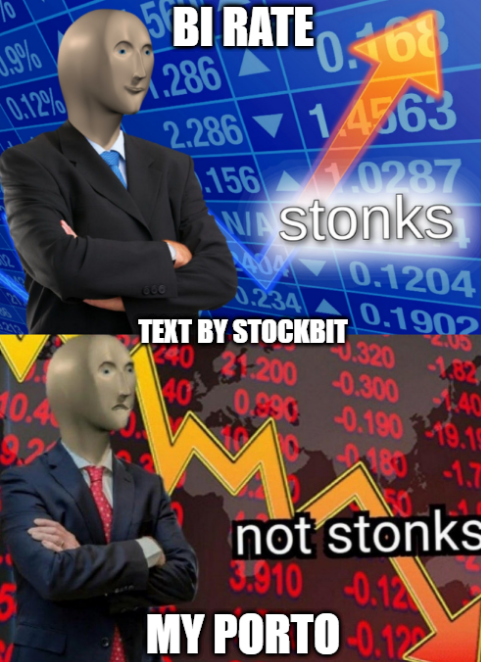
\includegraphics[width=0.50\textwidth]{cover.png}\par

	\vspace{0.6cm}
	{\Large\bfseries Disusun oleh:\par}
	\vspace{0.2cm}
	\textbf{\large Three Agents} \\
	\vspace{0.3cm}
	{\large
		\begin{tabular}{@{}p{6cm}r@{}}
			Muhammad Aufar Rizqi Kusuma & (13524061) \\
			Arina Azka                  & (13524049) \\
			Michael James Liman         & (13524106)
		\end{tabular}\par}

	\vspace{2.3cm}
	\large Laboratorium Intelegensi Buatan\\
	Program Studi Teknik Informatika\\
	Sekolah Teknik Elektro dan Informatika\\
	Institut Teknologi Bandung\\

\end{titlepage}

\hypersetup{pageanchor=true}
\clearpage
\pagestyle{fancy}

\tableofcontents
\clearpage

\chapter{Pendahuluan}
\section{Pengantar Permasalahan}
\section{Tujuan Permasalahan}
\section{Kerangka Teoretis Model Makroekonomi}



\chapter{Landasan Teori}
\section{Algoritma Hill Climbing}

Hill Climbing adalah algoritma pencarian lokal yang berusaha meningkatkan kualitas satu solusi secara bertahap. Algoritma memulai pencarian dari satu konfigurasi, membentuk sejumlah konfigurasi tetangga, lalu berpindah ke tetangga yang memberikan nilai objektif lebih baik. Pencarian berhenti saat tidak ditemukan tetangga yang meningkatkan nilai tersebut. Varian \textit{steepest-ascent} yang digunakan pada pseudocode memilih tetangga dengan nilai objektif tertinggi dari semua kandidat yang diperiksa \cite{poole2017artificial,russell2021artificial}.

Karakteristik utama Hill Climbing adalah penggunaan satu konfigurasi aktif dan keputusan yang hanya bergantung pada nilai konfigurasi tetangganya. Algoritma ini tidak menyimpan pohon pencarian atau seluruh jalur yang ditempuh. Karena setiap langkah memilih perbaikan lokal, nilai objektif konfigurasi yang dikunjungi meningkat secara monoton pada varian \textit{steepest-ascent} dengan perpindahan yang hanya menerima peningkatan ketat. Dengan ruang solusi berhingga, proses tersebut berakhir pada konfigurasi yang tidak memiliki tetangga lebih baik, yaitu optimum lokal \cite{poole2017artificial}.

Keunggulan Hill Climbing terletak pada kesederhanaan implementasi dan kebutuhan memori yang rendah dibandingkan metode yang menyimpan banyak kandidat pencarian. Algoritma ini juga dapat menghasilkan perbaikan dengan cepat apabila fungsi objektif dan pembentukan tetangga dapat dihitung secara efisien. Namun, hasilnya bergantung pada konfigurasi awal dan definisi tetangga. Pencarian dapat berhenti pada optimum lokal yang bukan optimum global, atau kesulitan bergerak pada daerah datar dan punggung sempit pada lanskap objektif. Oleh sebab itu, Hill Climbing tidak menjamin solusi terbaik secara global \cite{poole2017artificial,russell2021artificial}.

Hill Climbing sesuai digunakan ketika ruang solusi besar, evaluasi kualitas solusi relatif murah, dan solusi yang baik sudah berguna meskipun belum terbukti optimal. Metode ini kurang sesuai apabila dibutuhkan jaminan optimum global atau apabila perpindahan lokal jarang menghasilkan arah perbaikan yang informatif. Penggunaan beberapa titik awal atau varian yang mengizinkan langkah menyamping dapat mengurangi sebagian risiko terjebak, tetapi tidak mengubah sifat dasar metode pencarian lokal.

Dalam persoalan pemuatan paket, konfigurasi awal dibentuk secara acak sesuai spesifikasi. Algoritma kemudian membandingkan konfigurasi tetangga yang diperoleh melalui langkah perubahan susunan paket yang diizinkan, lalu memilih konfigurasi layak dengan nilai total paket yang lebih tinggi. Proses berlanjut sampai tidak ada tetangga yang meningkatkan nilai objektif. Pseudocode berikut menunjukkan varian \textit{steepest-ascent} tanpa langkah menyamping atau pengulangan dari titik awal baru.

\begingroup
\setlength{\parskip}{0pt}
\begin{list}{}{\setlength{\leftmargin}{0.1\linewidth}\setlength{\rightmargin}{0.1\linewidth}\setlength{\labelsep}{0pt}\setlength{\topsep}{0pt}\setlength{\partopsep}{0pt}\setlength{\parsep}{0pt}\setlength{\itemsep}{0pt}}\item[]
\noindent\rule{\linewidth}{0.8pt}\par\vspace{1pt}
\noindent\refstepcounter{algorithm}\textbf{Algorithm \thealgorithm:} Steepest-Ascent Hill Climbing\label{alg:steepest-ascent-hill-climbing}\par
\vspace{1pt}\noindent\rule{\linewidth}{0.4pt}\par\vspace{1pt}
\begin{algorithmic}
\REQUIRE Konfigurasi awal $s_0$, fungsi tetangga $N$, fungsi objektif $f$
\ENSURE Konfigurasi optimum lokal $s$
\STATE $s \gets s_0$
\WHILE{$N(s) \neq \emptyset$}
    \STATE $s' \gets \arg\max_{u \in N(s)} f(u)$
    \IF{$f(s') \leq f(s)$}
        \RETURN $s$
    \ENDIF
    \STATE $s \gets s'$
\ENDWHILE
\RETURN $s$
\end{algorithmic}
\par\vspace{1pt}\noindent\rule{\linewidth}{0.8pt}
\end{list}
\endgroup

\section{Algoritma Simulated Annealing}

Simulated Annealing adalah algoritma pencarian lokal stokastik yang meniru proses pendinginan material untuk mencari solusi bernilai objektif tinggi. Berbeda dari Hill Climbing yang hanya menerima perpindahan ke solusi lebih baik, Simulated Annealing juga dapat menerima solusi yang lebih buruk dengan peluang tertentu. Mekanisme ini membantu pencarian keluar dari optimum lokal dan mengeksplorasi bagian lain dari ruang solusi \cite{russell2021artificial,kirkpatrick1983optimization}.

Pada setiap iterasi, algoritma memilih satu solusi tetangga dan menghitung perubahan nilai objektifnya. Untuk persoalan maksimisasi, perubahan tersebut didefinisikan sebagai $\Delta E=f(s')-f(s)$, dengan $s$ sebagai solusi saat ini dan $s'$ sebagai kandidat tetangga. Kandidat yang meningkatkan atau mempertahankan nilai objektif selalu diterima. Kandidat yang menurunkan nilai objektif dapat diterima dengan peluang yang bergantung pada temperatur $T$, seperti dirumuskan pada Persamaan~\ref{eq:sa-acceptance} \cite{kirkpatrick1983optimization}.

\begin{equation}
P(\text{menerima } s') =
\begin{cases}
1, & \Delta E \geq 0, \\
\exp\left(\dfrac{\Delta E}{T}\right), & \Delta E < 0.
\end{cases}
\label{eq:sa-acceptance}
\end{equation}

Temperatur mengendalikan tingkat eksplorasi algoritma. Pada temperatur tinggi, penurunan nilai objektif masih mungkin diterima sehingga pencarian dapat menjelajahi ruang solusi dengan lebih luas. Ketika temperatur diturunkan, peluang menerima perpindahan yang lebih buruk ikut mengecil dan pencarian semakin berfokus pada perbaikan. Salah satu jadwal pendinginan yang umum digunakan adalah pendinginan geometris, dengan $0<\alpha<1$ sebagai faktor pendinginan \cite{russell2021artificial}.

\begin{equation}
T_{k+1}=\alpha T_k, \qquad 0<\alpha<1.
\label{eq:sa-cooling}
\end{equation}

Keunggulan Simulated Annealing adalah kemampuannya melewati optimum lokal dengan menerima perpindahan yang sesaat menurunkan nilai objektif, tanpa harus menyimpan banyak kandidat solusi. Namun, kualitas hasil dan waktu pencarian sensitif terhadap temperatur awal, faktor pendinginan, temperatur minimum, serta mekanisme pembentukan tetangga. Jika temperatur turun terlalu cepat, pencarian masih dapat terjebak pada optimum lokal; frekuensi kondisi ini menjadi salah satu metrik evaluasi algoritma. Karena itu, algoritma ini tidak menjamin solusi global terbaik untuk jadwal pendinginan berdurasi terbatas dan hasilnya dapat berbeda antarpercobaan \cite{russell2021artificial,kirkpatrick1983optimization}.

Simulated Annealing cocok digunakan pada ruang solusi besar dengan banyak optimum lokal, terutama ketika evaluasi solusi cukup murah dan solusi mendekati optimal sudah bermanfaat. Dalam persoalan pemuatan paket, pencarian dimulai dari konfigurasi acak. Pada setiap iterasi, satu tetangga dibentuk melalui operasi pertukaran paket, pemindahan paket, atau rotasi. Algoritma menerima kandidat yang meningkatkan nilai objektif, dan sesekali menerima kandidat yang menurunkannya sesuai peluang pada Persamaan~\ref{eq:sa-acceptance}. Temperatur kemudian dikurangi berdasarkan jadwal pendinginan. Nilai $\exp(\Delta E/T)$ menjadi ukuran peluang penerimaan kandidat yang lebih buruk, sesuai metrik yang diminta spesifikasi untuk dianalisis terhadap iterasi.

Pseudocode berikut menggunakan pendinginan geometris dan berhenti ketika temperatur mencapai nilai minimum. Variabel $s_{\text{best}}$ menyimpan konfigurasi bernilai tertinggi yang ditemukan, meskipun proses menerima perpindahan sementara ke konfigurasi yang lebih buruk.

\begingroup
\setlength{\parskip}{0pt}
\begin{list}{}{\setlength{\leftmargin}{0.1\linewidth}\setlength{\rightmargin}{0.1\linewidth}\setlength{\labelsep}{0pt}\setlength{\topsep}{0pt}\setlength{\partopsep}{0pt}\setlength{\parsep}{0pt}\setlength{\itemsep}{0pt}}\item[]
\noindent\rule{\linewidth}{0.8pt}\par\vspace{1pt}
\noindent\refstepcounter{algorithm}\textbf{Algorithm \thealgorithm:} Simulated Annealing\label{alg:simulated-annealing}\par
\vspace{1pt}\noindent\rule{\linewidth}{0.4pt}\par\vspace{1pt}
\begin{algorithmic}
\REQUIRE Solusi awal $s_0$, fungsi tetangga $N$, fungsi objektif $f$, parameter $T_0>T_{\min}>0$ dan $0<\alpha<1$
\ENSURE Solusi terbaik yang ditemukan $s_{\text{best}}$
\STATE $s \gets s_0$, $s_{\text{best}} \gets s_0$, $T \gets T_0$
\WHILE{$T > T_{\min}$}
    \IF{$N(s) = \emptyset$}
        \RETURN $s_{\text{best}}$
    \ENDIF
    \STATE Pilih $s'$ secara acak dari $N(s)$
    \STATE $\Delta E \gets f(s') - f(s)$
    \IF{$\Delta E \geq 0$}
        \STATE $s \gets s'$
    \ELSE
        \STATE Bangkitkan $u$ secara acak dari $[0,1]$
        \IF{$u < \exp(\Delta E/T)$}
            \STATE $s \gets s'$
        \ENDIF
    \ENDIF
    \IF{$f(s) > f(s_{\text{best}})$}
        \STATE $s_{\text{best}} \gets s$
    \ENDIF
    \STATE $T \gets \alpha T$
\ENDWHILE
\RETURN $s_{\text{best}}$
\end{algorithmic}
\par\vspace{1pt}\noindent\rule{\linewidth}{0.8pt}
\end{list}
\endgroup

\section{Genetic Algorithm}

Genetic Algorithm adalah metode pencarian berbasis populasi yang memperbarui kumpulan kandidat solusi melalui mekanisme yang terinspirasi oleh seleksi alam. Setiap kandidat disebut individu, sedangkan nilai objektifnya berperan sebagai ukuran fitness. Pada tiap generasi, algoritma memilih individu sebagai induk, menggabungkan bagian solusi melalui crossover, lalu menerapkan mutasi secara acak untuk membentuk populasi baru \cite{russell2021artificial,goldberg1989genetic}.

Karakteristik Genetic Algorithm adalah pencarian atas banyak kandidat secara bersamaan dan penggunaan operator stokastik untuk menghasilkan generasi berikutnya. Seleksi roulette memberi peluang lebih besar kepada individu dengan fitness lebih tinggi. Jika fitness individu ke-$i$ adalah $f_i$ dan bobot seleksinya $w_i$, peluang memilih individu tersebut dirumuskan sebagai

\begin{equation}
P(i)=\frac{w_i}{\sum_{j=1}^{n} w_j}.
\label{eq:ga-selection}
\end{equation}

Untuk persoalan pemuatan paket dengan nilai objektif nonnegatif, bobot seleksi dapat menggunakan nilai objektif. Jika seluruh bobot bernilai nol, seleksi dilakukan secara seragam. Crossover satu titik menggabungkan gen dari dua induk, sementara mutasi mengubah satu gen dengan peluang tertentu. Kedua operator harus menghasilkan individu yang memenuhi batasan pemuatan paket \cite{goldberg1989genetic}.

Keunggulan Genetic Algorithm adalah kemampuannya mengeksplorasi beberapa wilayah ruang solusi secara paralel dan mengurangi ketergantungan pencarian pada satu konfigurasi awal. Keragaman populasi dapat membantu pencarian menghindari optimum lokal. Namun, hasil dan waktu pencarian bergantung pada ukuran populasi, jumlah generasi, operator, serta parameter seperti laju mutasi. Algoritma ini tidak menjamin solusi global terbaik dalam jumlah generasi terbatas, dan setiap generasi memerlukan evaluasi banyak kandidat \cite{russell2021artificial,goldberg1989genetic}.

Genetic Algorithm sesuai untuk ruang solusi besar dengan representasi kandidat yang dapat digabungkan dan dimutasi, khususnya ketika solusi layak dapat dipulihkan setelah operator diterapkan. Pada persoalan pemuatan paket, satu individu merepresentasikan penempatan seluruh paket. Populasi awal memuat konfigurasi awal yang valid dan konfigurasi valid lain yang dibentuk secara acak. Di setiap generasi, individu dievaluasi dengan fungsi objektif, induk dipilih menggunakan roulette, kemudian crossover satu titik dan mutasi dilakukan untuk membentuk populasi berikutnya. Individu terbaik disimpan terpisah sepanjang pencarian agar solusi terbaik tetap tersedia meskipun tidak diwariskan ke generasi baru.

Pseudocode berikut menggunakan seleksi roulette, crossover satu titik dengan perbaikan kelayakan, dan mutasi satu gen dengan peluang $\mu$. Pencarian berhenti setelah jumlah generasi yang ditentukan dan mengembalikan individu terbaik yang pernah dievaluasi.

\begingroup
\setlength{\parskip}{0pt}
\begin{list}{}{\setlength{\leftmargin}{0.1\linewidth}\setlength{\rightmargin}{0.1\linewidth}\setlength{\labelsep}{0pt}\setlength{\topsep}{0pt}\setlength{\partopsep}{0pt}\setlength{\parsep}{0pt}\setlength{\itemsep}{0pt}}\item[]
\noindent\rule{\linewidth}{0.8pt}\par\vspace{1pt}
\noindent\refstepcounter{algorithm}\textbf{Algorithm \thealgorithm:} Genetic Algorithm\label{alg:genetic-algorithm}\par
\vspace{1pt}\noindent\rule{\linewidth}{0.4pt}\par\vspace{1pt}
\begin{algorithmic}
\REQUIRE Solusi awal valid $s_0$, fungsi objektif $f$, ukuran populasi $n$, jumlah generasi $G$, laju mutasi $\mu$
\ENSURE Individu terbaik yang ditemukan $s_{\text{best}}$
\STATE $P \gets$ populasi valid berukuran $n$ yang memuat $s_0$
\STATE $s_{\text{best}} \gets s_0$, $f_{\text{best}} \gets -\infty$
\FOR{$g \gets 0$ sampai $G$}
    \STATE Evaluasi $f(x)$ untuk setiap $x \in P$
    \STATE $x_{\text{best}} \gets \arg\max_{x \in P} f(x)$
    \IF{$f(x_{\text{best}}) > f_{\text{best}}$}
        \STATE $s_{\text{best}} \gets x_{\text{best}}$, $f_{\text{best}} \gets f(x_{\text{best}})$
    \ENDIF
    \IF{$g < G$}
        \STATE $P_{\text{baru}} \gets \emptyset$
        \WHILE{$|P_{\text{baru}}| < n$}
            \STATE Pilih induk $p_1$ dan $p_2$ dari $P$ dengan seleksi roulette
            \STATE $c \gets$ crossover satu titik $(p_1,p_2)$ dan perbaiki agar valid
            \STATE Dengan peluang $\mu$, mutasikan satu gen pada $c$ dan pertahankan validitasnya
            \STATE Tambahkan $c$ ke $P_{\text{baru}}$
        \ENDWHILE
        \STATE $P \gets P_{\text{baru}}$
    \ENDIF
\ENDFOR
\RETURN $s_{\text{best}}$
\end{algorithmic}
\par\vspace{1pt}\noindent\rule{\linewidth}{0.8pt}
\end{list}
\endgroup


\chapter{Implementasi Algoritma}
\section{Representasi State}

\section{\textit{Constraint} Permasalahan}

\section{\textit{Succesor Function}}

\section{\textit{Objective Function}}

\section{Formulasi \textit{Initial State}}

\section{Implementasi Hill Climbing}

Seluruh varian \textit{hill climbing} diimplementasikan pada berkas \texttt{src/\allowbreak algorithms/\allowbreak hill\_\allowbreak climbing/\allowbreak algorithm.py} di atas representasi \textit{state}, validator \textit{constraint}, dan fungsi \textit{neighbor} yang sama dengan algoritma lainnya (\texttt{State}, \texttt{validate\_state}, dan \texttt{random\_neighbor}). Dengan demikian seluruh algoritma menerima masukan dan mengembalikan keluaran yang seragam, yaitu objek \texttt{SearchResult} yang memuat \textit{state} awal, \textit{state} akhir, nilai \textit{objective function} akhir, riwayat nilai per iterasi, durasi pencarian, dan metrik khusus algoritma.

\subsection{Pembangkitan \textit{Neighbor} dan Heuristik}
Ruang \textit{neighbor} pada permasalahan ini sangat besar karena koordinat paket berupa bilangan bulat, sehingga seluruh \textit{neighbor} tidak dapat dienumerasi pada setiap iterasi. Sebagai gantinya, setiap \textit{neighbor} dibangkitkan oleh \texttt{random\_neighbor}, yang secara acak memilih salah satu dari tiga operasi (menukar dua paket, memindahkan paket ke koordinat lain, atau merotasi paket $90^{\circ}$) dan hanya mengembalikan \textit{state} yang lolos validasi \textit{constraint}.

Heuristik yang kami gunakan adalah \textit{steepest} berbasis sampel: pada setiap iterasi dibangkitkan \texttt{neighbors\_per\_iteration} (bawaan 30) \textit{neighbor} valid, kemudian \textit{neighbor} dengan nilai terbaik dianggap sebagai \textit{neighbor} terbaik. Konsekuensinya, varian \textit{steepest} dan \textit{sideways} tidak menjamin menemukan \textit{neighbor} terbaik yang sesungguhnya, tetapi peluangnya naik seiring bertambahnya ukuran sampel. Varian \textit{stochastic} memakai tepat satu \textit{neighbor} per iterasi.

\subsection{Parameter dan Kondisi Berhenti}
\begin{table}[h]
    \centering
    \begin{tabular}{@{}p{4.7cm}p{2.3cm}p{6.5cm}@{}}
        \toprule
        Parameter                          & Bawaan            & Keterangan                                                                                           \\
        \midrule
        \texttt{variant}                   & \texttt{steepest} & \texttt{steepest}, \texttt{sideways}, \texttt{stochastic}, atau \texttt{random\_restart}             \\
        \texttt{neighbors\_per\_iteration} & 30                & Jumlah \textit{neighbor} yang disampel per iterasi (tidak dipakai \textit{stochastic})               \\
        \texttt{max\_iterations}           & 1000              & Batas iterasi; menjadi kondisi berhenti pada \textit{stochastic} dan batas pengaman pada varian lain \\
        \texttt{max\_sideways}             & 100               & Batas \textit{sideways move} (varian \textit{sideways})                                              \\
        \texttt{max\_restarts}             & 10                & Jumlah \textit{restart} setelah percobaan pertama (varian \textit{random restart})                   \\
        \texttt{seed}                      & ---               & Seed pembangkit acak agar eksperimen dapat diulang                                                   \\
        \bottomrule
    \end{tabular}
    \caption{Parameter algoritma \textit{hill climbing}}
\end{table}

\begin{itemize}
    \item \textit{Steepest}: berhenti ketika \textit{neighbor} terbaik dari sampel tidak lebih baik daripada \textit{state} saat ini.
    \item \textit{Sideways}: sama seperti \textit{steepest}, tetapi \textit{neighbor} bernilai sama diterima selama jumlah \textit{sideways move} belum mencapai \texttt{max\_sideways}.
    \item \textit{Stochastic}: berhenti setelah \texttt{max\_iterations} iterasi. Iterasi yang \textit{neighbor}-nya ditolak tetap dihitung.
    \item \textit{Random restart}: menjalankan \textit{steepest} dari \textit{state} awal yang diberikan, lalu dari \texttt{max\_restarts} \textit{state} acak baru, sehingga total terdapat \texttt{max\_restarts}\,+\,1 pendakian. Hasil terbaik dari seluruh pendakian dikembalikan.
\end{itemize}

\subsection{Metrik yang Dicatat}
Setiap \textit{run} mengembalikan \texttt{HillClimbingMetrics} yang berisi varian yang dipakai, banyak iterasi hingga berhenti, jumlah dan batas \textit{sideways move}, jumlah dan batas \textit{restart}, serta banyak iterasi pada setiap \textit{restart}. Riwayat nilai \textit{objective function} dicatat pada setiap iterasi (elemen pertama adalah nilai \textit{state} awal) dan digunakan untuk membuat plot nilai \textit{objective function} terhadap banyak iterasi. Durasi pencarian diukur dengan \texttt{perf\_counter}.

\subsection{\textit{Source Code}}
Fungsi \texttt{\_climb} menjalankan satu pendakian untuk varian \textit{steepest}, \textit{sideways}, atau \textit{stochastic}. Fungsi \texttt{hill\_climbing} memvalidasi parameter, memilih varian, menangani pengulangan pada \textit{random restart}, lalu menyusun \texttt{SearchResult}.

\begin{lstlisting}[language=Python, caption={Fungsi bantu dan \texttt{\_climb} pada \texttt{algorithm.py}}]
from math import isfinite
from random import Random
from time import perf_counter

from src.contracts import ObjectiveFunction, resolve_objective
from src.model import State
from src.neighbors import random_initial_state, random_neighbor
from src.results import HillClimbingMetrics, ObjectiveValue, SearchResult

VARIANTS = ("steepest", "sideways", "stochastic", "random_restart")


def _check_int(value, name: str, minimum: int) -> None:
    if type(value) is not int or value < minimum:
        raise ValueError(f"{name} must be an integer >= {minimum}")


def _score(objective: ObjectiveFunction[State], state: State) -> ObjectiveValue:
    score = objective(state)
    if isinstance(score, bool) or not isinstance(score, (int, float)) or not isfinite(score):
        raise ValueError("objective_fn must return finite integer or float values")
    return score


def _climb(
    start: State,
    objective: ObjectiveFunction[State],
    rng: Random,
    *,
    variant: str,
    neighbors_per_iteration: int,
    max_iterations: int,
    max_sideways: int,
) -> tuple[State, ObjectiveValue, list[ObjectiveValue], int, int]:
    """One climb. Returns (state, score, history, iterations, sideways_moves).

    history[0] is the start score; one entry is appended per iteration.
    """
    current, current_score = start, _score(objective, start)
    history = [current_score]
    iterations = sideways = 0

    while iterations < max_iterations:
        if variant == "stochastic":
            candidates = [random_neighbor(current, rng)]
        else:
            candidates = [random_neighbor(current, rng) for _ in range(neighbors_per_iteration)]
        scored = [(_score(objective, c), c) for c in candidates]
        best_score, best = max(scored, key=lambda pair: pair[0])

        if best_score > current_score:
            current, current_score = best, best_score
        elif variant == "sideways" and best_score == current_score and sideways < max_sideways:
            current = best
            sideways += 1
        elif variant == "stochastic":
            iterations += 1  # a rejected random neighbor still costs an iteration
            history.append(current_score)
            continue
        else:
            break  # local optimum (or sideways budget exhausted)
        iterations += 1
        history.append(current_score)

    return current, current_score, history, iterations, sideways
\end{lstlisting}

\begin{lstlisting}[language=Python, caption={Fungsi \texttt{hill\_climbing} pada \texttt{algorithm.py}}]
def hill_climbing(
    initial_state: State,
    *,
    seed: int,
    objective_fn: ObjectiveFunction[State] | None = None,
    variant: str = "steepest",
    neighbors_per_iteration: int = 30,
    max_iterations: int = 1000,
    max_sideways: int = 100,
    max_restarts: int = 10,
    objective_name: str | None = None,
    run_index: int = 1,
) -> SearchResult[State]:
    """Run one hill-climbing variant and return a shared-contract SearchResult."""
    if variant not in VARIANTS:
        raise ValueError(f"variant must be one of {VARIANTS}")
    if type(seed) is not int:
        raise ValueError("seed must be an integer")
    _check_int(neighbors_per_iteration, "neighbors_per_iteration", 1)
    _check_int(max_iterations, "max_iterations", 0)
    _check_int(max_sideways, "max_sideways", 0)
    _check_int(max_restarts, "max_restarts", 0)
    _check_int(run_index, "run_index", 1)

    started_at = perf_counter()
    rng = Random(seed)
    objective = resolve_objective(initial_state, objective_fn)
    climb_kwargs = dict(
        variant="steepest" if variant == "random_restart" else variant,
        neighbors_per_iteration=neighbors_per_iteration,
        max_iterations=max_iterations,
        max_sideways=max_sideways,
    )

    if variant == "random_restart":
        # Restart 0 uses the supplied initial state; each later one a fresh random state.
        best_state, best_score = initial_state, None
        history: list[ObjectiveValue] = []
        per_restart: list[int] = []
        for restart in range(max_restarts + 1):
            start = (
                initial_state
                if restart == 0
                else random_initial_state(initial_state.packages, initial_state.truck, rng)
            )
            state, score, hist, iters, _ = _climb(start, objective, rng, **climb_kwargs)
            history.extend(hist)
            per_restart.append(iters)
            if best_score is None or score > best_score:
                best_state, best_score = state, score
        final_state, final_score = best_state, best_score
        iterations, sideways = sum(per_restart), 0
        restarts = max_restarts
    else:
        final_state, final_score, history, iterations, sideways = _climb(
            initial_state, objective, rng, **climb_kwargs
        )
        per_restart, restarts = [], 0

    parameters: dict[str, int | float | str | bool] = {
        "variant": variant,
        "max_iterations": max_iterations,
    }
    if variant != "stochastic":
        parameters["neighbors_per_iteration"] = neighbors_per_iteration
    if variant == "sideways":
        parameters["max_sideways"] = max_sideways
    if variant == "random_restart":
        parameters["max_restarts"] = max_restarts

    return SearchResult(
        algorithm=f"hill_climbing_{variant}",
        objective_name=objective_name or ("total_value" if objective_fn is None else "custom"),
        initial_state=initial_state,
        final_state=final_state,
        objective_value=final_score,
        objective_history=tuple(history),
        duration_seconds=perf_counter() - started_at,
        metrics=HillClimbingMetrics(
            variant=variant,
            iterations=iterations,
            sideways_moves=sideways,
            maximum_sideways_moves=max_sideways if variant == "sideways" else None,
            restarts=restarts,
            maximum_restarts=max_restarts if variant == "random_restart" else None,
            iterations_per_restart=tuple(per_restart),
        ),
        seed=seed,
        run_index=run_index,
        parameters=parameters,
    )
\end{lstlisting}

\begin{lstlisting}[language=Python, caption={Fungsi pembungkus tiap varian pada \texttt{algorithm.py}}]
def steepest_ascent_hill_climbing(initial_state: State, **kw) -> SearchResult[State]:
    return hill_climbing(initial_state, variant="steepest", **kw)


def sideways_hill_climbing(initial_state: State, **kw) -> SearchResult[State]:
    return hill_climbing(initial_state, variant="sideways", **kw)


def stochastic_hill_climbing(initial_state: State, **kw) -> SearchResult[State]:
    return hill_climbing(initial_state, variant="stochastic", **kw)


def random_restart_hill_climbing(initial_state: State, **kw) -> SearchResult[State]:
    return hill_climbing(initial_state, variant="random_restart", **kw)
\end{lstlisting}

\subsection{Pelaksana Eksperimen dan Visualisasi}
Berkas \texttt{src/\allowbreak experiments/\allowbreak hill\_\allowbreak climbing.py} menjalankan setiap varian sebanyak tiga kali dengan tiga \textit{seed} berbeda. \textit{State} awal setiap \textit{run} dibangkitkan secara acak dari \textit{seed} tersebut. Untuk setiap \textit{run}, program menyimpan berkas \texttt{result.json}, plot nilai \textit{objective function} terhadap iterasi, dan visualisasi tiga dimensi \textit{state} awal dan akhir. Ringkasan lintas \textit{run} (rata-rata dan simpangan baku nilai akhir, durasi, dan iterasi) disimpan pada \texttt{summary.json} dan \texttt{summary.png}. Program dijalankan melalui \texttt{src/\allowbreak experiments/\allowbreak run\_\allowbreak hill\_\allowbreak climbing.py}.

\section{Implementasi Simullated Annealing}

\section{Implementasi Genetic Algorithm}





\chapter{Hasil Eksperimen dan Analisis}
\section{Metodologi Eksperimen}

Metodologi eksperimen dirancang untuk membandingkan kualitas solusi dan biaya pencarian secara adil, sekaligus memeriksa ketahanan algoritma pada kasus sulit dan masukan batas. Seluruh algoritma diuji pada instance paket dan truk yang sama, menggunakan fungsi objektif serta validator constraint yang sama. Rincian konfigurasi khusus tiap algoritma dibahas terpisah dan tidak diulang pada metodologi umum ini.

\subsection{Kumpulan Instance dan Kasus Uji}

Kumpulan uji mencakup instance dasar sintetis karena spesifikasi tugas tidak menyediakan data paket. Instance terkontrol diturunkan dari kasus dasar untuk menguji karakteristik tertentu. Ukuran dan tingkat kesulitan dibuat bervariasi agar hasil mewakili beberapa konfigurasi pemuatan. Pengujian mencakup kategori berikut.

\begin{enumerate}
    \renewcommand{\labelenumi}{(\arabic{enumi})}
    \item \textbf{Kasus dasar.} Instance dengan paket yang bervariasi dalam dimensi, nilai, dan berat, serta beberapa kombinasi pemuatan yang layak. Kasus ini digunakan untuk membandingkan kinerja umum.
    \item \textbf{Kasus kendala ketat.} Ruang truk diperkecil atau kapasitas berat dikurangi agar lebih banyak kandidat penempatan ditolak. Instance ini menguji dampak keterbatasan ruang dan kapasitas.
    \item \textbf{Kasus tanpa pemuatan nonkosong yang layak.} Semua paket dibuat tidak dapat dimuat, misalnya setiap paket lebih besar daripada ruang truk pada semua orientasi atau beratnya melebihi kapasitas. Karena representasi tetap mengizinkan semua paket berada di luar truk, state kosong merupakan state valid dengan nilai objektif nol. Kasus ini menguji apakah algoritma dapat mengembalikan state valid tanpa paket termuat.
    \item \textbf{Kasus batas dan struktur khusus.} Pengujian meliputi satu paket, paket yang hanya muat setelah rotasi, paket yang tepat menyentuh dinding truk, berat total yang tepat sama dengan kapasitas, paket rapuh yang memengaruhi dukungan, serta paket bernilai atau berbobot nol. Kasus dengan fitness sama juga digunakan untuk memeriksa perilaku ketika seleksi tidak memiliki preferensi nilai.
    \item \textbf{Masukan tidak valid.} Data dengan dimensi atau kapasitas yang melanggar format, ID paket duplikat, atau daftar paket kosong diuji pada batas validasi data. Kasus ini dipisahkan dari benchmark pencarian karena bukan instance masalah yang sah menurut loader.
\end{enumerate}

Instance sintetis untuk uji batas dibuat dengan mengubah satu karakteristik pada satu waktu dari instance dasar, sementara atribut lain dipertahankan. Dengan demikian, perbedaan hasil dapat dikaitkan dengan kendala yang sedang diuji. Kasus yang dirancang untuk memastikan tidak ada paket yang dapat dimuat dibedakan secara eksplisit dari kasus sulit yang masih memiliki solusi layak.

\subsection{Protokol Perbandingan}

Untuk setiap pasangan instance dan seed, state awal yang sama digunakan oleh semua algoritma. Daftar seed ditetapkan sebelum eksperimen. Setiap kombinasi dijalankan sedikitnya tiga kali dengan seed berbeda sesuai kebutuhan evaluasi tugas. Jika anggaran komputasi memungkinkan, jumlah pengulangan ditambah agar estimasi variasi hasil lebih stabil. Penggunaan seed dan state awal berpasangan mengurangi pengaruh variasi inisialisasi saat membandingkan metode.

Selain jenis instance, faktor lain seperti data paket, truk, fungsi objektif, dan implementasi validasi dijaga tetap sama. Batas penghentian dan konfigurasi spesifik mengikuti definisi masing-masing algoritma. Karena satu iterasi pada algoritma berbeda belum tentu setara, jumlah iterasi tidak digunakan sendirian sebagai ukuran biaya lintas algoritma. Durasi pencarian dan jumlah evaluasi fungsi objektif dicatat sebagai ukuran biaya yang lebih langsung. Pengukuran waktu dilakukan pada lingkungan komputasi yang sama, dengan waktu persiapan data dan pembuatan visualisasi dipisahkan dari waktu pencarian.

Setiap hasil akhir diperiksa kembali menggunakan validator. Run dinyatakan berhasil jika algoritma mengembalikan state valid. Pada instance tanpa pemuatan nonkosong yang layak, state akhir harus valid dan tidak memuat paket. State awal dan akhir, seed, nilai objektif, jumlah paket termuat, riwayat pencarian, durasi, serta konfigurasi run disimpan agar hasil dapat direproduksi dan ditelusuri.

\subsection{Metrik dan Analisis}

Kualitas hasil dinilai dari nilai objektif akhir dan jumlah paket yang termuat. Ketahanan terhadap constraint dinilai dari proporsi run yang menghasilkan state akhir valid. Konsistensi diukur dengan merangkum nilai objektif dan durasi antarrun menggunakan rata-rata serta simpangan baku. Hasil tiap run tetap disajikan agar variasi tidak tersembunyi oleh agregat. Riwayat nilai objektif juga ditampilkan untuk memperlihatkan perkembangan pencarian. Untuk perbandingan lintas algoritma, kurva dapat disejajarkan terhadap jumlah evaluasi objektif atau waktu berjalan, selain menampilkan sumbu iterasi atau generasi yang diwajibkan untuk masing-masing algoritma.

Pada kasus tanpa pemuatan nonkosong yang layak, nilai objektif nol saja tidak cukup untuk menyimpulkan perilaku algoritma karena paket bernilai nol dapat saja termuat. Oleh sebab itu, jumlah paket termuat dan validitas state diperiksa bersamaan dengan nilai objektif. Hasil kasus ini dilaporkan sebagai uji ketahanan, terpisah dari perbandingan kualitas solusi pada instance yang dapat dimuat.

\subsection{Studi Ablasi}

Studi ablasi digunakan untuk mengetahui kontribusi pilihan desain terhadap hasil pencarian. Untuk setiap studi, satu konfigurasi acuan dibandingkan dengan beberapa varian konfigurasi. Pada tiap perbandingan, hanya faktor yang sedang diuji yang diubah. Instance, state awal, seed, fungsi objektif, constraint, dan anggaran pencarian lainnya dijaga tetap sama. Jika dua faktor diduga saling memengaruhi, interaksinya diuji pada eksperimen terpisah, bukan diubah sekaligus tanpa kontrol.

Setiap varian dijalankan dengan seed dan state awal yang sama seperti konfigurasi acuan. Analisis membandingkan nilai objektif akhir dan durasi serta menyajikan rata-rata, simpangan baku, dan riwayat pencarian. Dengan demikian, studi ablasi menunjukkan apakah perubahan konfigurasi memberi hasil yang konsisten pada seed yang diuji.

\subsection{Dataset dan Konfigurasi Eksperimen}
Seluruh eksperimen dijalankan dengan representasi \textit{state}, validator \textit{constraint}, dan fungsi \textit{neighbor} yang sama untuk ketiga algoritma. Spesifikasi tugas tidak menyediakan data paket, sehingga seluruh \textit{instance} bersifat sintetis dan disimpan sebagai \textit{fixture} pada \texttt{tests/fixtures/}. Setiap kategori pada subbab pertama diwujudkan oleh satu atau lebih berkas, dan sifat tiap berkas diperiksa otomatis oleh \texttt{tests/test\_fixtures.py} (misalnya bahwa \texttt{tight-space} hanya berbeda dari \texttt{base} pada dimensi truk, atau bahwa tidak ada paket pada \texttt{infeasible} yang dapat dimuat sendirian).

\begin{table}[H]
    \centering
    \small
    \begin{tabular}{@{}p{2.6cm}p{3.3cm}p{1.0cm}p{2.3cm}p{5.4cm}@{}}
        \toprule
        Kategori                  & Berkas                              & Paket & Truk (kapasitas)          & Karakteristik                                                                                                                                           \\
        \midrule
        Dasar                     & \texttt{base.json}                  & 10    & $8\times6\times4$ (30)    & Dimensi, nilai, berat, ETA, dan kerapuhan bervariasi. Total berat 59 melebihi kapasitas sehingga harus dipilih himpunan bagian                          \\
        \midrule
        Kendala ketat             & \texttt{tight-space.json}           & 10    & $6\times4\times3$ (30)    & Paket dan kapasitas sama dengan \texttt{base}. Hanya dimensi truk diperkecil                                                                            \\
                                  & \texttt{tight-capacity.json}        & 10    & $8\times6\times4$ (15)    & Paket dan dimensi sama dengan \texttt{base}. Hanya kapasitas dikurangi                                                                                  \\
        \midrule
        Tanpa pemuatan layak      & \texttt{infeasible.json}            & 10    & $8\times6\times4$ (30)    & Perubahan dari \texttt{base}. Paket P01--P05 diberi satu sisi 9, melebihi sisi terpanjang truk. Paket P06--P10 diberi berat 31, melebihi kapasitas                          \\
        \midrule
        Batas dan struktur khusus & \texttt{boundary/single-package}    & 1     & $4\times4\times4$ (10)    & Satu paket yang muat                                                                                                                                    \\
                                  & \texttt{boundary/rotation-only}     & 2     & $5\times2\times2$ (10)    & Paket $2\times2\times5$ hanya muat setelah rotasi                                                                                                       \\
                                  & \texttt{boundary/wall-touching}     & 4     & $4\times4\times2$ (8)     & Empat paket $2\times2\times2$ mengisi truk tepat sampai dinding                                                                                         \\
                                  & \texttt{boundary/exact-capacity}    & 4     & $10\times10\times10$ (10) & Optimum (berat $4+3+3$) tepat sama dengan kapasitas                                                                                                     \\
                                  & \texttt{boundary/fragile-support}   & 3     & $2\times2\times2$ (10)    & Paket rapuh boleh berada di atas paket biasa, tetapi tidak boleh menopang                                                                               \\
                                  & \texttt{boundary/zero-value-weight} & 4     & $4\times4\times4$ (5)     & Paket bernilai nol, berbobot nol, dan keduanya nol                                                                                                      \\
                                  & \texttt{boundary/equal-fitness}     & 6     & $2\times2\times1$ (100)   & Enam paket identik. Seleksi tidak punya preferensi                                                                                                      \\
        \midrule
        Masukan tidak valid       & \texttt{invalid/} (8 berkas)        & ---   & ---                       & Dimensi paket tidak positif, terlalu panjang, atau bukan bilangan bulat. Dimensi truk tidak positif. Kapasitas negatif. ID ganda. Daftar paket kosong. Atribut hilang \\
        \bottomrule
    \end{tabular}
    \caption{\textit{Fixture} untuk tiap kategori kasus uji}
    \label{tab:fixtures}
\end{table}

Eksperimen memakai tiga fungsi objektif. \texttt{total\_value} adalah fungsi wajib. \texttt{eta\_weighted\_value} membagi nilai paket dengan $\text{ETA}+1$, sehingga paket yang mendesak mendapat bobot lebih besar. \texttt{compact\_value} menambahkan bonus kurang dari satu satuan untuk penataan yang lebih rendah. Pengujian dibagi menjadi empat rangkaian.

\begin{enumerate}
    \renewcommand{\labelenumi}{(\arabic{enumi})}
    \item \textbf{\textit{Benchmark} lintas kategori} (\texttt{src/experiments/run\_benchmark.py}). Seluruh algoritma pada seluruh \textit{fixture} valid dengan \texttt{total\_value}, lima \textit{seed} (11--15) dan satu konfigurasi parameter tetap, sehingga $11\ \text{instance} \times 5\ \textit{seed} \times 6\ \text{algoritma} = 330$ \textit{run}. Setiap \textit{run} mencatat validitas \textit{state} akhir, jumlah paket termuat, jumlah evaluasi objektif, dan durasi pencarian. Delapan \textit{fixture} tidak valid diberikan ke \textit{loader} data pada rangkaian yang sama.
    \item \textbf{Eksperimen per algoritma} pada \texttt{base} dengan tiga fungsi objektif dan tiga \textit{seed} (11--13), sesuai kebutuhan tugas. Pengujian mencakup empat varian \textit{hill climbing}, tiga \textit{run} SA, dan dua \textit{sweep} GA untuk generasi serta populasi. Perbandingan fungsi objektif juga diulang pada \texttt{tight-capacity} dengan konfigurasi yang sama.
    \item \textbf{Analisis GA lintas fixture dan parameter} dengan \texttt{total\_value}. Baseline dijalankan pada 11 fixture valid. Tiga \textit{sweep} satu faktor dilakukan pada \texttt{base} dengan lima \textit{seed} (11--15). Baseline memakai populasi 20 dan 40 generasi dengan laju mutasi 0,05. Nilai yang diuji untuk populasi adalah $\{10,20,40\}$, untuk generasi $\{20,40,80\}$, dan untuk laju mutasi $\{0 / 0{,}05 / 0{,}20\}$.
    \item \textbf{Studi ablasi GA} pada \texttt{base} dengan \texttt{total\_value} dan lima \textit{seed} (11--15).
\end{enumerate}

\begin{table}[H]
    \centering
    \begin{tabular}{@{}p{3.4cm}p{11.6cm}@{}}
        \toprule
        Algoritma                    & Parameter                                                                                                                                                                                                                                                                                              \\
        \midrule
        \textit{Hill climbing}       & Empat varian dengan \texttt{neighbors\_per\_iteration}\,=\,30, \texttt{max\_iterations}\,=\,1000, \texttt{max\_sideways}\,=\,100, dan \texttt{max\_restarts}\,=\,10                                                                                                                                                  \\
        \textit{Simulated annealing} & \texttt{max\_iterations}\,=\,3000, $T_0=100$, \texttt{cooling\_rate}\,=\,0,995, \texttt{stuck\_patience}\,=\,100                                                                                                                                                                                       \\
        \textit{Genetic algorithm}   & Baseline memakai populasi 20 dan 40 generasi dengan \textit{mutation rate} 0,05. \textit{Sweep} menguji populasi $\{10,20,40\}$, generasi $\{20,40,80\}$, serta laju mutasi $\{0 / 0{,}05 / 0{,}20\}$ dengan parameter lain tetap. Seleksi memakai \textit{roulette-wheel}. Ablasi memakai populasi 20 dan 50 generasi \\
        \bottomrule
    \end{tabular}
    \caption{Konfigurasi parameter eksperimen}
    \label{tab:konfigurasi}
\end{table}

\textit{State} awal setiap \textit{run} dibangkitkan secara acak dari \textit{seed} yang sama (\textit{seed} dikenai XOR dengan konstanta tetap), sehingga ketiga algoritma dan ketiga \textit{objective} memulai dari \textit{state} yang identik. Pada \texttt{base}, nilai total \textit{state} awal untuk \textit{seed} 11 sampai 15 berturut-turut adalah 330, 285, 320, 275, dan 275. Pada \texttt{tight-capacity} untuk \textit{seed} 11 sampai 13 adalah 155, 155, dan 160. Pada GA, \textit{state} awal menjadi anggota pertama populasi. Karena hanya ada tiga atau lima \textit{seed}, simpangan baku (simpangan baku sampel, dihitung ulang dari nilai tiap \textit{run}) harus dibaca sebagai gambaran sebaran kasar, bukan hasil uji statistik.

Nilai optimum sebagai acuan. Relaksasi yang hanya memperhatikan kapasitas berat (masalah \textit{knapsack}, dihitung dengan enumerasi) memberi batas atas 335 untuk \texttt{base} dan 175 untuk \texttt{tight-capacity}. Kedua batas ini tercapai oleh \textit{run} yang valid, sehingga 335 dan 175 adalah optimum sebenarnya. Pada \texttt{tight-space} batas atas yang sama (335) tidak tercapai oleh \textit{run} mana pun. Nilai terbaik yang ditemukan adalah 300, dan apakah itu optimum tidak diketahui. Pada tabel berikutnya, ``terbaik'' berarti nilai tertinggi yang ditemukan oleh seluruh \textit{run} pada \textit{instance} tersebut.

\section{Hasil Eksperimen dan Analisis tiap Algoritma}

Hasil \textit{hill climbing} dan SA pada bagian ini menggunakan \texttt{base} dengan tiga \textit{seed} (11--13), kecuali bila disebut lain. Protokol GA dijelaskan dan dilaporkan tersendiri karena mencakup seluruh kategori fixture serta lima seed (11--15).

\subsection{Hill Climbing}

\subsubsection{Fungsi objektif \texttt{total\_value}}
\begin{table}[H]
    \centering
    \begin{tabular}{@{}lrrrrr@{}}
        \toprule
        Varian                  & Rata-rata & Simpangan baku & Terbaik & Iterasi rata-rata & Durasi rata-rata (s) \\
        \midrule
        \textit{Steepest}       & 316,67    & 27,54          & 335     & 0,33              & 0,0053               \\
        \textit{Sideways}       & 318,33    & 28,87          & 335     & 100,67            & 0,4646               \\
        \textit{Stochastic}     & 318,33    & 24,66          & 335     & 1000              & 0,1703               \\
        \textit{Random restart} & 333,33    & 2,89           & 335     & 1,67              & 0,1535               \\
        \bottomrule
    \end{tabular}
    \caption{Hasil \textit{hill climbing} dengan \texttt{total\_value} (\texttt{base}, 3 \textit{seed})}
    \label{tab:hc-total}
\end{table}

Nilai akhir per \textit{seed} 11, 12, dan 13 untuk \textit{steepest} adalah 330, 285, dan 335. Nilai untuk \textit{sideways} adalah 335, 285, dan 335, untuk \textit{stochastic} adalah 330, 290, dan 335, sedangkan \textit{random restart} menghasilkan 335, 330, dan 335. \textit{Seed} 12 menjadi kasus tersulit. Nilai awalnya 285 dengan lima paket termuat dan merupakan \textit{local optimum} bagi \textit{steepest} serta \textit{sideways}. Varian pertama berhenti pada iterasi ke-0, sedangkan varian kedua memakai 100 \textit{sideways move} tanpa perbaikan. \textit{Stochastic} hanya mencapai 290 setelah 1000 iterasi. Pada \textit{seed} 11, \textit{steepest} dan \textit{stochastic} tidak memperbaiki nilai awal 330, sementara \textit{sideways} mencapai 335 melalui gerakan setara. Semua varian mencapai 335 pada \textit{seed} 13. Hasil ini menunjukkan bahwa gerakan tunggal \textit{swap}, \textit{move}, atau rotasi yang tidak boleh menurunkan nilai dapat membuat pencarian menetap pada optimum lokal.

\textit{Random restart} adalah satu-satunya varian yang tidak tersangkut pada \textit{seed} 12 (330) dan mencapai 335 pada dua \textit{seed} lain, sehingga simpangan bakunya turun dari sekitar 25--29 menjadi 2,89. Sepuluh pendakian tambahan dari \textit{state} acak memberi peluang untuk mendarat di cekungan yang berbeda. Iterasi rata-ratanya kecil (1,67) karena sebagian besar pendakian segera berhenti. Durasinya (0,15 detik) berada di antara \textit{steepest} dan \textit{sideways}.

\begin{figure}[H]
    \centering
    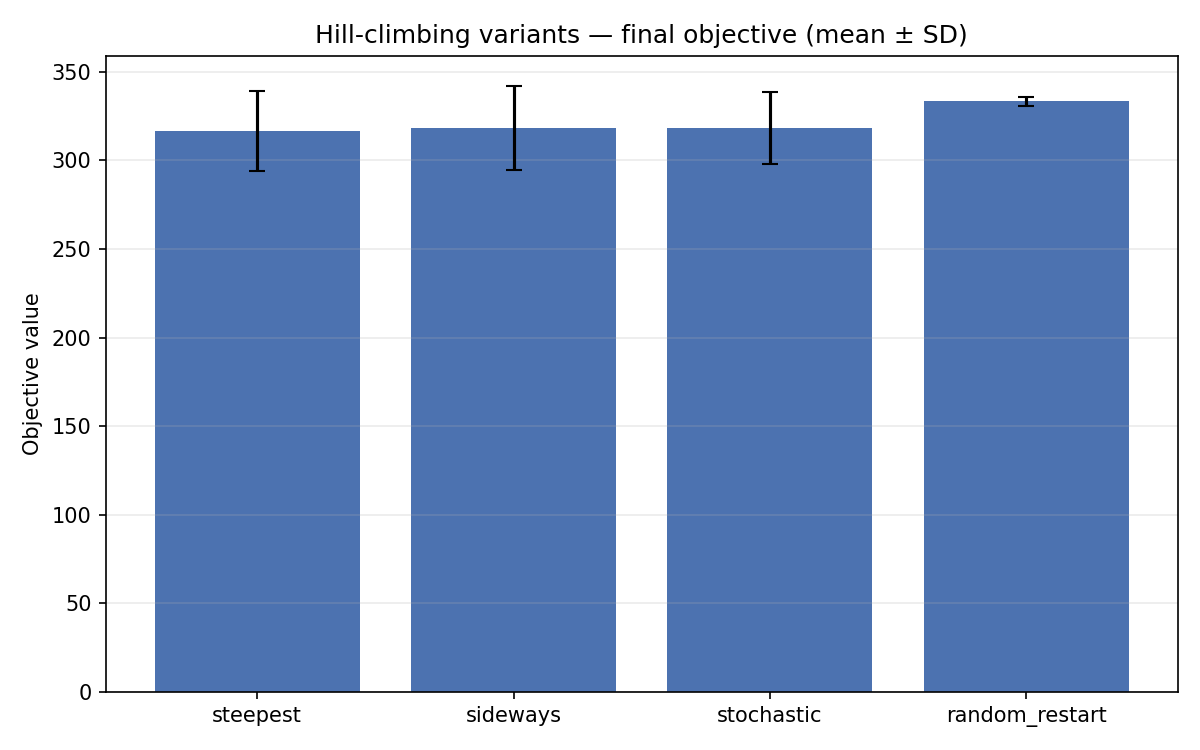
\includegraphics[width=0.78\textwidth]{figures/base/hc-summary-total_value.png}
    \caption{Ringkasan \textit{hill climbing} dengan \texttt{total\_value}}
\end{figure}

\begin{figure}[H]
    \centering
    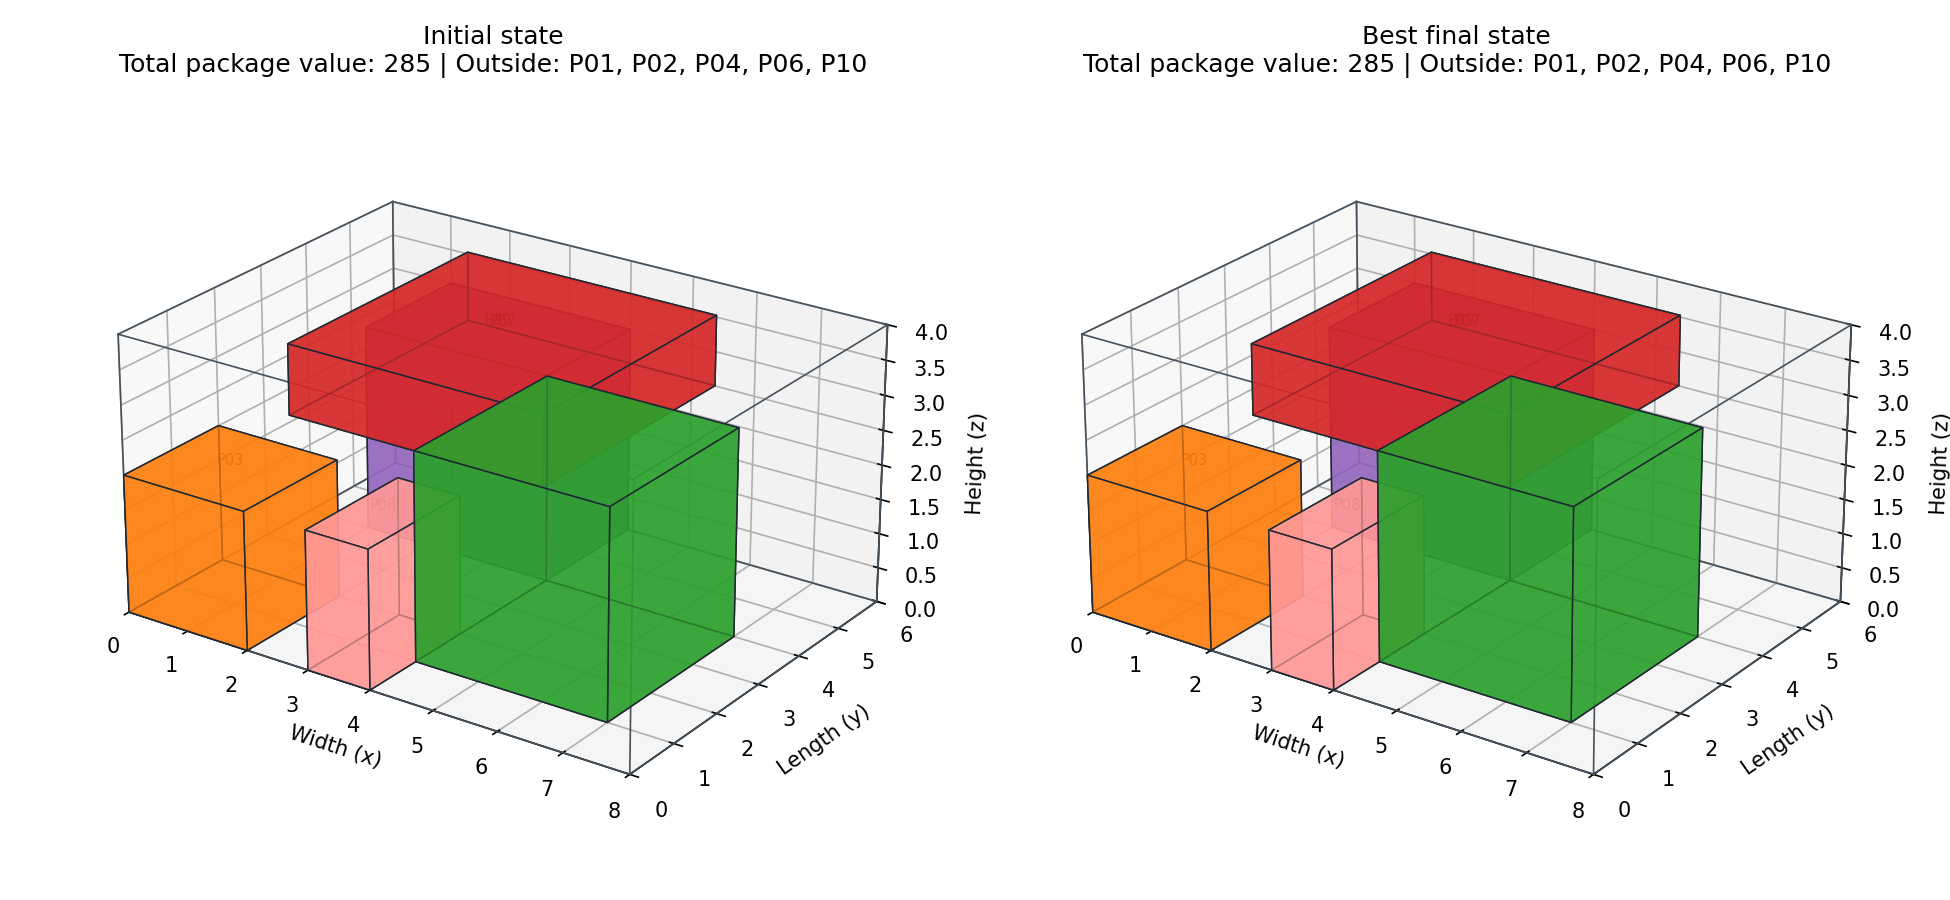
\includegraphics[width=0.85\textwidth]{figures/base/hc-states-steepest-seed12.png}
    \caption{\textit{State} awal dan akhir \textit{steepest} pada \textit{seed} 12. Kedua \textit{state} bernilai 285}
\end{figure}

\subsubsection{Fungsi objektif \texttt{eta\_weighted\_value}}
\begin{table}[H]
    \centering
    \begin{tabular}{@{}lrrrrr@{}}
        \toprule
        Varian                  & Rata-rata & Simpangan baku & Terbaik & Nilai total paket rata-rata & Durasi rata-rata (s) \\
        \midrule
        \textit{Steepest}       & 103,23    & 11,82          & 116,33  & 303,33                      & 0,0064               \\
        \textit{Sideways}       & 116,33    & 0              & 116,33  & 305,00                      & 0,3379               \\
        \textit{Stochastic}     & 110,89    & 9,43           & 116,33  & 310,00                      & 0,1644               \\
        \textit{Random restart} & 114,89    & 1,50           & 116,33  & 298,33                      & 0,1784               \\
        \bottomrule
    \end{tabular}
    \caption{Hasil \textit{hill climbing} dengan \texttt{eta\_weighted\_value} (\texttt{base}, 3 \textit{seed})}
    \label{tab:hc-eta}
\end{table}

Pada \texttt{eta\_weighted\_value}, \textit{sideways} mencapai nilai terbaik 116,33 pada ketiga \textit{seed}. \textit{Random restart} memperoleh 116,33, 115,00, dan 113,33. Ini satu-satunya kombinasi \textit{instance} dan \textit{objective} dalam eksperimen per algoritma ketika \textit{random restart} bukan yang terbaik. Penyebabnya belum diselidiki. Dengan tiga \textit{seed}, selisih 1,4 poin dapat berasal dari \textit{noise}. Himpunan paket yang dipilih juga berbeda dari hasil \texttt{total\_value}. Nilai total paket pada \textit{state} akhir hanya 298--310, di bawah 335 yang dapat dicapai dan dibahas pada subbab fungsi objektif.

\subsubsection{Fungsi objektif \texttt{compact\_value}}
\begin{table}[H]
    \centering
    \begin{tabular}{@{}lrrrrr@{}}
        \toprule
        Varian                  & Rata-rata & Simpangan baku & Terbaik & Iterasi rata-rata & Durasi rata-rata (s) \\
        \midrule
        \textit{Steepest}       & 316,91    & 27,55          & 335,254 & 0,33              & 0,0053               \\
        \textit{Sideways}       & 328,76    & 7,58           & 335,380 & 103,67            & 0,3724               \\
        \textit{Stochastic}     & 322,03    & 18,86          & 335,344 & 1000              & 0,1381               \\
        \textit{Random restart} & 331,98    & 2,84           & 335,254 & 18,33             & 0,1874               \\
        \bottomrule
    \end{tabular}
    \caption{Hasil \textit{hill climbing} dengan \texttt{compact\_value} (\texttt{base}, 3 \textit{seed})}
    \label{tab:hc-compact}
\end{table}

Berbeda dari \texttt{total\_value}, \texttt{compact\_value} memberi gradien kecil pada dataran sehingga \textit{sideways} naik dari 318,33 menjadi 328,76 dan \textit{stochastic} dari 318,33 menjadi 322,03. Pada \textit{seed} 12 keduanya meninggalkan \textit{state} 285 karena ada gerakan yang menurunkan tumpukan (iterasi \textit{random restart} juga naik dari 1,67 menjadi 18,33). \textit{Steepest} tidak terbantu (316,91) karena hanya menerima perbaikan sedikit demi sedikit dari sampel 30 \textit{neighbor}. \textit{Random restart} tetap yang terbaik (331,98). Nilai terbaik 335,380 pada \textit{sideways} melebihi 335 karena bonus kepadatan lebih besar pada penataan yang lebih rendah, bukan karena paket tambahan. Bonus dirancang selalu kurang dari satu satuan nilai.

\begin{figure}[H]
    \centering
    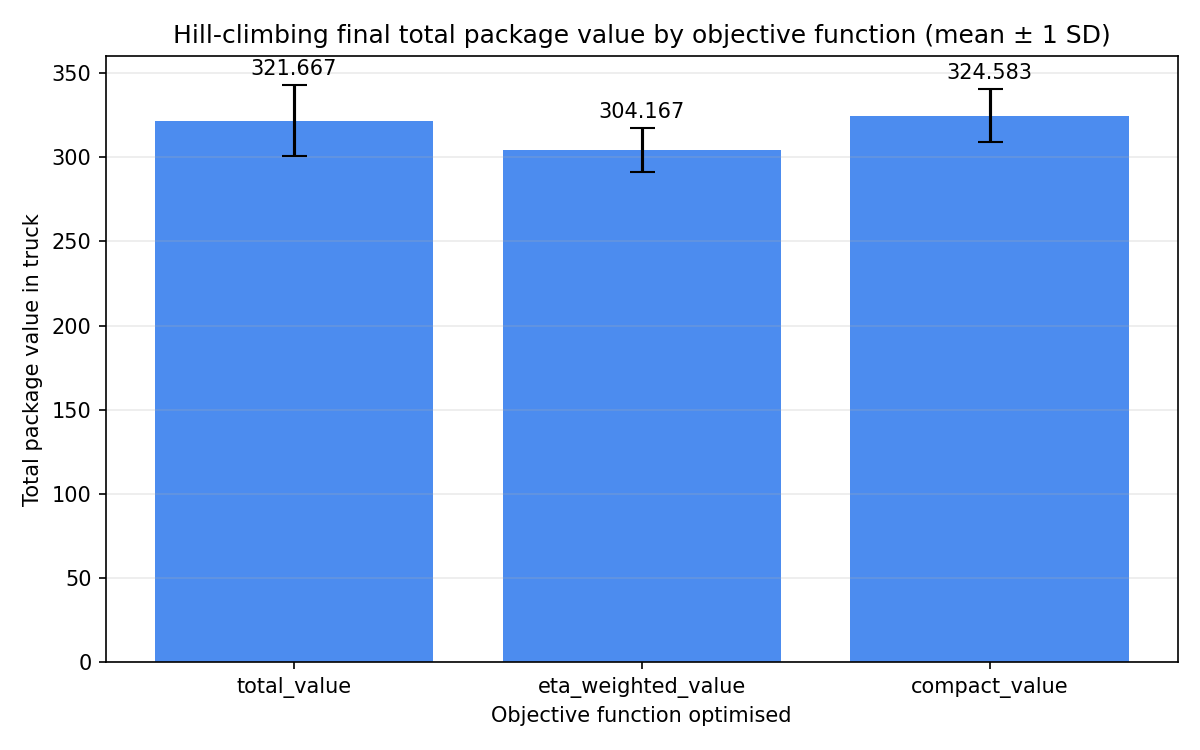
\includegraphics[width=0.85\textwidth]{figures/base/hc-objective-comparison.png}
    \caption{Perbandingan ketiga \textit{objective function} pada \textit{hill climbing}}
\end{figure}

\subsection{Simulated Annealing}

\subsubsection{Fungsi objektif \texttt{total\_value}}
\begin{table}[H]
    \centering
    \begin{tabular}{@{}lrrrr@{}}
        \toprule
        \textit{Objective}            & Rata-rata akhir & Simpangan baku & Nilai total paket & Durasi rata-rata (s)  \\
        \midrule
        \texttt{total\_value}         & 330             & 8,66           & 330               & $0{,}390 \pm 0{,}037$ \\
        \texttt{eta\_weighted\_value} & 116,33          & 0              & 305               & $0{,}375 \pm 0{,}027$ \\
        \texttt{compact\_value}       & 332,04          & 2,79           & 331,67            & $0{,}568 \pm 0{,}043$ \\
        \bottomrule
    \end{tabular}
    \caption{Hasil \textit{simulated annealing} (\texttt{base}, 3 \textit{seed}, 3000 iterasi)}
    \label{tab:sa}
\end{table}

Dengan \texttt{total\_value}, SA mencapai 335 pada \textit{seed} 11 dan 13 serta 320 pada \textit{seed} 12, dengan rata-rata 330. \textit{Seed} 12 berawal dari 285 dan menjadi kasus tersulit bagi hampir semua algoritma. SA keluar dari \textit{local optimum} tersebut dan naik ke 320. Hasil ini lebih tinggi daripada \textit{steepest} dan \textit{sideways} yang berhenti pada 285, serta \textit{stochastic} yang mencapai 290. Namun, SA belum mencapai 335. Riwayat nilai saat ini menunjukkan bahwa SA menerima solusi jauh lebih buruk saat suhu tinggi. Nilai minimum yang dikunjungi adalah 245 pada \textit{seed} 12 dan 255 pada \textit{seed} 11. Seiring pendinginan $0{,}995^{3000}\approx 3\times10^{-7}$, pencarian menyempit ke satu cekungan. Hasil akhir menyimpan solusi terbaik yang pernah dikunjungi, bukan solusi saat pencarian berhenti. Jumlah kejadian \textit{stuck}, saat nilai terbaik tidak berubah selama 100 iterasi berturut-turut, rata-rata 2 per \textit{run}. Nilainya 2, 3, dan 1 untuk \textit{seed} 11, 12, dan 13.

Biaya utama SA adalah waktu pencarian. Algoritma selalu menjalankan 3000 iterasi tanpa berhenti dini, dengan durasi sekitar 0,4 detik per \textit{run}. Durasi ini sekitar 2,5 kali durasi \textit{random restart} dan 74 kali durasi \textit{steepest}.

\begin{figure}[H]
    \centering
    \begin{subfigure}[t]{0.49\textwidth}
        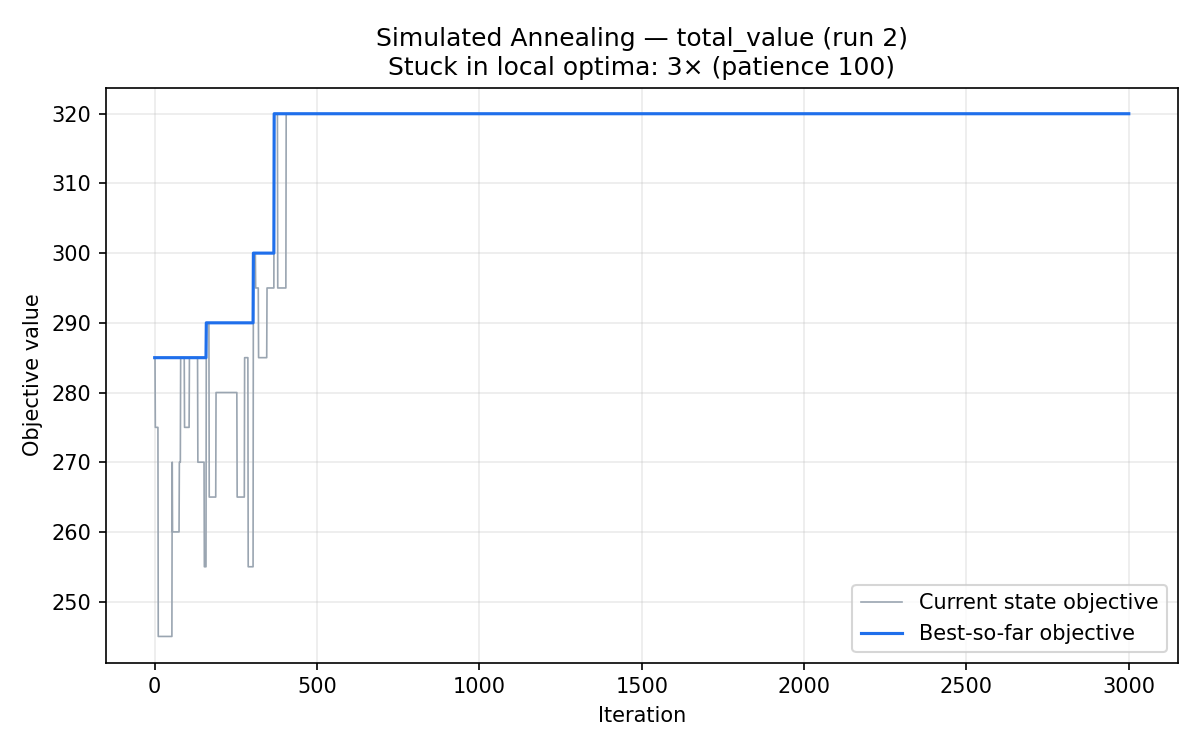
\includegraphics[width=\textwidth]{figures/base/sa-history-total_value-seed12.png}
        \caption{Nilai \textit{objective} (\textit{seed} 12)}
    \end{subfigure}
    \hfill
    \begin{subfigure}[t]{0.49\textwidth}
        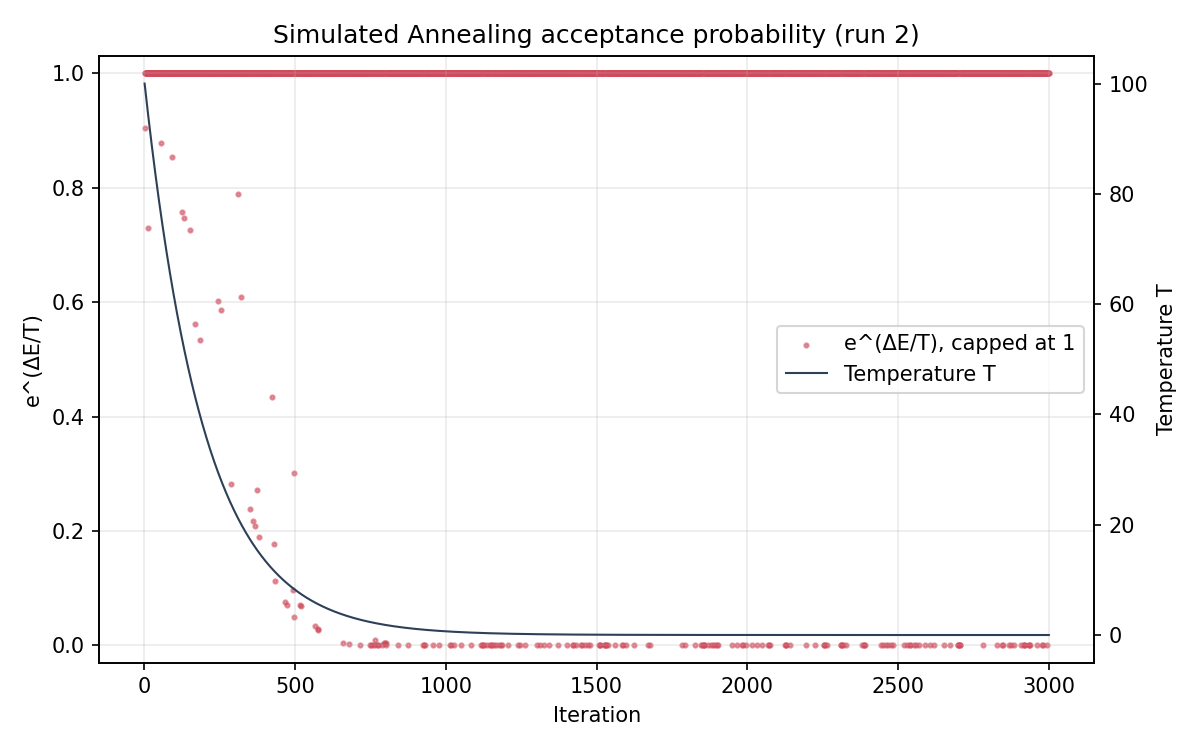
\includegraphics[width=\textwidth]{figures/base/sa-acceptance-total_value-seed12.png}
        \caption{$e^{\Delta E/T}$ terhadap iterasi}
    \end{subfigure}
    \caption{\textit{Simulated annealing} dengan \texttt{total\_value} pada \textit{seed} 12}
\end{figure}

\subsubsection{Fungsi objektif \texttt{eta\_weighted\_value}}
Ketiga \textit{seed} menghasilkan 116,33 dengan simpangan baku 0, sama dengan nilai terbaik yang ditemukan \textit{hill climbing}. Himpunan paket berbeda dari hasil \texttt{total\_value}. Nilai total paketnya 305, bukan 335, tetapi skor ETA mencapai 116,33 dibandingkan 93,45 ketika state hasil \texttt{total\_value} dinilai dengan fungsi ETA, atau naik sekitar 24\%. Jumlah kejadian \textit{stuck} rata-rata 4, dua kali lipat hasil \texttt{total\_value}. Salah satu kemungkinan penyebabnya adalah skala objektif yang lebih kecil membuat suhu awal 100 relatif lebih tinggi. Pengaruh suhu belum diuji dengan variasi $T_0$. Durasi 0,375 detik setara dengan \texttt{total\_value}.

\subsubsection{Fungsi objektif \texttt{compact\_value}}
Nilai akhir pada tiga \textit{seed} adalah 330,449, 330,410, dan 335,254. Rata-ratanya 332,04. Kepadatan rata-rata hasil SA naik dari 0,250 pada \texttt{total\_value} menjadi 0,375, sehingga bonus kepadatan mendorong penataan ke tumpukan yang lebih rendah. Nilai total paket pada masing-masing \textit{seed} adalah 330, 330, dan 335, dengan rata-rata 331,67. Sebagai pembanding, \texttt{total\_value} menghasilkan 335, 320, dan 335. Selisih rata-rata 1,67 berbeda arah antar-seed dan dapat berasal dari \textit{noise}. Durasi rata-rata mencapai 0,568 detik, sekitar 46\% lebih lama daripada 0,390 detik pada \texttt{total\_value}. Penyebab perbedaan durasi ini belum diselidiki.

\begin{figure}[H]
    \centering
    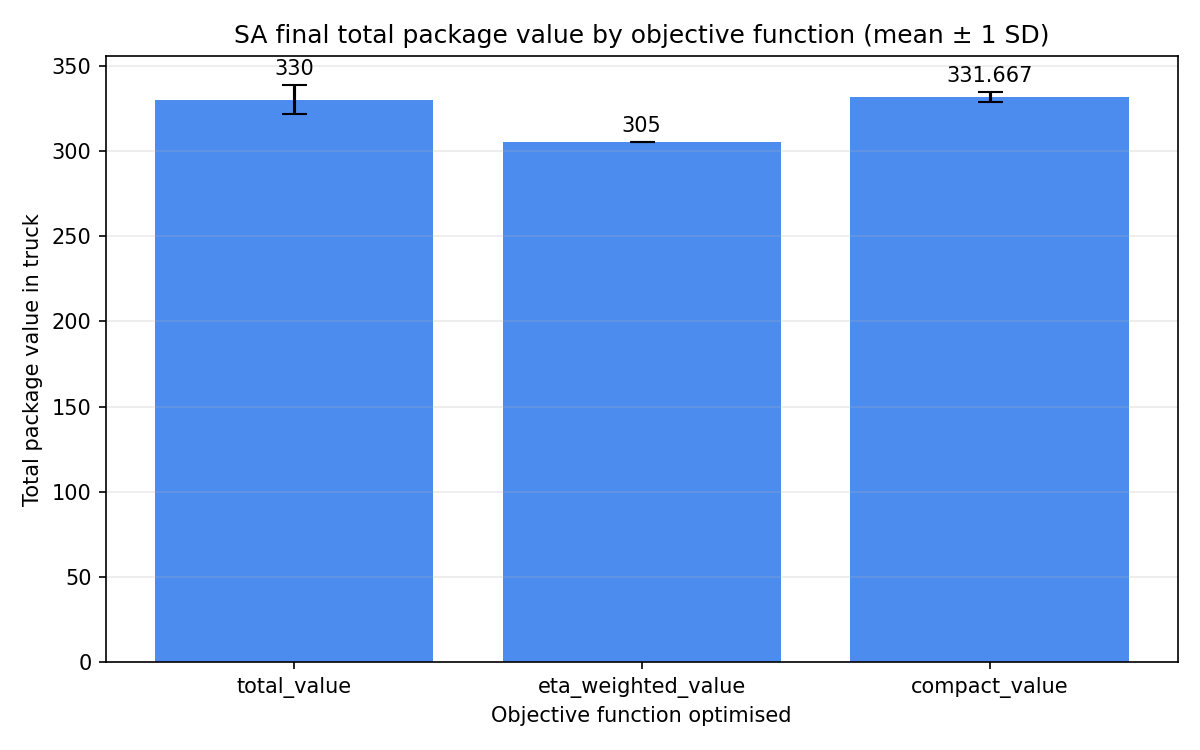
\includegraphics[width=0.85\textwidth]{figures/base/sa-objective-comparison.png}
    \caption{Perbandingan ketiga \textit{objective function} pada \textit{simulated annealing}}
\end{figure}

\subsection{Genetic Algorithm}

\subsubsection{Protokol dan hasil baseline lintas kasus}

Baseline GA dijalankan pada seluruh 11 \textit{fixture} valid dengan \texttt{total\_value}, populasi 20, 40 generasi, \textit{mutation rate} 0,05, dan lima \textit{seed} (11--15), sehingga menghasilkan 55 \textit{run}. Untuk setiap pasangan fixture dan seed, state awal dibuat dari seed turunan yang sama, $s_0=s\oplus\texttt{0x5EED}$. Setiap run melakukan 820 evaluasi objektif, sesuai $(40+1)\times20$. Seluruh state akhir lolos validasi. Pada fixture \texttt{infeasible}, kelima run mengembalikan state kosong yang valid dengan nilai 0 dan tanpa paket termuat.

Tabel~\ref{tab:ga-fixture-baseline} merangkum nilai akhir, variasi antarseed, paket termuat, serta waktu pencarian. Nilai terbaik pada tabel adalah maksimum hasil run yang benar-benar diamati, bukan klaim optimum global. Kasus tanpa pemuatan layak dilaporkan sebagai pemeriksaan validitas, bukan sebagai perbandingan kualitas dengan kasus yang dapat dimuat.

\begin{table}[H]
    \centering
    \small
    \caption{Baseline GA pada seluruh fixture valid. Rata-rata dan simpangan baku sampel dari lima seed}
    \label{tab:ga-fixture-baseline}
    \begin{tabular}{@{}lrrrrr@{}}
        \toprule
        \textit{Fixture}           & Rata-rata nilai $\pm$ SD & Terbaik & Paket termuat & Durasi (s) \\
        \midrule
        \texttt{base}              & 331,00 $\pm$ 2,24        & 335     & 6,0           & 0,681      \\
        \texttt{tight-space}       & 274,00 $\pm$ 10,84       & 290     & 5,0           & 0,543      \\
        \texttt{tight-capacity}    & 174,00 $\pm$ 2,24        & 175     & 3,4           & 0,523      \\
        \texttt{infeasible}        & 0,00 $\pm$ 0,00          & 0       & 0,0           & 0,205      \\
        \texttt{single-package}    & 50,00 $\pm$ 0,00         & 50      & 1,0           & 0,041      \\
        \texttt{equal-fitness}     & 40,00 $\pm$ 0,00         & 40      & 4,0           & 0,339      \\
        \texttt{exact-capacity}    & 100,00 $\pm$ 0,00        & 100     & 3,0           & 0,170      \\
        \texttt{wall-touching}     & 100,00 $\pm$ 0,00        & 100     & 4,0           & 0,233      \\
        \texttt{fragile-support}   & 90,00 $\pm$ 0,00         & 90      & 2,0           & 0,177      \\
        \texttt{rotation-only}     & 70,00 $\pm$ 0,00         & 70      & 1,0           & 0,108      \\
        \texttt{zero-value-weight} & 70,00 $\pm$ 0,00         & 70      & 3,0           & 0,163      \\
        \bottomrule
    \end{tabular}
\end{table}

Perbedaan terhadap kasus dasar terlihat pada ruang truk yang dipersempit. Rata-rata \texttt{tight-space} turun dari 331 pada \texttt{base} menjadi 274, dan simpangan bakunya 10,84 merupakan yang terbesar di antara 11 fixture. Nilai terbaik yang ditemukan pada lima seed adalah 290. Sebaliknya, nilai pada \texttt{tight-capacity} mendekati batas nilai berbasis kapasitas 175, tetapi tidak semua seed mencapainya. Fixture batas berukuran kecil mencapai nilai yang sama pada kelima seed. Konsistensi tersebut menunjukkan bahwa kasus-kasus sederhana ini terjangkau oleh konfigurasi GA, bukan bahwa algoritma selalu menemukan optimum pada instance lain.

\begin{figure}[H]
    \centering
    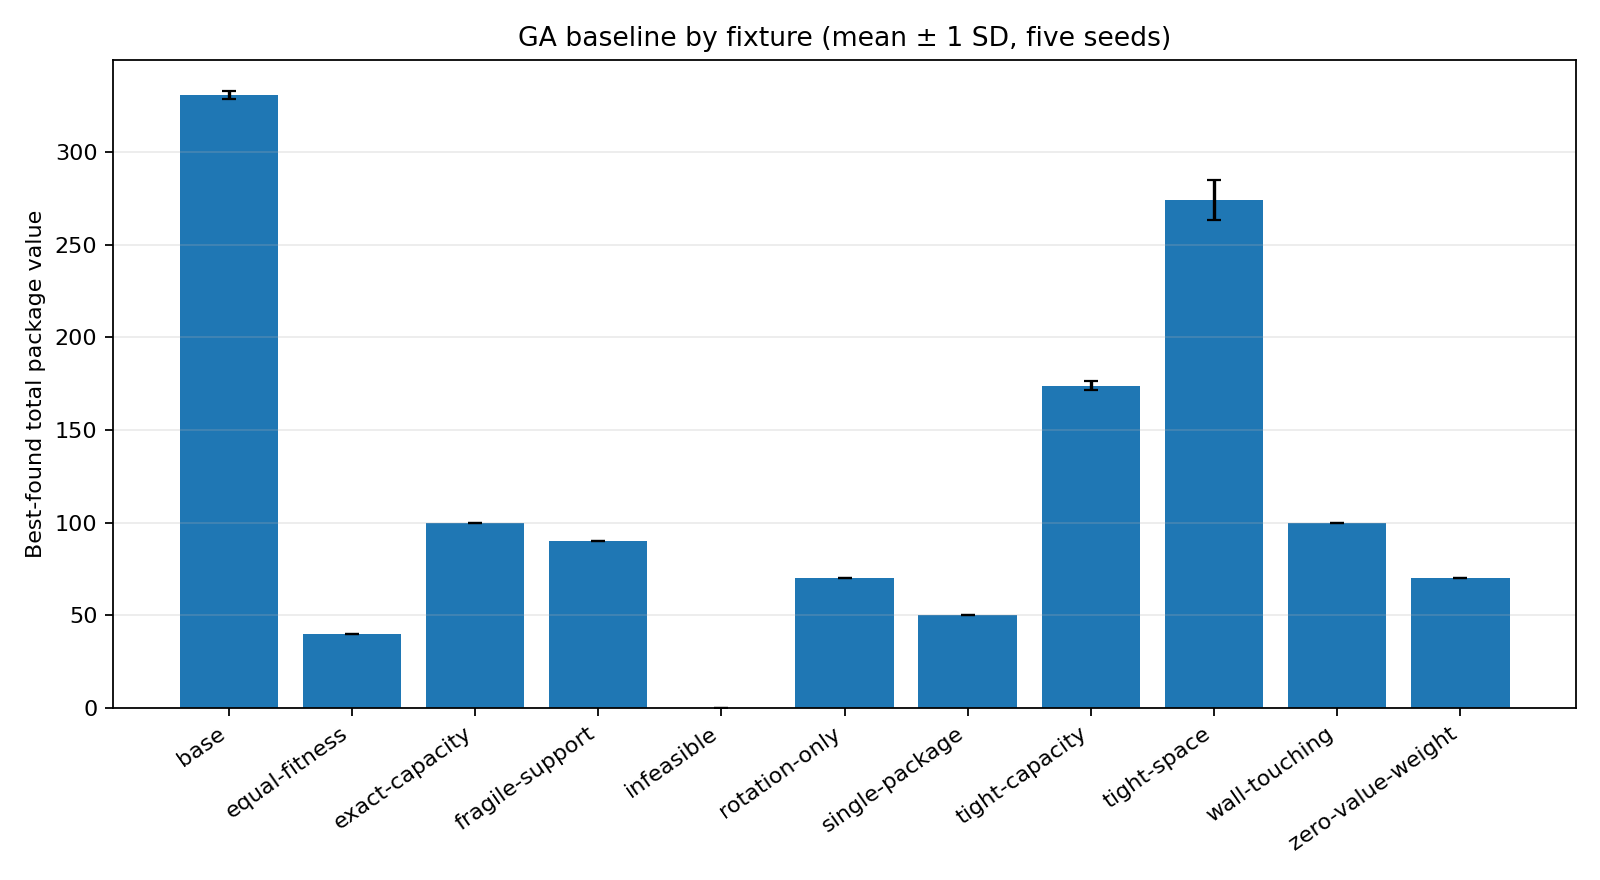
\includegraphics[width=0.92\textwidth]{figures/ga-analysis/fixture-summary.png}
    \caption{Rata-rata nilai terbaik yang ditemukan pada tiap fixture. Batang galat menunjukkan satu simpangan baku sampel}
    \label{fig:ga-fixture-summary}
\end{figure}

\subsubsection{Contoh keluaran dan visualisasi state}

Tabel~\ref{tab:ga-representative} memperlihatkan hasil konkret dari run dengan seed 11, satu run representatif yang dipilih konsisten sebelum melihat perbandingan antarparameter. Kolom paket menunjukkan assignment pada state akhir, bukan seluruh kandidat yang diperiksa GA. Pada \texttt{base}, nilai awal sudah 330 sehingga run tersebut tidak meningkat. Pada \texttt{tight-space} dan \texttt{tight-capacity}, pencarian memperbaiki nilai awal. Kasus \texttt{rotation-only} memuat paket \texttt{long} setelah rotasi, sementara kasus \texttt{infeasible} tetap kosong.

\begin{table}[H]
    \centering
    \small
    \caption{Keluaran aktual GA untuk seed 11 pada satu wakil tiap kategori dan kedua fixture kendala ketat}
    \label{tab:ga-representative}
    \begin{tabular}{@{}lrrrl@{}}
        \toprule
        Kasus                   & Nilai awal $\rightarrow$ akhir & Paket & Valid & Paket termuat pada hasil     \\
        \midrule
        \texttt{base}           & 330 $\rightarrow$ 330          & 6/10  & Ya    & P01, P02, P04, P06, P08, P09 \\
        \texttt{tight-space}    & 255 $\rightarrow$ 270          & 4/10  & Ya    & P02, P04, P07, P09           \\
        \texttt{tight-capacity} & 155 $\rightarrow$ 175          & 3/10  & Ya    & P02, P04, P06                \\
        \texttt{infeasible}     & 0 $\rightarrow$ 0              & 0/10  & Ya    & --                           \\
        \texttt{rotation-only}  & 30 $\rightarrow$ 70            & 1/2   & Ya    & \texttt{long}                \\
        \bottomrule
    \end{tabular}
\end{table}

Gambar~\ref{fig:ga-state-examples} memperlihatkan perubahan penempatan sebelum dan sesudah pencarian pada empat kategori. Gambar~\ref{fig:ga-capacity-states} menambahkan visualisasi \texttt{tight-capacity}, sehingga kedua bentuk kendala ketat dapat dibandingkan. Gambar state untuk semua fixture dan seed pertama tersedia di \texttt{output/ga-analysis/figures/}.

\begin{figure}[H]
    \centering
    \begin{subfigure}[t]{0.49\textwidth}
        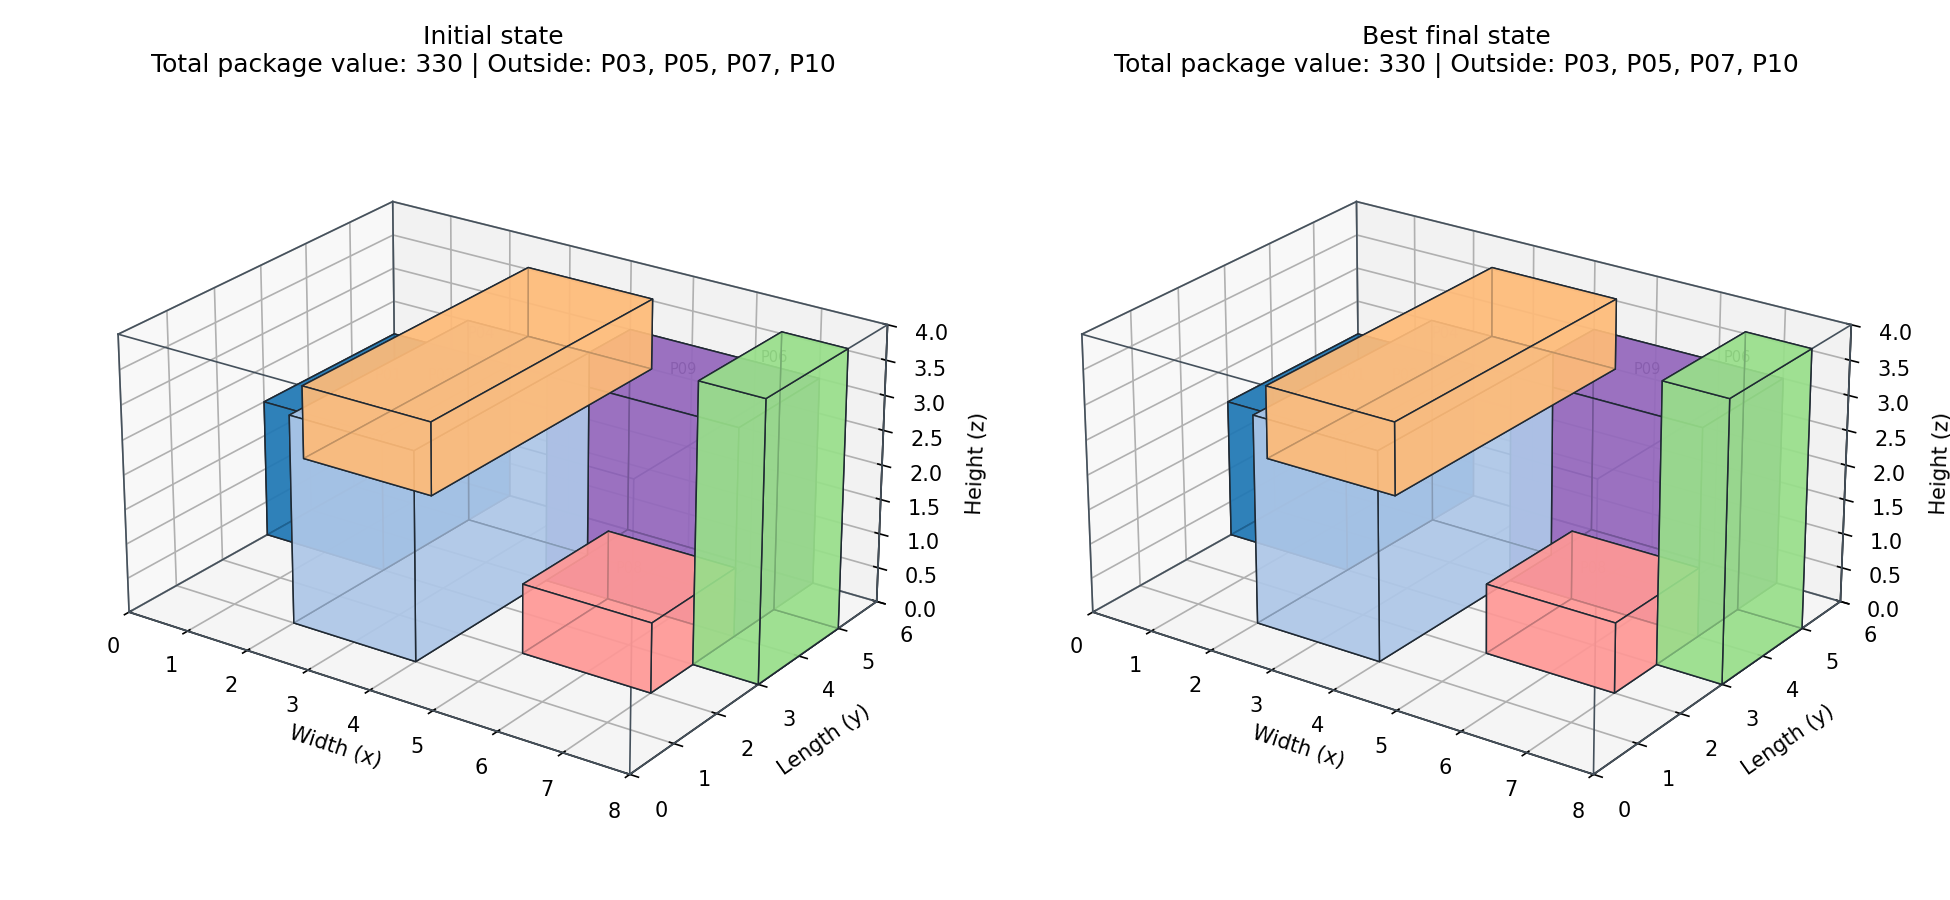
\includegraphics[width=\textwidth]{figures/ga-analysis/base-states.png}
        \caption{Kasus dasar}
    \end{subfigure}
    \hfill
    \begin{subfigure}[t]{0.49\textwidth}
        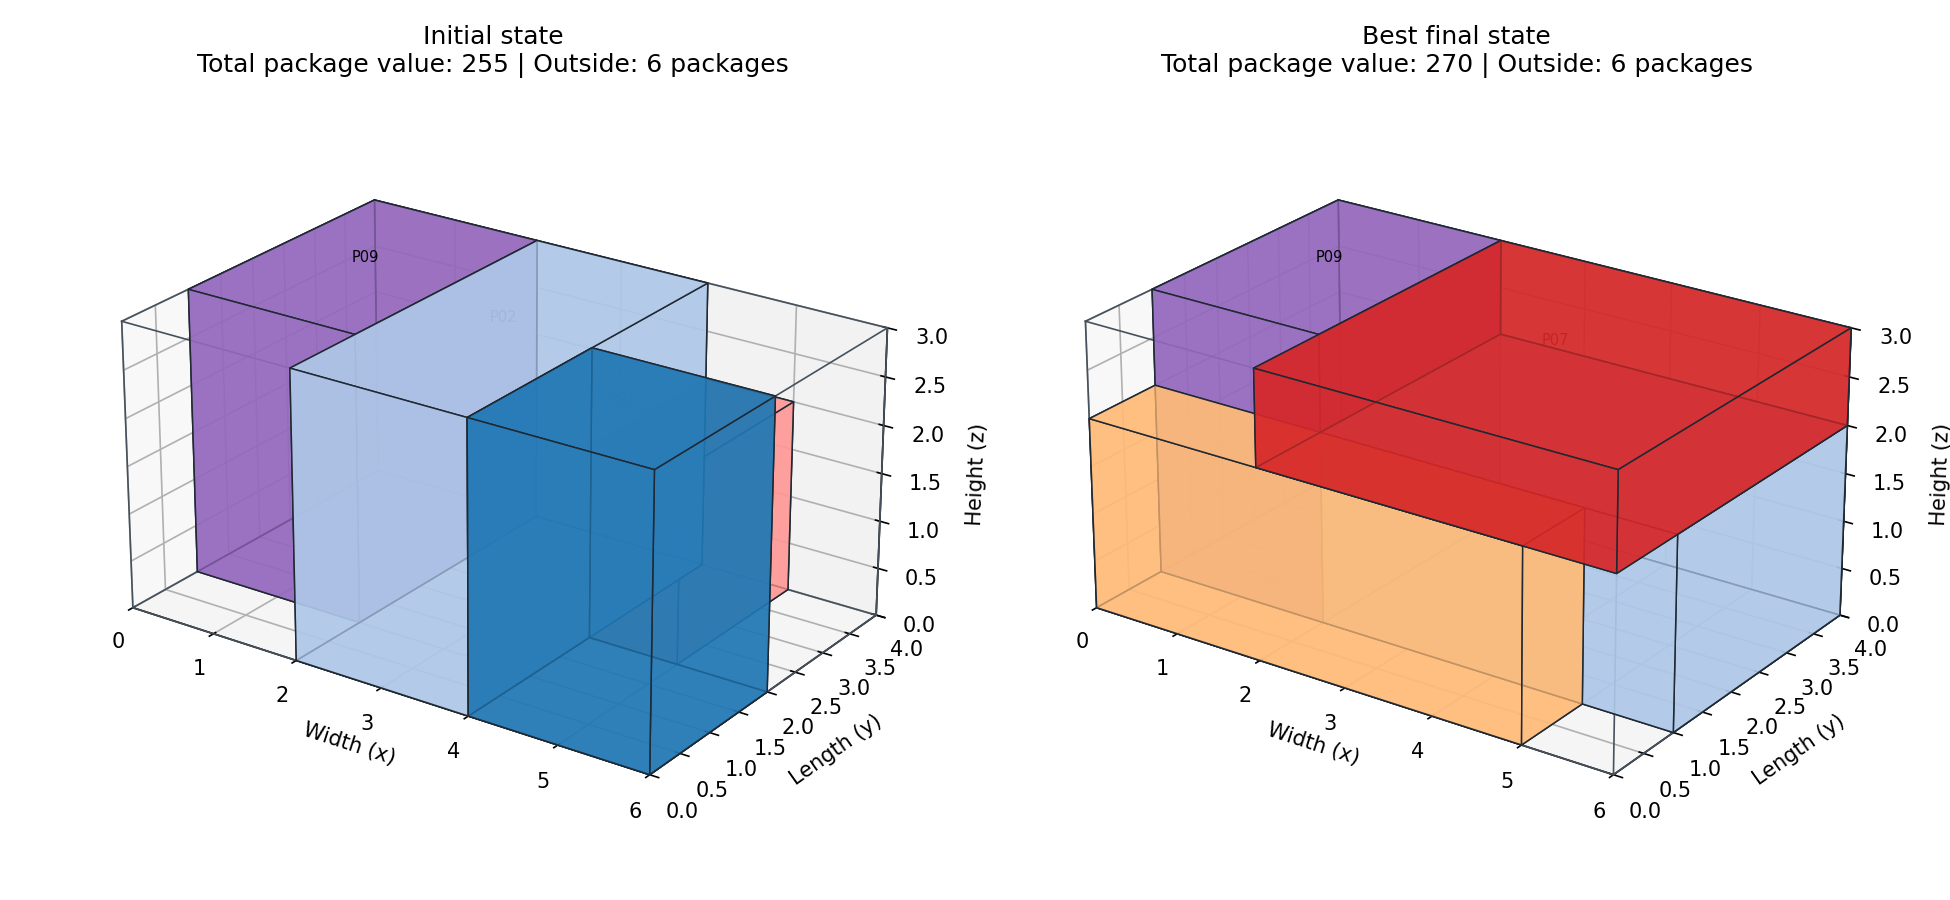
\includegraphics[width=\textwidth]{figures/ga-analysis/tight-space-states.png}
        \caption{Ruang truk ketat}
    \end{subfigure}

    \begin{subfigure}[t]{0.49\textwidth}
        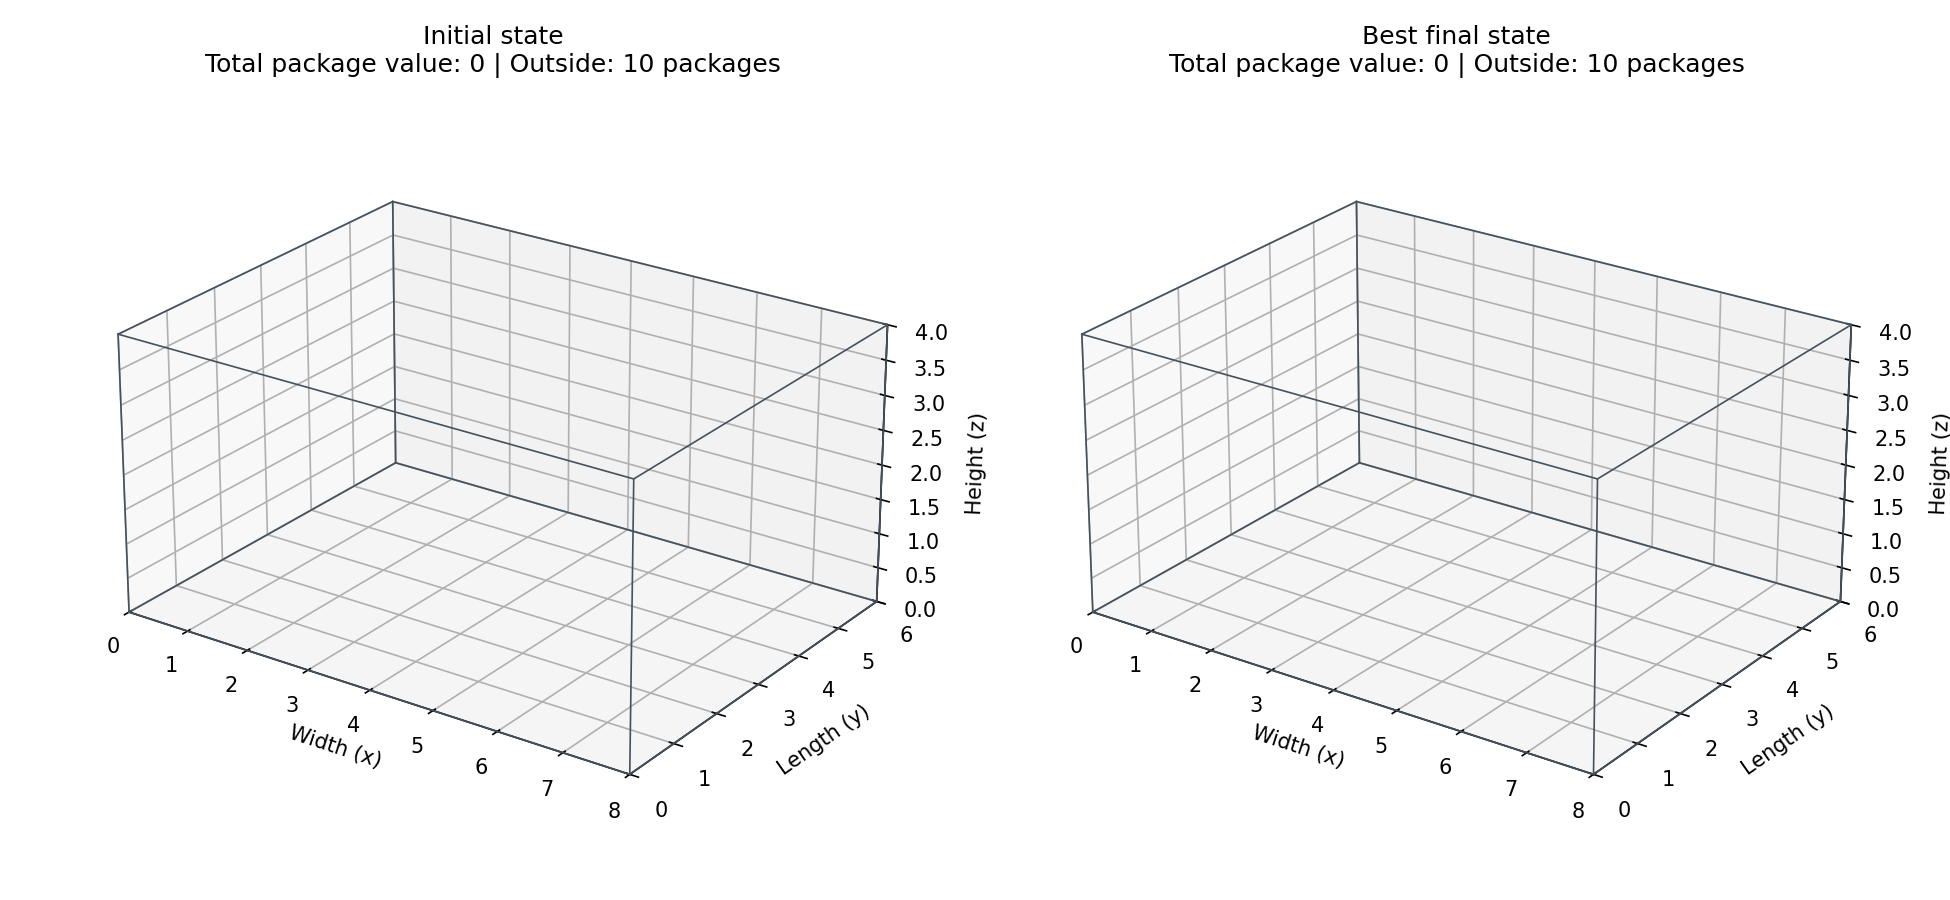
\includegraphics[width=\textwidth]{figures/ga-analysis/infeasible-states.png}
        \caption{Tidak ada pemuatan layak}
    \end{subfigure}
    \hfill
    \begin{subfigure}[t]{0.49\textwidth}
        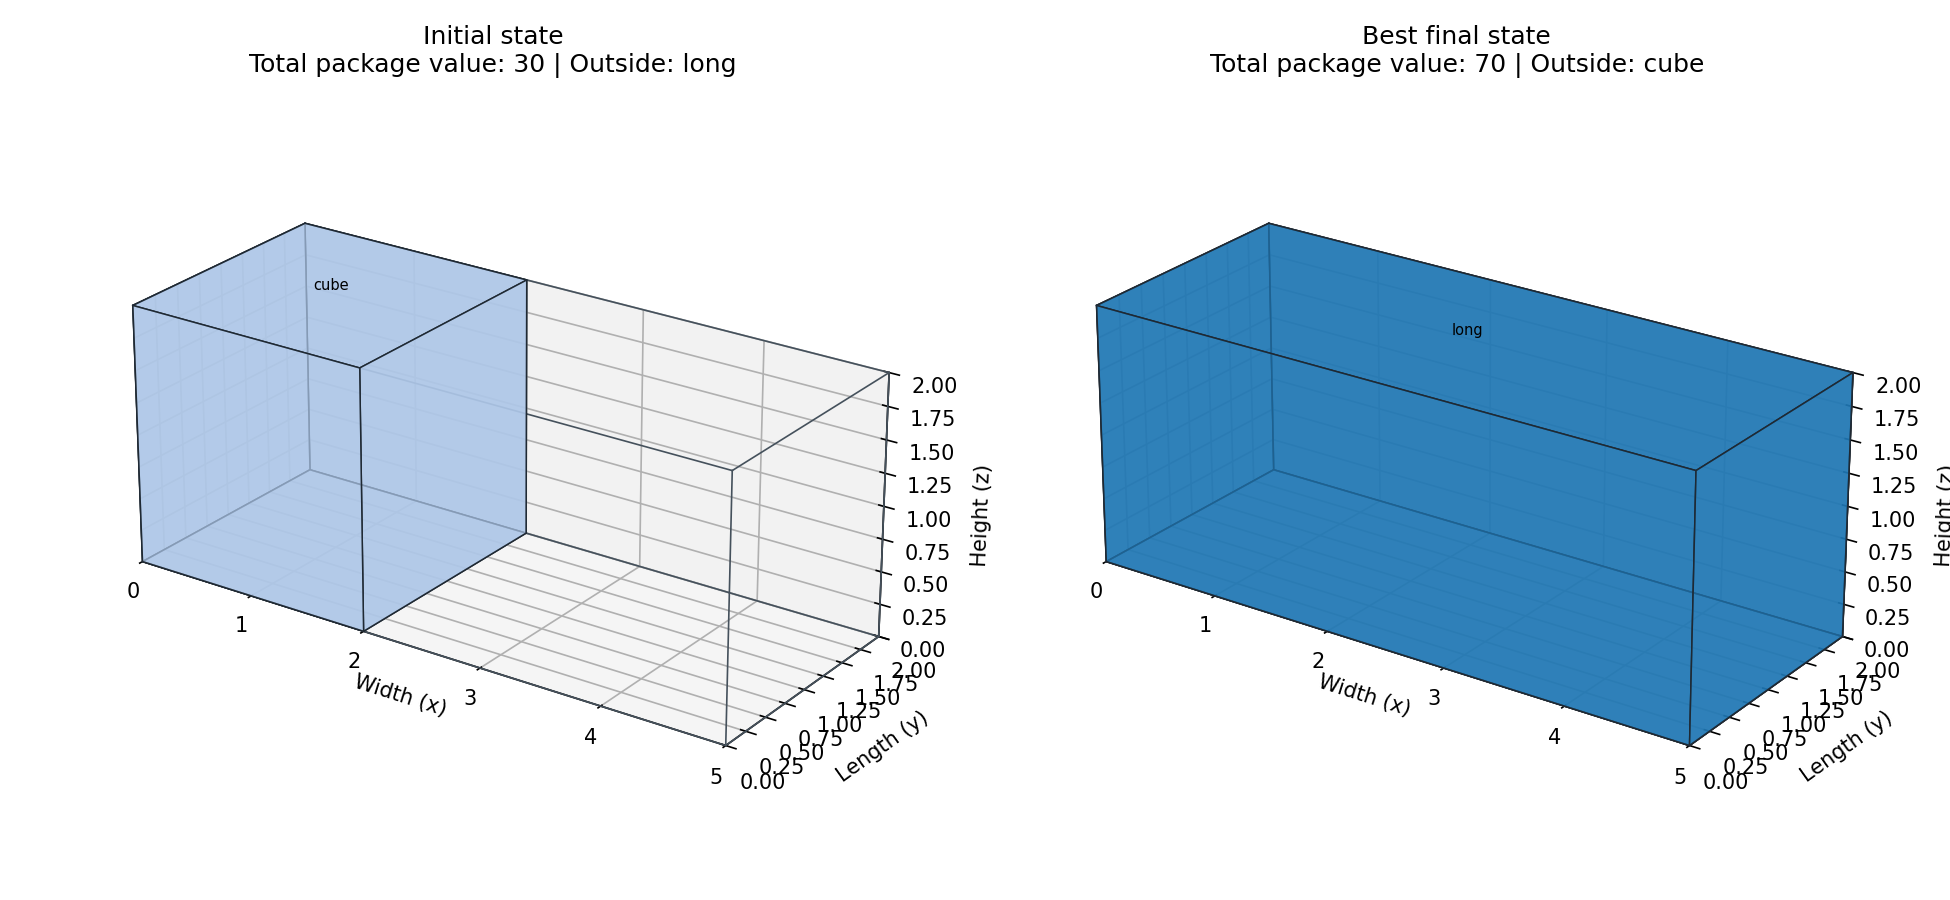
\includegraphics[width=\textwidth]{figures/ga-analysis/rotation-only-states.png}
        \caption{Paket hanya muat setelah rotasi}
    \end{subfigure}
    \caption{State awal dan state terbaik yang dikembalikan GA untuk seed 11}
    \label{fig:ga-state-examples}
\end{figure}

\begin{figure}[H]
    \centering
    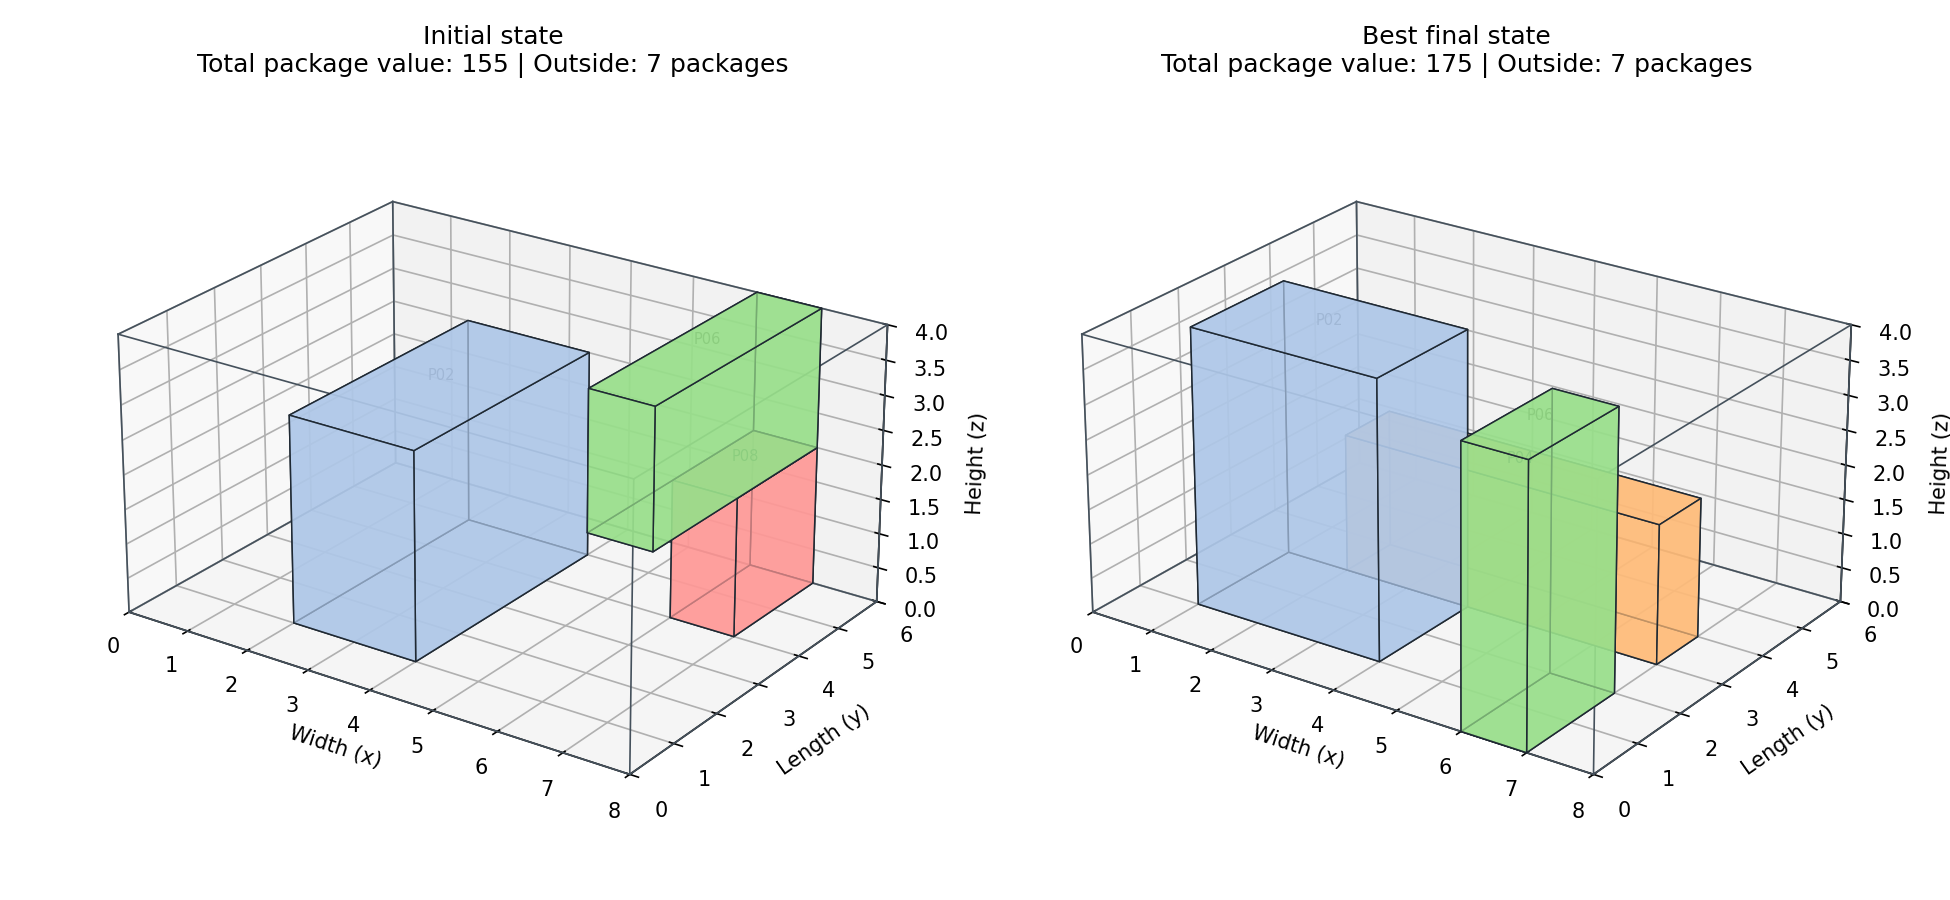
\includegraphics[width=0.92\textwidth]{figures/ga-analysis/tight-capacity-states.png}
    \caption{State awal dan state akhir pada kasus kapasitas truk ketat (seed 11)}
    \label{fig:ga-capacity-states}
\end{figure}

\subsubsection{Pengaruh parameter GA}

Pengaruh ukuran populasi, jumlah generasi, dan laju mutasi diuji secara terpisah pada \texttt{base}. Setiap nilai parameter dijalankan dengan lima seed yang sama dan derivasi state awal yang sama. Parameter lain dipertahankan pada baseline. Tabel~\ref{tab:ga-parameter-sweeps} melaporkan rata-rata nilai terbaik yang ditemukan, simpangan baku sampel, maksimum hasil run, durasi, dan jumlah evaluasi.

\begin{table}[H]
    \centering
    \small
    \caption{Sweep satu faktor GA pada fixture \texttt{base} (lima seed per nilai parameter)}
    \label{tab:ga-parameter-sweeps}
    \begin{tabular}{@{}llrrrr@{}}
        \toprule
        Parameter              & Nilai & Rata-rata $\pm$ SD & Terbaik & Durasi (s) & Evaluasi \\
        \midrule
        Generasi               & 20    & 330,00 $\pm$ 3,54  & 335     & 0,519      & 420      \\
                               & 40    & 331,00 $\pm$ 2,24  & 335     & 0,665      & 820      \\
                               & 80    & 331,00 $\pm$ 2,24  & 335     & 0,935      & 1.620    \\
        \midrule
        Populasi               & 10    & 327,00 $\pm$ 6,71  & 335     & 0,295      & 410      \\
                               & 20    & 331,00 $\pm$ 2,24  & 335     & 0,672      & 820      \\
                               & 40    & 333,00 $\pm$ 2,74  & 335     & 1,553      & 1.640    \\
        \midrule
        \textit{Mutation rate} & 0,00  & 330,00 $\pm$ 0,00  & 330     & 0,623      & 820      \\
                               & 0,05  & 331,00 $\pm$ 2,24  & 335     & 0,659      & 820      \\
                               & 0,20  & 328,00 $\pm$ 4,47  & 330     & 0,809      & 820      \\
        \bottomrule
    \end{tabular}
\end{table}

Ukuran populasi memberi tren kualitas yang paling jelas pada rentang yang diuji. Rata-rata naik dari 327 menjadi 333 saat populasi bertambah dari 10 ke 40, sementara durasi rata-rata meningkat sekitar lima kali (0,295 menjadi 1,553 detik). Namun, nilai terbaik yang pernah ditemukan tetap 335 pada ketiga ukuran populasi, sehingga keuntungan yang terlihat adalah konsistensi rata-rata, bukan batas solusi baru. Karena hanya lima seed yang diuji, tren ini bersifat deskriptif dan tidak membuktikan perbedaan statistik.

Menambah generasi dari 20 menjadi 40 menaikkan rata-rata hanya satu poin (330 ke 331), sedangkan dari 40 ke 80 tidak menambah rata-rata maupun nilai terbaik. Durasi naik dari 0,665 menjadi 0,935 detik. Ini menunjukkan stagnasi hasil pada seed dan rentang generasi ini, bukan bahwa tambahan generasi tidak pernah berguna. Jumlah evaluasi bertambah proporsional dengan ukuran populasi dan banyak generasi karena setiap generasi mengevaluasi seluruh populasi.

Laju mutasi 0,05 memberi rata-rata tertinggi (331) dan satu run mencapai 335. Tanpa mutasi seluruh lima run berakhir pada 330. Laju 0,20 menurunkan rata-rata menjadi 328 dan menghasilkan sebaran lebih lebar (SD 4,47). Pada instance ini, hasil konsisten dengan mutasi moderat membantu mempertahankan variasi yang berguna, sedangkan laju lebih tinggi dapat mengganggu kombinasi yang baik. Lima seed belum cukup untuk menyimpulkan hubungan umum.

Gambar~\ref{fig:ga-parameter-sweeps} memperlihatkan hubungan kualitas dan biaya untuk ketiga sweep. Riwayat pencarian per run disimpan terpisah pada berkas JSON. Grafik di sini menekankan nilai akhir dan durasi agar dampak parameter mudah dibandingkan.

\begin{figure}[H]
    \centering
    \begin{subfigure}[t]{0.49\textwidth}
        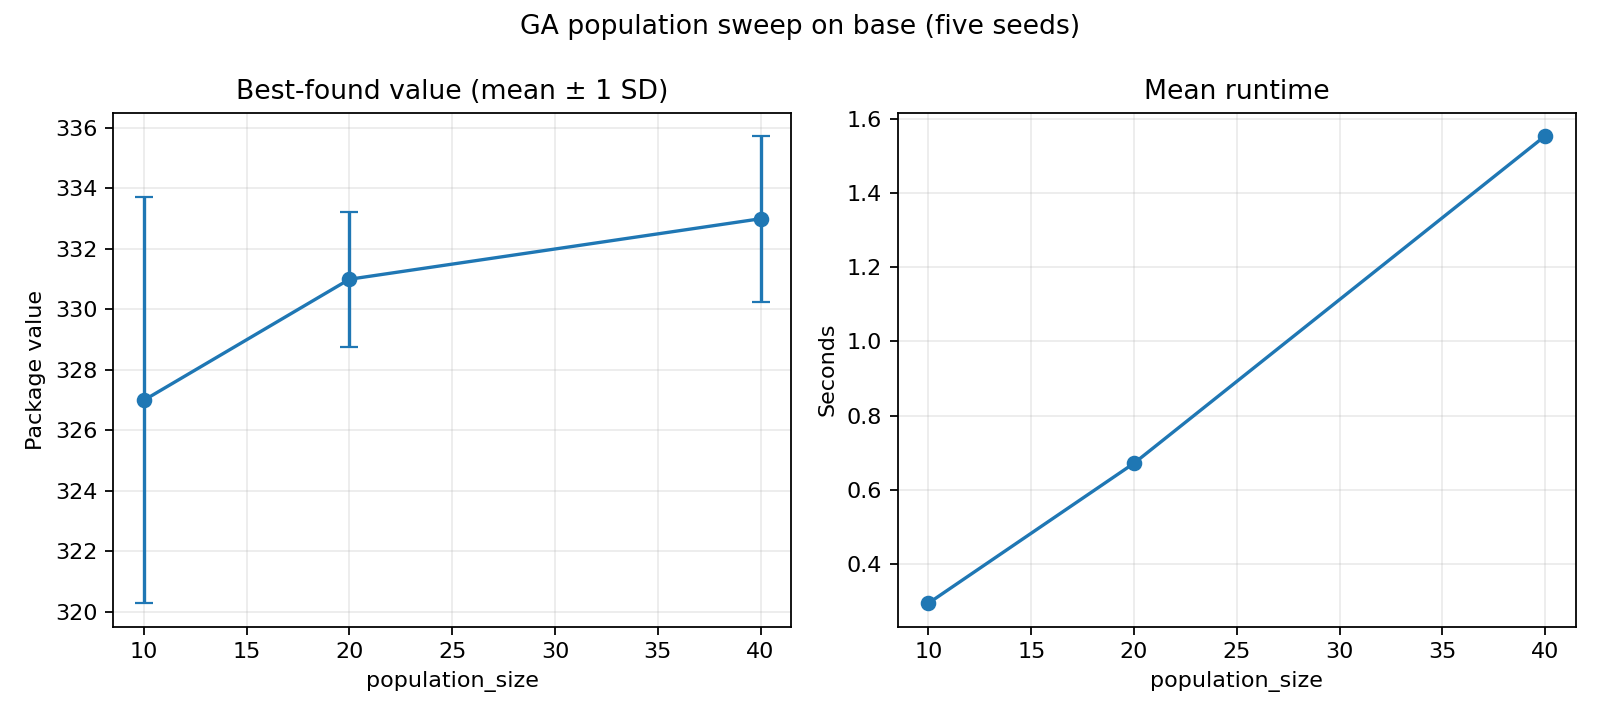
\includegraphics[width=\textwidth]{figures/ga-analysis/population-sweep.png}
        \caption{Ukuran populasi}
    \end{subfigure}
    \hfill
    \begin{subfigure}[t]{0.49\textwidth}
        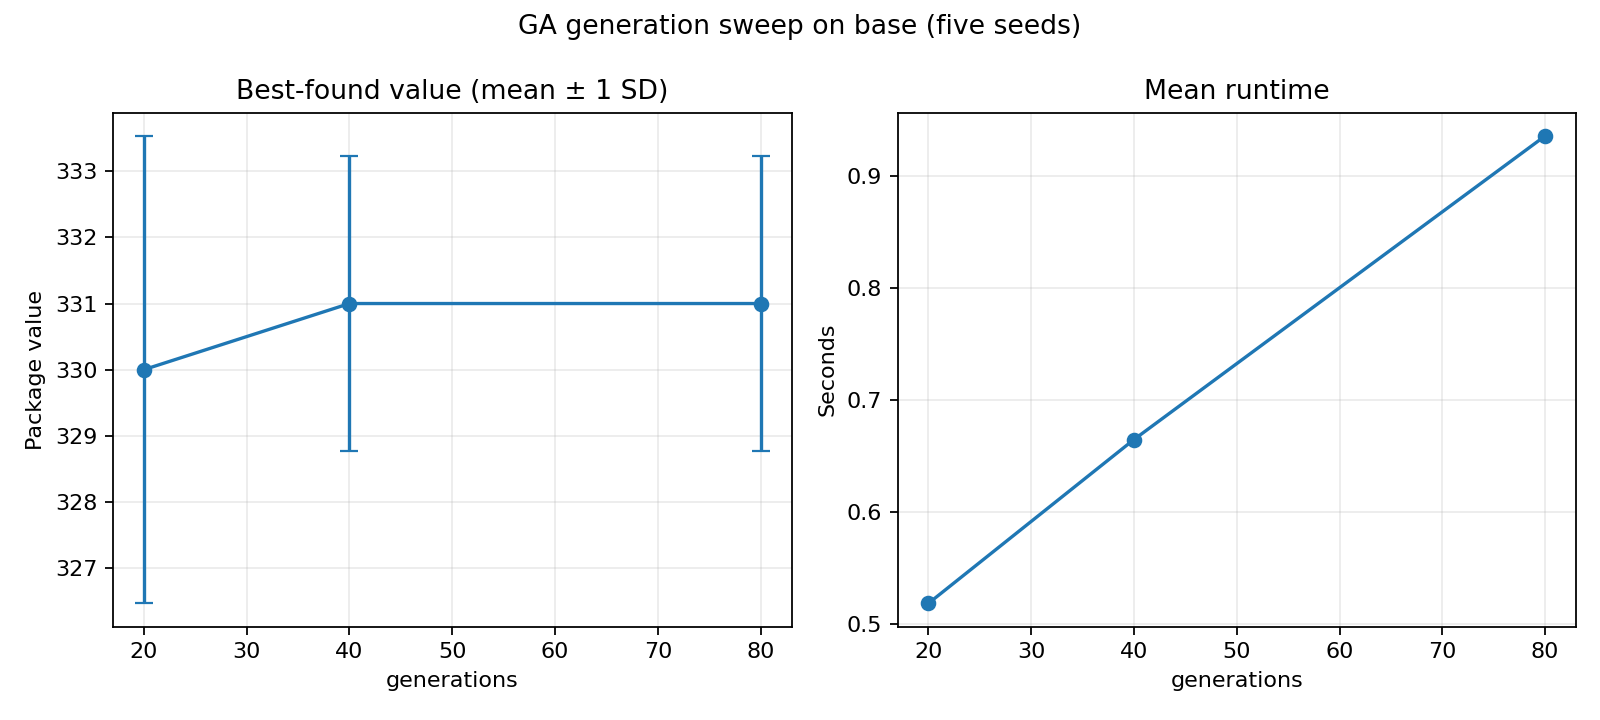
\includegraphics[width=\textwidth]{figures/ga-analysis/generation-sweep.png}
        \caption{Jumlah generasi}
    \end{subfigure}

    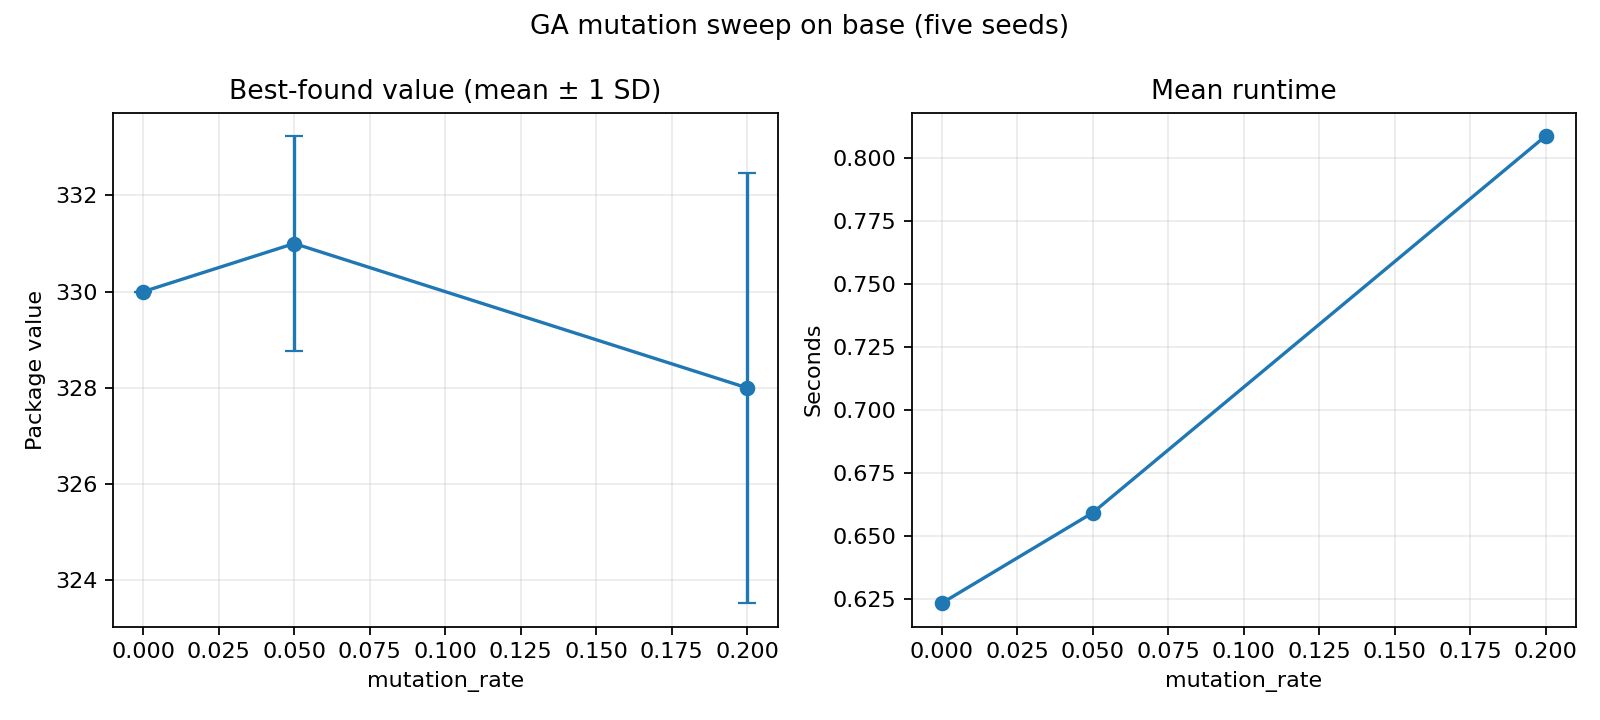
\includegraphics[width=0.78\textwidth]{figures/ga-analysis/mutation-sweep.png}
    \caption{Pengaruh parameter terhadap nilai terbaik dan durasi rata-rata. Batang galat menunjukkan $\pm1$ SD}
    \label{fig:ga-parameter-sweeps}
\end{figure}

Eksperimen ini menggunakan satu fixture untuk sweep parameter dan lima seed, sehingga hasilnya belum menunjukkan konfigurasi terbaik untuk semua kategori. Waktu yang dilaporkan adalah durasi algoritma pada lingkungan lokal yang sama, tetapi dapat berubah akibat beban mesin. Seluruh 100 keluaran per-run, parameter, riwayat objective, dan state awal/akhir disimpan di \texttt{output/ga-analysis/}. Eksperimen dapat direproduksi dengan menjalankan \texttt{python -m src.experiments.ga.results\_analysis} dari root repositori.

\section{Analisis Keseluruhan}

\subsection{Perbandingan Antar-Algoritma pada Seluruh Kategori}

Seluruh 330 \textit{run} \textit{benchmark} menghasilkan \textit{state} akhir yang dinyatakan valid oleh validator. Proporsi valid mencapai 100\%. Ketiga puluh \textit{run} pada \texttt{infeasible} berakhir dengan state kosong yang valid, tanpa paket termuat, dan bernilai 0. Perbandingan kualitas hanya mencakup \textit{instance} yang dapat dimuat. Tabel~\ref{tab:bench-main} merangkum kasus dasar dan kendala ketat. Tabel~\ref{tab:bench-boundary} merangkum kasus batas.

\begin{table}[H]
    \centering
    \small
    \begin{tabular}{@{}lrrrrrrr@{}}
        \toprule
        \textit{Instance}       & Terbaik & \textit{Steepest} & \textit{Sideways} & \textit{Stochastic} & \textit{Restart} & SA          & GA           \\
        \midrule
        \texttt{base}           & 335     & 303,0 (27,5)      & 317,0 (20,5)      & 305,0 (26,2)        & 331,0 (6,5)      & 329,0 (8,2) & 331,0 (2,2)  \\
        \texttt{tight-space}    & 300     & 242,0 (26,8)      & 255,0 (35,0)      & 246,0 (34,4)        & 280,0 (16,2)     & 282,0 (8,4) & 274,0 (10,8) \\
        \texttt{tight-capacity} & 175     & 158,0 (11,5)      & 166,0 (2,2)       & 162,0 (5,7)         & 175,0 (0)        & 173,0 (2,7) & 174,0 (2,2)  \\
        \bottomrule
    \end{tabular}
    \caption{Rata-rata (simpangan baku) nilai akhir \texttt{total\_value}, lima \textit{seed}}
    \label{tab:bench-main}
\end{table}

Frekuensi mencapai nilai terbaik (dari lima \textit{seed}) pada \texttt{base} adalah 1, 2, 1, 3, 3, dan 1 untuk \textit{steepest}, \textit{sideways}, \textit{stochastic}, \textit{random restart}, SA, dan GA. Pada \texttt{tight-space} adalah 0, 1, 1, 1, 0, dan 0. Dan pada \texttt{tight-capacity} adalah 0, 0, 0, 5, 3, dan 4.

\begin{table}[H]
    \centering
    \small
    \begin{tabular}{@{}lrrrrrrr@{}}
        \toprule
        \textit{Instance}          & Terbaik & \textit{Steepest} & \textit{Sideways} & \textit{Stochastic} & \textit{Restart} & SA  & GA  \\
        \midrule
        \texttt{single-package}    & 50      & 50                & 50                & 50                  & 50               & 50  & 50  \\
        \texttt{equal-fitness}     & 40      & 40                & 40                & 40                  & 40               & 40  & 40  \\
        \texttt{exact-capacity}    & 100     & 99                & 100               & 100                 & 100              & 100 & 100 \\
        \texttt{wall-touching}     & 100     & 74                & 98                & 74                  & 100              & 100 & 100 \\
        \texttt{zero-value-weight} & 70      & 58                & 70                & 58                  & 70               & 70  & 70  \\
        \texttt{fragile-support}   & 90      & 78                & 78                & 78                  & 90               & 78  & 90  \\
        \texttt{rotation-only}     & 70      & 46                & 46                & 46                  & 70               & 46  & 70  \\
        \bottomrule
    \end{tabular}
    \caption{Rata-rata nilai akhir \texttt{total\_value} pada kasus batas, lima \textit{seed}}
    \label{tab:bench-boundary}
\end{table}

\begin{table}[H]
    \centering
    \small
    \begin{tabular}{@{}lrrrrrr@{}}
        \toprule
                                      & \textit{Steepest} & \textit{Sideways} & \textit{Stochastic} & \textit{Restart} & SA     & GA     \\
        \midrule
        Evaluasi objektif (rata-rata) & 43                & 3085              & 1001                & 383              & 3001   & 820    \\
        Durasi (s)                    & 0,0056            & 0,4699            & 0,1432              & 0,1543           & 0,5654 & 0,4746 \\
        Durasi per evaluasi (ms)      & 0,13              & 0,15              & 0,14                & 0,40             & 0,19   & 0,58   \\
        \bottomrule
    \end{tabular}
    \caption{Biaya pencarian pada \texttt{base} (lima \textit{seed})}
    \label{tab:bench-cost}
\end{table}

\begin{figure}[H]
    \centering
    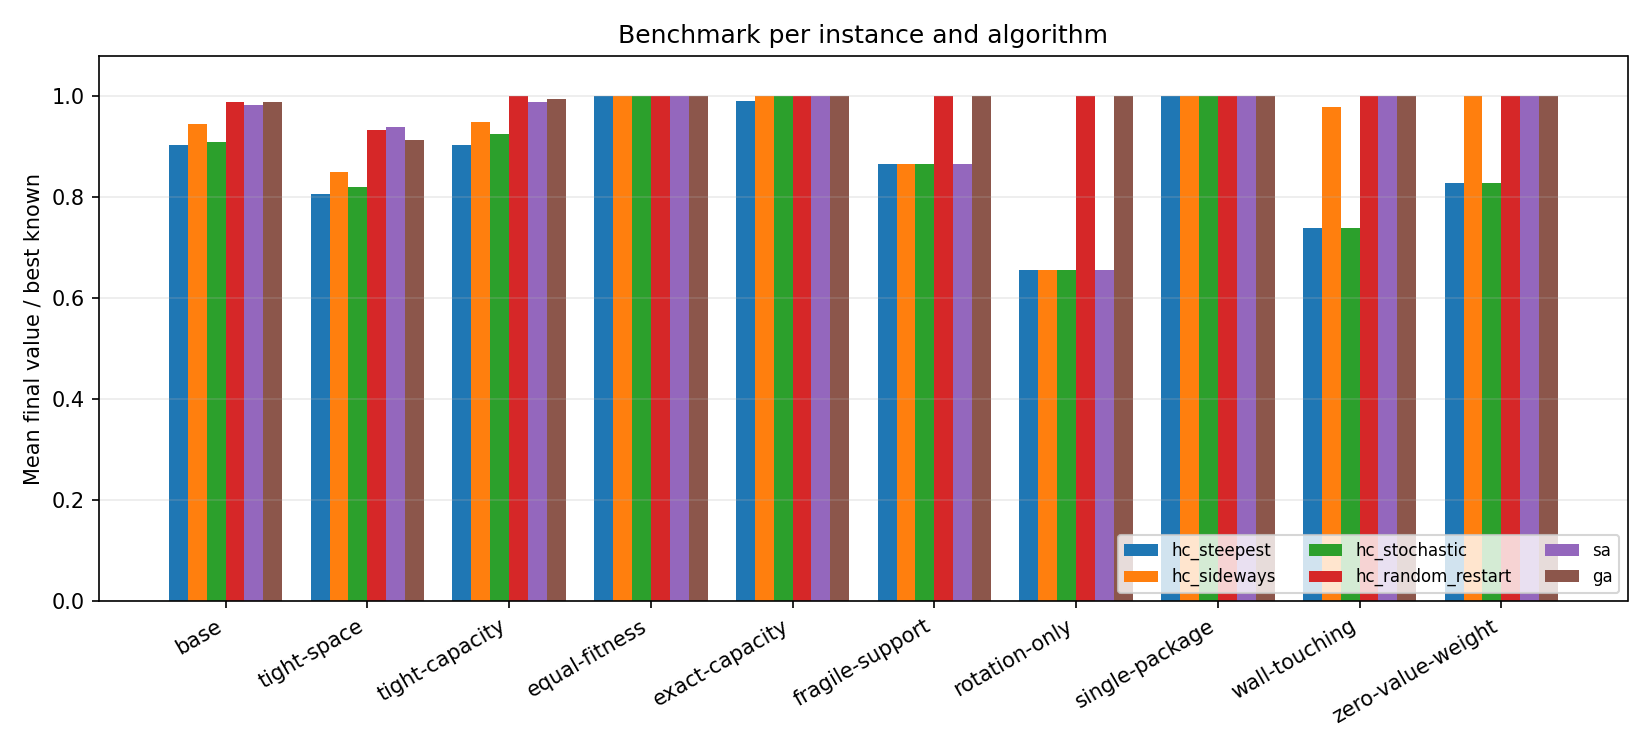
\includegraphics[width=\textwidth]{figures/base/benchmark-summary.png}
    \caption{Rata-rata nilai akhir terhadap nilai terbaik pada tiap \textit{instance} dan algoritma}
\end{figure}

Beberapa pola konsisten muncul.

\begin{enumerate}
    \item \textbf{Kualitas.} Pada \texttt{base} dan \texttt{tight-capacity}, rata-rata \textit{random restart}, SA, dan GA berbeda sekitar 1\%. Rata-rata \textit{steepest}, \textit{sideways}, dan \textit{stochastic} tertinggal 5--10\%. Pada \texttt{tight-space}, SA memperoleh 282, sedikit di atas \textit{random restart} dengan 280 dan GA dengan 274. Tidak ada metode yang mencapai rata-rata 300. \textit{Steepest}, SA, dan GA juga tidak pernah mencapai 300 dalam lima \textit{seed}. Kesulitan pada ruang kecil tampaknya berasal dari penataan geometris, bukan pemilihan paket, karena batas \textit{knapsack} sebesar 335 jauh di atas 300. Selisih rata-rata antara ketiga metode tersebut lebih kecil daripada simpangan bakunya. Lima \textit{seed} belum cukup untuk menyatakan perbedaan yang nyata.
    \item \textbf{Konsistensi.} GA memiliki simpangan baku terkecil pada \texttt{base} (2,2) dan SA pada \texttt{tight-space} (8,4). Tiga varian pertama \textit{hill climbing} memiliki simpangan baku terbesar pada \texttt{base} dan \texttt{tight-space} (20--35). \textit{Random restart} menurunkan simpangan baku varian dasarnya (27,5 menjadi 6,5 pada \texttt{base}, dan 11,5 menjadi 0 pada \texttt{tight-capacity}). Pada \texttt{tight-capacity}, \textit{random restart} mencapai optimum 175 pada kelima \textit{seed}.
    \item \textbf{Biaya.} \textit{Steepest} paling murah dengan 43 evaluasi dan durasi 0,006 detik. \textit{Random restart} memakai 383 evaluasi, sekitar seperdelapan dari SA yang memakai 3001 dan setengah dari GA yang memakai 820, dengan kualitas yang sebanding. Durasi per evaluasi GA sekitar empat kali durasi \textit{steepest} karena juga mencakup pembentukan populasi, \textit{crossover}, perbaikan, dan validasi. Perbandingan biaya perlu melihat durasi bersama jumlah evaluasi.
    \item \textbf{Ketahanan terhadap \textit{local optimum}.} Pada \texttt{base}, perbedaan hasil muncul dari cara algoritma menangani state awal yang buruk. Varian HC yang hanya menerima gerakan setara atau lebih baik dapat tersangkut. SA dapat keluar dengan menerima gerakan yang memburuk saat suhu tinggi. \textit{Random restart} dan GA dapat memulai pencarian dari state acak lain.
\end{enumerate}

\subsection{Ketahanan pada Kasus Batas dan Masukan Tidak Valid}

\textbf{Tanpa pemuatan layak.} Seluruh 30 \textit{run} pada \texttt{infeasible} mengembalikan \textit{state} valid tanpa paket termuat dan nilai 0, sehingga representasi yang mengizinkan semua paket berada di luar truk bekerja seperti yang dirancang. Karena nilai 0 saja ambigu bila ada paket bernilai nol, jumlah paket termuat dicatat bersamaan (0 pada seluruh \textit{run}).

\textbf{Kasus batas.} Kasus \texttt{single-package} dan \texttt{equal-fitness} tidak membedakan algoritma karena \textit{state} awal acak sudah optimal (50 dan 40). Keduanya hanya menunjukkan bahwa seleksi \textit{roulette-wheel} dengan fitness yang sama dan satu paket tidak menimbulkan galat. Kasus lain membedakan algoritma dengan jelas. 
\begin{itemize}
    \item \texttt{rotation-only}. \textit{Random restart} dan GA mencapai 70 pada kelima \textit{seed}. Empat metode lain hanya mencapai 70 pada dua \textit{seed} yang state awalnya sudah memuat paket panjang. Pada tiga state awal lainnya, rata-ratanya tetap 46. Operator \textit{move} tidak mengeluarkan paket dari truk. Operator \textit{swap} memberi orientasi awal $(0,1,2)$ kepada paket dari luar, sehingga paket $2\times2\times5$ tidak muat. Paket panjang tidak dapat dimasukkan selama paket kubus berada di dalam. Karena itu, dari state tersebut tidak ada jalur menuju state yang lebih baik dengan operator yang tersedia. Ini merupakan batasan operator \textit{neighbor}. \textit{Random restart} dan GA dapat menghindarinya dengan membangkitkan state awal baru.
    \item \texttt{fragile-support}. \textit{Random restart} dan GA mencapai 90 pada seluruh \textit{seed} dengan menempatkan paket rapuh di atas paket yang tidak rapuh. Empat metode lain mendapat nilai 60 pada dua dari lima \textit{seed} dan rata-rata 78. Ketiganya mencapai 90 pada tiga \textit{seed} lainnya.
    \item \texttt{wall-touching}. \textit{Random restart}, SA, dan GA mengisi truk hingga tepat menyentuh dinding dan mendapat nilai 100 pada seluruh \textit{seed}. Nilai rata-rata \textit{sideways} adalah 98, sedangkan \textit{steepest} dan \textit{stochastic} memperoleh 74. Validator menerima penempatan yang menyentuh dinding pada seluruh \textit{run}.
    \item \texttt{exact-capacity}. Seluruh algoritma mencapai 100 (berat tepat sama dengan kapasitas) kecuali satu \textit{run} \textit{steepest} pada 95, sehingga batas ``$\leq$'' pada kapasitas ditangani benar.
    \item \texttt{zero-value-weight}. \textit{Steepest} dan \textit{stochastic} berakhir pada nilai 10 pada satu \textit{seed}, yaitu seed 13. Paket berbobot nol termuat tanpa paket \texttt{regular}. Algoritma lain selalu memperoleh nilai 70. Paket bernilai nol atau berbobot nol tidak menyebabkan galat maupun state tidak valid.
\end{itemize}

\textbf{Masukan tidak valid.} Seluruh delapan \textit{fixture} pada \texttt{invalid/} ditolak oleh \textit{loader} dengan \texttt{ValueError} dan pesan yang menyebut penyebabnya (Tabel~\ref{tab:invalid}). Tidak ada yang lolos ke pencarian.

\begin{table}[H]
    \centering
    \small
    \begin{tabular}{@{}p{5.2cm}p{9.5cm}@{}}
        \toprule
        \textit{Fixture}                       & Pesan galat                                                      \\
        \midrule
        \texttt{package-dimension-nonpositive} & \textit{package dimensions must contain three positive integers} \\
        \texttt{package-dimension-length}      & \textit{packages[0].dimensions must be a list of three integers} \\
        \texttt{package-dimension-noninteger}  & \textit{packages[0].dimensions must be a list of three integers} \\
        \texttt{truck-dimension-nonpositive}   & \textit{truck dimensions must contain three positive integers}   \\
        \texttt{truck-capacity-negative}       & \textit{truck capacity must be a non-negative integer}           \\
        \texttt{duplicate-ids}                 & \textit{package IDs must be unique}                              \\
        \texttt{empty-packages}                & \textit{problem must contain at least one package}               \\
        \texttt{missing-field}                 & \textit{packages[0] is missing 'eta'}                            \\
        \bottomrule
    \end{tabular}
    \caption{Penolakan masukan tidak valid oleh \textit{loader}}
    \label{tab:invalid}
\end{table}

\subsection{Pengaruh Variasi \textit{Objective Function}}

\begin{table}[H]
    \centering
    \small
    \begin{tabular}{@{}llrrrrr@{}}
        \toprule
        \textit{Instance}       & Algoritma              & \multicolumn{3}{c}{Nilai total paket rata-rata} & \multicolumn{2}{c}{Durasi (s)}                                                        \\
        \cmidrule(lr){3-5}\cmidrule(lr){6-7}
                                &                        & \texttt{total}                                  & \texttt{eta}                   & \texttt{compact} & \texttt{total} & \texttt{compact} \\
        \midrule
        \texttt{base}           & \textit{Hill climbing} & 321,67                                          & 304,17                         & 324,58           & 0,198          & 0,176            \\
                                & SA                     & 330                                             & 305                            & 331,67           & 0,390          & 0,568            \\
                                & GA                     & 331,39                                          & 296,94                         & 331,39           & 0,447          & 0,441            \\
        \midrule
        \texttt{tight-capacity} & \textit{Hill climbing} & 165                                             & 153,75                         & 165,83           & 0,080          & 0,084            \\
                                & SA                     & 173,33                                          & 170                            & 171,67           & 0,285          & 0,314            \\
                                & GA                     & 174,17                                          & 166,94                         & 174,17           & 0,397          & 0,316            \\
        \bottomrule
    \end{tabular}
    \caption{Nilai total paket pada \textit{state} akhir menurut \textit{objective} yang dioptimalkan (\texttt{total} = \texttt{total\_value}, \texttt{eta} = \texttt{eta\_weighted\_value}, \texttt{compact} = \texttt{compact\_value}). Durasi untuk \texttt{total\_value} dan \texttt{compact\_value}}
    \label{tab:objective}
\end{table}

Nilai total paket pada Tabel~\ref{tab:objective} dihitung ulang dengan \texttt{total\_value} untuk seluruh \textit{state} akhir, sehingga ketiga \textit{objective} dapat dibandingkan pada satu skala. \texttt{eta\_weighted\_value} jelas mengubah himpunan paket. Pada kedua \textit{instance} dan ketiga algoritma nilai total turun (misalnya GA pada \texttt{base} dari 331,39 menjadi 296,94, dan SA dari 330 menjadi 305), sedangkan skor ETA yang dioptimalkan naik (SA pada \texttt{base} dari 93,45 menjadi 116,33). \texttt{compact\_value} tidak mengorbankan nilai total dan nilai akhirnya sama dengan atau sedikit di atas \texttt{total\_value}. Selisih kecil pada HC dan SA lebih mungkin berasal dari gradien kepadatan yang membantu pencarian melewati dataran (Tabel~\ref{tab:hc-compact}) daripada dari perubahan himpunan paket. Pada GA \texttt{compact\_value} memberi nilai total yang identik dengan \texttt{total\_value} (331,39 dan 174,17).

Efek \texttt{compact\_value} pada penataan terukur pada SA. Kepadatan rata-rata naik dari 0,250 menjadi 0,375 pada \texttt{base} dan dari 0,305 menjadi 0,614 pada \texttt{tight-capacity}. Biaya komputasi ketiga \textit{objective} sebanding pada HC dan GA (selisih durasi rata-rata hingga sekitar 25\% pada kedua \textit{instance}), tetapi SA dengan \texttt{compact\_value} lebih lambat pada \texttt{base} (0,568 dibanding 0,390 detik), perbedaan yang tidak terlihat pada \texttt{tight-capacity} (0,314 dibanding 0,285 detik) dan belum ditelusuri penyebabnya.

\subsection{Keterbatasan}
Seluruh \textit{instance} bersifat sintetis dan kecil (1--10 paket), dan konfigurasi per algoritma hanya diulang tiga kali (lima kali pada \textit{benchmark} dan ablasi). Akibatnya selisih yang kecil, seperti antara \textit{random restart}, SA, dan GA pada \texttt{base}, tidak dapat dibedakan dari \textit{noise}. Parameter tiap algoritma (suhu awal, laju pendinginan, ukuran populasi, \textit{mutation rate}, jumlah tetangga per iterasi) tidak disetel, hanya satu konfigurasi yang dipakai pada \textit{benchmark}, sehingga urutan algoritma berlaku untuk konfigurasi tersebut. Optimum sebenarnya hanya diketahui untuk \texttt{base} dan \texttt{tight-capacity} (lewat batas atas \textit{knapsack}). Untuk \texttt{tight-space} nilai ``terbaik'' hanyalah yang tertinggi yang ditemukan. Hasil pada data paket kelompok yang sesungguhnya, jika ada dan berbeda, perlu ditambahkan pada bagian ini.

\section{Analisis Implementasi Spesifikasi Bonus}

\subsection{\textit{Extra} Objective Function}

Dua fungsi objektif tambahan, \texttt{eta\_weighted\_value} dan \texttt{compact\_value}, diuji dengan algoritma, \textit{seed}, dan \textit{state} awal yang sama seperti \texttt{total\_value} (Tabel~\ref{tab:objective}).

\begin{enumerate}
    \item \textbf{\texttt{eta\_weighted\_value} mengubah pilihan paket saat nilai dan urgensi berbeda.} Pada \texttt{base}, nilai total paket turun dari 321,67 menjadi 304,17 untuk HC, dari 330 menjadi 305 untuk SA, dan dari 331,39 menjadi 296,94 untuk GA. Skor ETA SA naik dari 93,45 menjadi 116,33. Pada \texttt{tight-capacity}, nilai HC turun dari 165 menjadi 153,75, SA dari 173,33 menjadi 170, dan GA dari 174,17 menjadi 166,94. Skor objektif ini lebih kecil, dengan maksimum 116,33 pada \texttt{base} dan 75,83 pada \texttt{tight-capacity}. Parameter yang bergantung pada skala, seperti suhu awal SA, mungkin perlu disesuaikan. Jumlah kejadian \textit{stuck} SA meningkat dari 2 menjadi 4 pada \texttt{base}, tetapi pengaruh $T_0$ belum diuji.
    \item \textbf{\texttt{compact\_value} terutama mengubah penataan.} Nilai total paket sama dengan atau sedikit di atas \texttt{total\_value}, kepadatan SA naik (0,250 menjadi 0,375 pada \texttt{base}, 0,305 menjadi 0,614 pada \texttt{tight-capacity}), dan dinamika pencarian berubah. Pada HC, \textit{sideways} naik dari 318,33 menjadi 328,76 dan \textit{stochastic} dari 318,33 menjadi 322,03 karena bonus memberi gradien pada dataran.
    \item \textbf{Biaya komputasi umumnya tidak berubah.} Durasi ketiga fungsi objektif berbeda hingga sekitar 25\% pada HC dan GA di kedua \textit{instance}, tanpa arah yang konsisten. Pengecualiannya adalah SA dengan \texttt{compact\_value} pada \texttt{base}, yang berjalan sekitar 46\% lebih lama.
\end{enumerate}

\subsection{All-variant Hill Climbing Algorithm}

Empat varian \textit{hill climbing} dibandingkan pada \textit{seed} dan \textit{state} awal yang sama. Tabel~\ref{tab:hc-variants} merangkum hasil \texttt{total\_value} pada dua \textit{instance}. Hasil dua \textit{objective} lain untuk \texttt{base} ada pada Tabel~\ref{tab:hc-eta} dan Tabel~\ref{tab:hc-compact}.

\begin{table}[H]
    \centering
    \small
    \begin{tabular}{@{}lrrrrr@{}}
        \toprule
                                & \multicolumn{3}{c}{\texttt{base}} & \multicolumn{2}{c}{\texttt{tight-capacity}}                                    \\
        \cmidrule(lr){2-4}\cmidrule(lr){5-6}
        Varian                  & Rata-rata                         & Iterasi                                     & Durasi (s) & Rata-rata & Iterasi \\
        \midrule
        \textit{Steepest}       & 316,67                            & 0,33                                        & 0,0053     & 160       & 0,33    \\
        \textit{Sideways}       & 318,33                            & 100,67                                      & 0,4646     & 165       & 101     \\
        \textit{Stochastic}     & 318,33                            & 1000                                        & 0,1703     & 160       & 1000    \\
        \textit{Random restart} & 333,33                            & 1,67                                        & 0,1535     & 175       & 2,33    \\
        \bottomrule
    \end{tabular}
    \caption{Perbandingan empat varian \textit{hill climbing} dengan \texttt{total\_value} (rata-rata 3 \textit{seed})}
    \label{tab:hc-variants}
\end{table}

\begin{enumerate}
    \item \textbf{\textit{Random restart} memberi hasil tertinggi pada lima dari enam kombinasi \textit{instance} dan \textit{objective}.} Rata-ratanya 333,33 dan 331,98 pada \texttt{base} untuk \texttt{total\_value} dan \texttt{compact\_value}. Pada \texttt{tight-capacity}, nilainya 175, 75,83, dan 175,49 untuk ketiga fungsi objektif. Pengecualiannya adalah \texttt{eta\_weighted\_value} pada \texttt{base}, ketika \textit{sideways} memperoleh 116,33 dan \textit{random restart} memperoleh 114,89. Sepuluh state acak tambahan memberi peluang bagi \textit{random restart} untuk memulai dari cekungan lain. Pada \texttt{tight-capacity}, metode ini mencapai optimum 175 pada ketiga \textit{seed}.
    \item \textbf{\textit{Sideways move} membantu bila ada dataran yang dapat dilalui, dengan biaya besar.} Pada \texttt{total\_value}, hasilnya hampir sama dengan \textit{steepest} di \texttt{base} (318,33 dibanding 316,67), tetapi lebih baik di \texttt{tight-capacity} (165 dibanding 160), \texttt{eta\_weighted\_value} (116,33 dibanding 103,23 pada \texttt{base}), dan \texttt{compact\_value} (328,76 dibanding 316,91 pada \texttt{base}). Durasinya 56--88 kali durasi \textit{steepest} karena selalu menghabiskan 100 \textit{sideways move}.
    \item \textbf{\textit{Stochastic} setara \textit{steepest} dengan biaya lebih tinggi.} Karena hanya mencoba satu \textit{neighbor} per iterasi dan selalu menjalankan 1000 iterasi, varian ini sekitar 32 kali lebih lambat daripada \textit{steepest} pada \texttt{base}, tetapi hanya sedikit lebih baik (318,33 dibanding 316,67) atau sama (160 pada \texttt{tight-capacity}), dan lebih lemah daripada \textit{sideways} pada \texttt{eta\_weighted\_value} (110,89 dibanding 116,33).
    \item \textbf{\textit{Steepest} termurah} (0,0053 detik pada \texttt{base}) dan cukup bila \textit{state} awal berada di cekungan yang baik, tetapi tidak melindungi dari \textit{state} awal yang buruk (nilai akhir pada \textit{seed} 12 tetap 285).
\end{enumerate}

\textit{Steepest} dan \textit{sideways} pada implementasi ini memakai sampel 30 \textit{neighbor} acak per iterasi, bukan seluruh ruang \textit{neighbor}, sehingga hasil di atas hanya berlaku untuk pengaturan tersebut.

Perbandingan perlu mempertimbangkan jumlah pendakian. \textit{Random restart} menjalankan 11 pendakian, yaitu satu dari state awal dan sepuluh dari state acak. Varian lain hanya menjalankan satu pendakian. Karena itu, sebagian keunggulannya dapat berasal dari anggaran pencarian yang lebih besar. Durasinya tetap rendah, yaitu 0,1535 detik pada \texttt{base}, karena sebagian besar pendakian segera berhenti. Waktu \textit{sideways} yang tinggi sebagian disebabkan oleh gerakan yang tidak mengubah state. Fungsi \texttt{random\_neighbor} dapat mengembalikan state asal. Kandidat tersebut bernilai sama dan memakai jatah \textit{sideways} tanpa menjelajahi state baru. Pada percobaan tambahan di \texttt{base}, sekitar 18--24 dari 100 gerakan merupakan \textit{no-op}. Manfaat \textit{sideways} pada Tabel~\ref{tab:hc-variants} mungkin lebih kecil daripada yang ditunjukkan oleh batas 100 langkah.

\subsection{Studi Ablasi Operator GA}

Ablasi dilakukan pada \texttt{base} dengan \texttt{total\_value}, lima \textit{seed} (11--15), populasi 20, dan 50 generasi. Setiap varian hanya mengubah satu komponen terhadap \textit{baseline} (\textit{roulette-wheel}, \textit{single-point crossover}, mutasi 0,05). Tanpa mutasi, tanpa \textit{crossover}, dan seleksi seragam sebagai pembanding \textit{roulette-wheel}.

\begin{table}[H]
    \centering
    \begin{tabular}{@{}lrrrr@{}}
        \toprule
        Varian                   & Rata-rata & Simpangan baku & Nilai per \textit{seed} (11--15) & Durasi (s) \\
        \midrule
        \textit{Baseline}        & 331       & 2,24           & 330, 335, 330, 330, 330          & 0,377      \\
        Tanpa mutasi             & 330       & 0              & 330, 330, 330, 330, 330          & 0,393      \\
        Tanpa \textit{crossover} & 326       & 5,48           & 330, 320, 330, 330, 320          & 0,196      \\
        Seleksi seragam          & 327       & 6,71           & 335, 320, 330, 330, 320          & 0,345      \\
        \bottomrule
    \end{tabular}
    \caption{Hasil ablasi operator GA pada \texttt{base}}
    \label{tab:ablasi}
\end{table}

\begin{figure}[H]
    \centering
    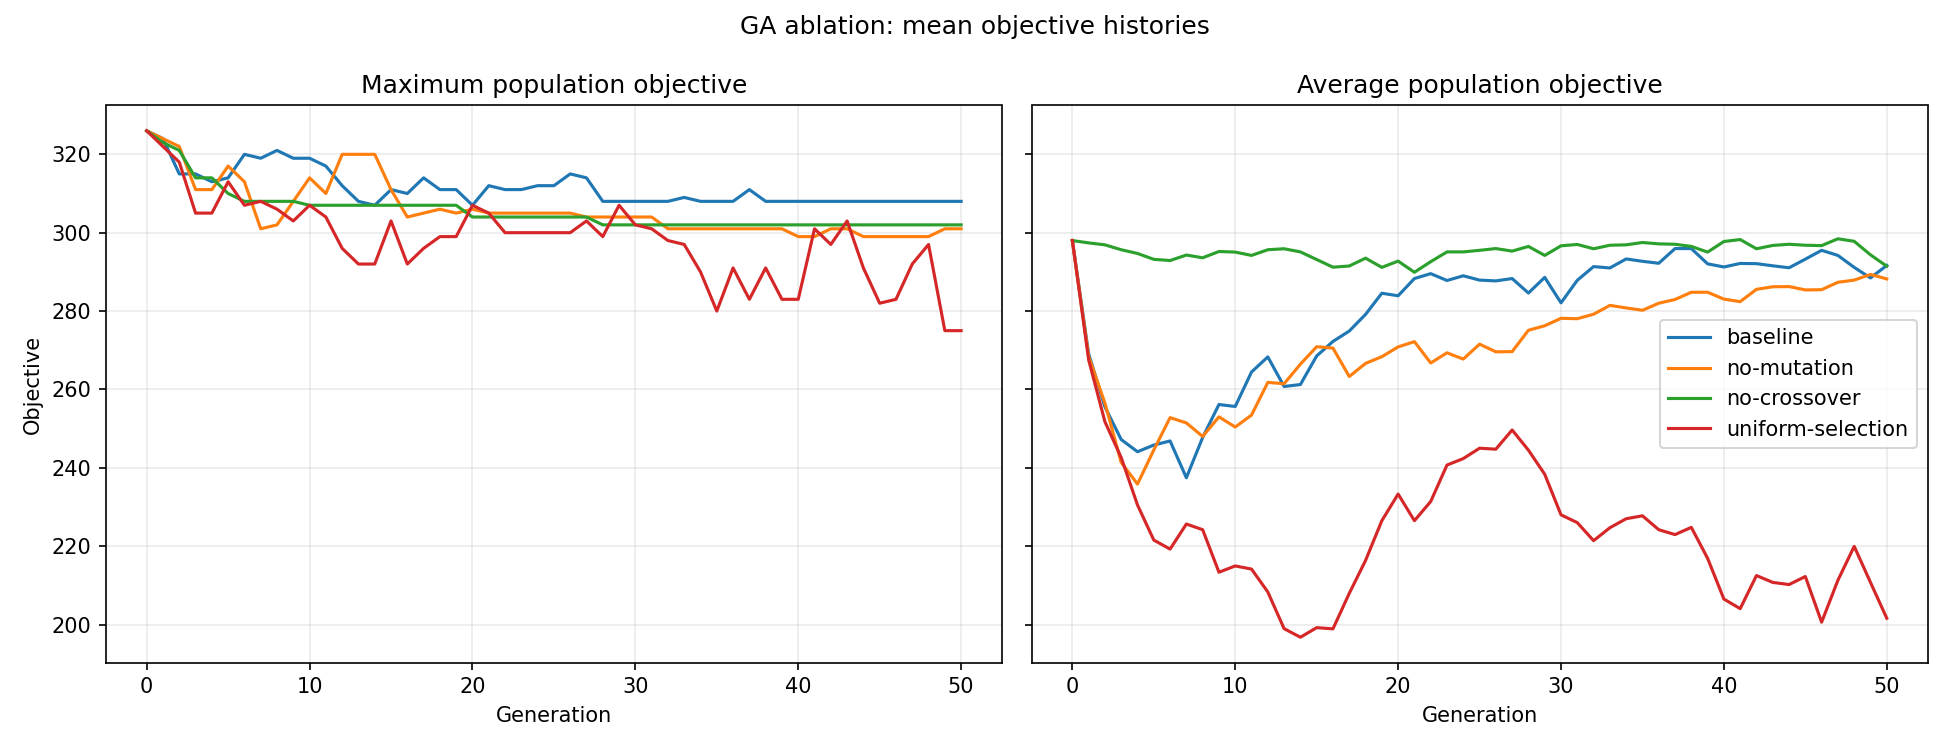
\includegraphics[width=0.85\textwidth]{figures/base/ga-ablation.png}
    \caption{Ablasi operator GA. Nilai maksimum dan rata-rata populasi per generasi}
\end{figure}

\begin{enumerate}
    \item \textbf{Dampak mutasi kecil pada percobaan ini.} Tanpa mutasi, rata-rata turun 1 poin dari 331 menjadi 330 dan seluruh \textit{run} berakhir pada 330. Baseline mencapai 335 pada seed 12. Lima seed belum cukup untuk memastikan bahwa mutasi menyebabkan perbedaan tersebut.
    \item \textbf{\textit{Crossover} dan seleksi \textit{roulette-wheel} tampak memberi manfaat kecil.} Tanpa \textit{crossover} atau dengan seleksi seragam, rata-rata turun 4--5 poin dan dua dari lima \textit{run} berakhir pada 320, sementara \textit{baseline} tidak pernah di bawah 330. Namun dengan lima \textit{seed} dan simpangan baku 5,5--6,7, selisih ini belum memenuhi syarat untuk disebut signifikan.
    \item \textbf{Biaya.} Menghilangkan \textit{crossover} memangkas durasi hampir separuh (0,196 dibanding 0,377 detik), yang menunjukkan bahwa \textit{crossover} beserta perbaikan (\textit{repair}) konflik adalah bagian termahal dari satu generasi.
\end{enumerate}

\subsection{Multi-Truck}

\subsubsection{Fixture Armada dan Protokol}

Eksperimen memakai 11 fixture sintetis yang mengikuti kategori pengujian sebelumnya. Setiap fixture mempertahankan paket dan spesifikasi truk sumber, lalu menyediakan dua truk identik. Perbedaan hasil terutama mencerminkan pembagian paket ke lebih dari satu truk, bukan perubahan ukuran atau kapasitas truk. Fixture mencakup kasus dasar, ruang dan kapasitas ketat, kasus tanpa pemuatan layak, serta tujuh kasus batas.

Setiap kombinasi fixture dan seed dijalankan dengan empat varian HC, SA, dan GA. Eksperimen memakai lima seed, yaitu 11 sampai 15, sehingga menghasilkan $11\times5\times6=330$ run. Untuk tiap fixture dan seed, seluruh metode menerima state awal yang sama. Seed pembentuk state awal diperoleh dengan XOR seed run dengan konstanta tetap $\texttt{0x5EED}$. Objective yang digunakan adalah \texttt{total\_value}.

Parameter mengikuti baseline runner armada. HC memakai 30 neighbor per iterasi, paling banyak 1000 iterasi, 100 sideways move, dan 10 restart. SA memakai 2000 iterasi, temperatur awal 100, laju pendinginan 0,995, dan patience 100 iterasi. GA memakai populasi 20, 40 generasi, dan laju mutasi 0,05. Anggaran komputasi ketiga algoritma tidak setara. Perbandingan ini menggambarkan perilaku konfigurasi yang diuji dan tidak menyimpulkan keunggulan algoritma pada biaya komputasi yang sama.

\subsubsection{State Awal sebagai Baseline}

State awal dianalisis sebelum hasil akhir dibandingkan. Untuk setiap fixture, ringkasan memakai satu state per seed, bukan satu salinan untuk setiap algoritma. Analisis mencatat validitas, nilai paket yang telah dimuat, jumlah paket termuat dan belum termuat, serta jumlah dan nilai paket pada masing-masing truk. Perubahan nilai dan jumlah paket pada akhir pencarian kemudian dihitung terhadap baseline ini.

\begin{table}[H]
    \centering
    \scriptsize
    \caption{Karakteristik state awal per fixture, rata-rata dan simpangan baku sampel dari lima seed}
    \label{tab:fleet-initial-states}
    \begin{tabular}{@{}lrrll@{}}
        \toprule
        Fixture                    & Nilai awal $\pm$ SD & Paket termuat & Truk 1 paket/nilai & Truk 2 paket/nilai \\
        \midrule
        \texttt{base}              & 568,0 $\pm$ 43,8    & 9,6           & 4,4 / 277,0        & 5,2 / 291,0        \\
        \texttt{tight-space}       & 355,0 $\pm$ 60,3    & 6,8           & 3,4 / 175,0        & 3,4 / 180,0        \\
        \texttt{tight-capacity}    & 300,0 $\pm$ 0,0     & 6,0           & 3,2 / 148,0        & 2,8 / 152,0        \\
        \texttt{infeasible}        & 0,0 $\pm$ 0,0       & 0,0           & 0,0 / 0,0          & 0,0 / 0,0          \\
        \texttt{equal-fitness}     & 60,0 $\pm$ 0,0      & 6,0           & 3,0 / 30,0         & 3,0 / 30,0         \\
        \texttt{exact-capacity}    & 125,0 $\pm$ 0,0     & 4,0           & 1,8 / 55,0         & 2,2 / 70,0         \\
        \texttt{fragile-support}   & 100,0 $\pm$ 0,0     & 3,0           & 1,4 / 36,0         & 1,6 / 64,0         \\
        \texttt{rotation-only}     & 100,0 $\pm$ 0,0     & 2,0           & 1,0 / 46,0         & 1,0 / 54,0         \\
        \texttt{single-package}    & 50,0 $\pm$ 0,0      & 1,0           & 0,4 / 20,0         & 0,6 / 30,0         \\
        \texttt{wall-touching}     & 100,0 $\pm$ 0,0     & 4,0           & 2,0 / 56,0         & 2,0 / 44,0         \\
        \texttt{zero-value-weight} & 70,0 $\pm$ 0,0      & 4,0           & 1,8 / 28,0         & 2,2 / 42,0         \\
        \bottomrule
    \end{tabular}
\end{table}

Pada \texttt{base}, state awal sudah memuat rata-rata 9,6 dari 10 paket dengan nilai 568. Dua seed yang nilainya 520 belum memuat paket P10. State awal \texttt{tight-space} lebih bervariasi, dengan nilai rata-rata 355 dan simpangan baku 60,3. Pada \texttt{tight-capacity}, seluruh seed mulai dari nilai 300 dan enam paket termuat. Pembagian muatan awal di dua truk relatif seimbang pada ketiga fixture tersebut. Karena state awal identik untuk semua metode pada seed yang sama, perbedaan hasil akhir bukan akibat perbedaan inisialisasi antaralgoritma.

\subsubsection{Hasil Lintas Fixture}

Tabel~\ref{tab:fleet-final-results} membandingkan rata-rata dan simpangan baku nilai akhir untuk setiap metode. Nilai awal pada Tabel~\ref{tab:fleet-initial-states} menjadi acuan untuk membaca perbaikan. Kasus \texttt{infeasible} hanya digunakan untuk memeriksa validitas keluaran, bukan untuk menentukan metode terbaik. Nilai maksimum yang muncul pada eksperimen merupakan hasil terbaik yang teramati dan tidak otomatis menjadi optimum global.

\begin{table}[H]
    \centering
    \scriptsize
    \caption{Nilai akhir rata-rata dan simpangan baku sampel dari lima seed, jumlah paket rata-rata dalam tanda kurung}
    \label{tab:fleet-final-results}
    \resizebox{\textwidth}{!}{%
        \begin{tabular}{@{}lrrrrrr@{}}
            \toprule
            Fixture                    & HC steepest            & HC sideways            & HC stochastic          & HC random restart      & SA                     & GA                     \\
            \midrule
            \texttt{base}              & 568,0 $\pm$ 43,8 (9,6) & 600,0 $\pm$ 0,0 (10,0) & 568,0 $\pm$ 43,8 (9,6) & 600,0 $\pm$ 0,0 (10,0) & 600,0 $\pm$ 0,0 (10,0) & 600,0 $\pm$ 0,0 (10,0) \\
            \texttt{tight-space}       & 366,0 $\pm$ 52,2 (7,0) & 423,0 $\pm$ 27,5 (7,8) & 366,0 $\pm$ 52,2 (7,0) & 442,0 $\pm$ 14,0 (8,0) & 464,0 $\pm$ 34,5 (8,2) & 472,0 $\pm$ 28,2 (8,2) \\
            \texttt{tight-capacity}    & 300,0 $\pm$ 0,0 (6,0)  & 300,0 $\pm$ 0,0 (6,0)  & 300,0 $\pm$ 0,0 (6,0)  & 300,0 $\pm$ 0,0 (6,0)  & 323,0 $\pm$ 11,5 (6,0) & 300,0 $\pm$ 0,0 (6,0)  \\
            \texttt{infeasible}        & 0,0 $\pm$ 0,0 (0,0)    & 0,0 $\pm$ 0,0 (0,0)    & 0,0 $\pm$ 0,0 (0,0)    & 0,0 $\pm$ 0,0 (0,0)    & 0,0 $\pm$ 0,0 (0,0)    & 0,0 $\pm$ 0,0 (0,0)    \\
            \texttt{equal-fitness}     & 60,0 $\pm$ 0,0 (6,0)   & 60,0 $\pm$ 0,0 (6,0)   & 60,0 $\pm$ 0,0 (6,0)   & 60,0 $\pm$ 0,0 (6,0)   & 60,0 $\pm$ 0,0 (6,0)   & 60,0 $\pm$ 0,0 (6,0)   \\
            \texttt{exact-capacity}    & 125,0 $\pm$ 0,0 (4,0)  & 125,0 $\pm$ 0,0 (4,0)  & 125,0 $\pm$ 0,0 (4,0)  & 125,0 $\pm$ 0,0 (4,0)  & 125,0 $\pm$ 0,0 (4,0)  & 125,0 $\pm$ 0,0 (4,0)  \\
            \texttt{fragile-support}   & 100,0 $\pm$ 0,0 (3,0)  & 100,0 $\pm$ 0,0 (3,0)  & 100,0 $\pm$ 0,0 (3,0)  & 100,0 $\pm$ 0,0 (3,0)  & 100,0 $\pm$ 0,0 (3,0)  & 100,0 $\pm$ 0,0 (3,0)  \\
            \texttt{rotation-only}     & 100,0 $\pm$ 0,0 (2,0)  & 100,0 $\pm$ 0,0 (2,0)  & 100,0 $\pm$ 0,0 (2,0)  & 100,0 $\pm$ 0,0 (2,0)  & 100,0 $\pm$ 0,0 (2,0)  & 100,0 $\pm$ 0,0 (2,0)  \\
            \texttt{single-package}    & 50,0 $\pm$ 0,0 (1,0)   & 50,0 $\pm$ 0,0 (1,0)   & 50,0 $\pm$ 0,0 (1,0)   & 50,0 $\pm$ 0,0 (1,0)   & 50,0 $\pm$ 0,0 (1,0)   & 50,0 $\pm$ 0,0 (1,0)   \\
            \texttt{wall-touching}     & 100,0 $\pm$ 0,0 (4,0)  & 100,0 $\pm$ 0,0 (4,0)  & 100,0 $\pm$ 0,0 (4,0)  & 100,0 $\pm$ 0,0 (4,0)  & 100,0 $\pm$ 0,0 (4,0)  & 100,0 $\pm$ 0,0 (4,0)  \\
            \texttt{zero-value-weight} & 70,0 $\pm$ 0,0 (4,0)   & 70,0 $\pm$ 0,0 (3,8)   & 70,0 $\pm$ 0,0 (4,0)   & 70,0 $\pm$ 0,0 (4,0)   & 70,0 $\pm$ 0,0 (4,0)   & 70,0 $\pm$ 0,0 (4,0)   \\
            \bottomrule
        \end{tabular}%
    }
\end{table}

\begin{figure}[H]
    \centering
    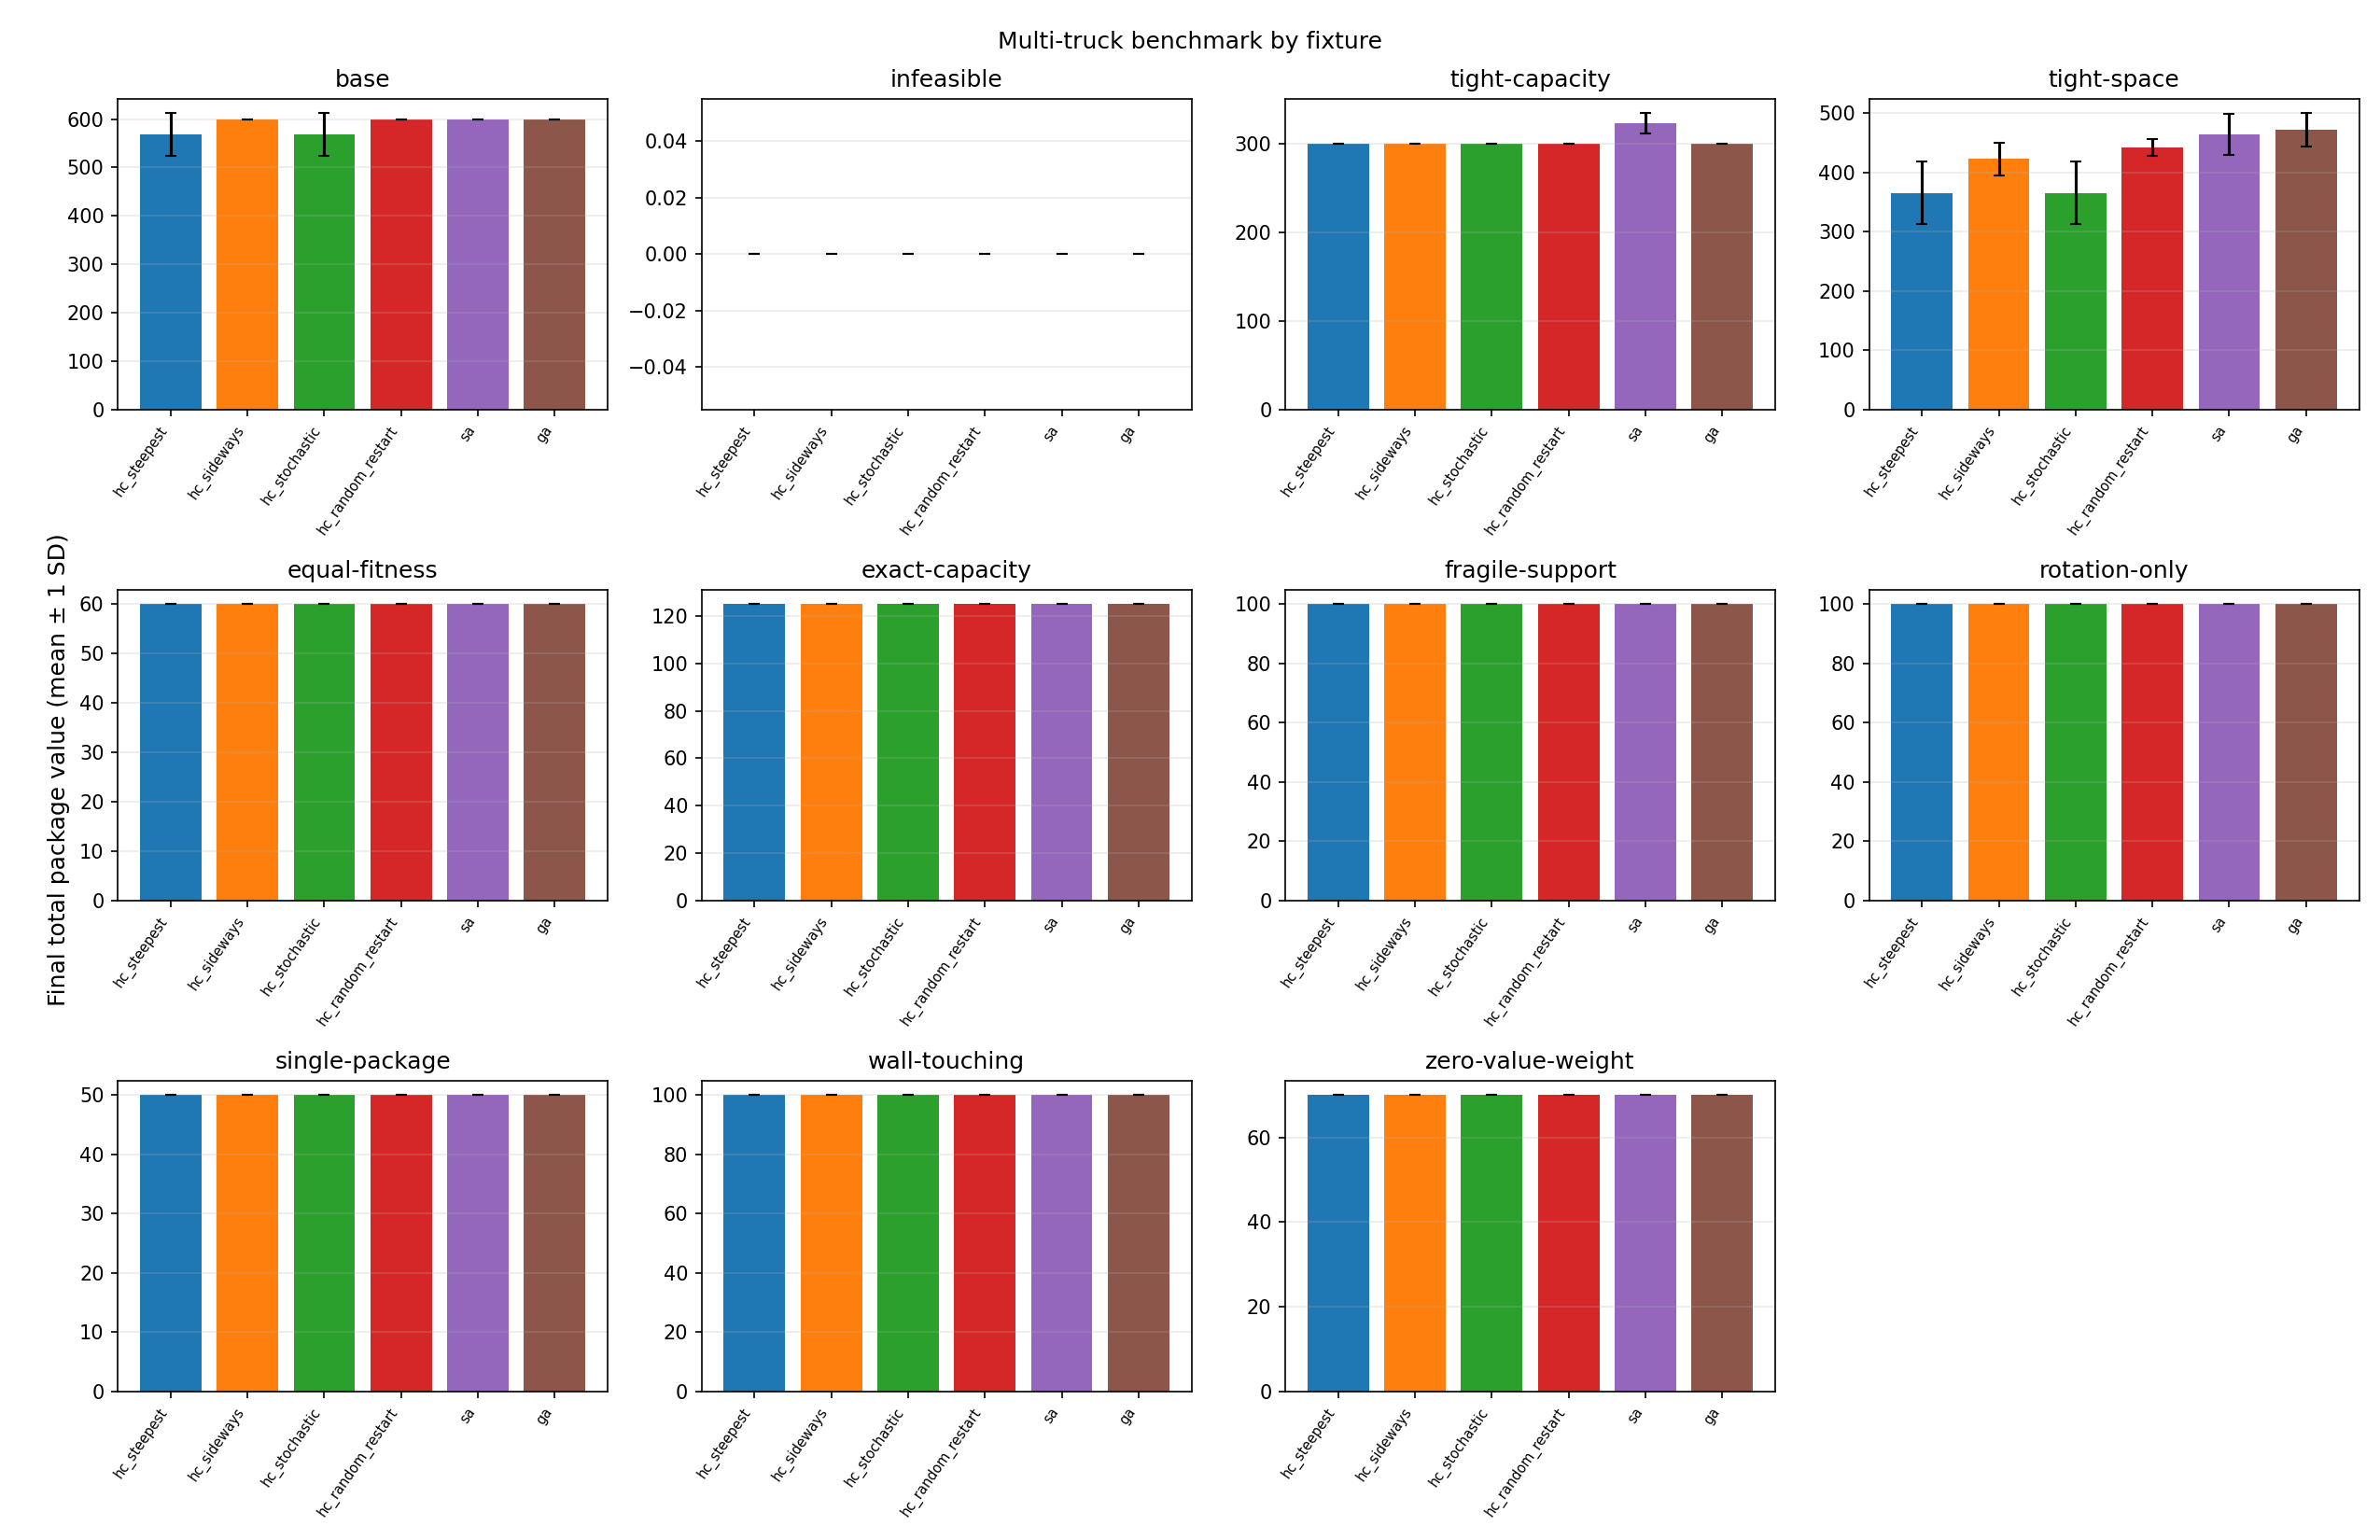
\includegraphics[width=0.6\textwidth]{figures/fleet-analysis/summary.png}
    \caption{Nilai akhir rata-rata per fixture dan metode dengan batang galat satu simpangan baku sampel}
    \label{fig:fleet-summary}
\end{figure}

Perbedaan antarmetode tampak terutama pada tiga fixture utama. Pada \texttt{base}, empat metode mencapai nilai 600 pada seluruh seed kecuali HC steepest dan HC stochastic, yang tidak memperbaiki dua state awal bernilai 520. Karena total nilai seluruh paket adalah 600 dan seluruh paket termuat pada hasil bernilai 600, nilai tersebut merupakan batas atas yang diketahui untuk fixture ini. HC sideways dan random restart, SA, serta GA mencapai batas itu pada kelima seed.

Pada \texttt{tight-space}, GA memiliki rata-rata tertinggi sebesar 472, disusul SA sebesar 464 dan HC random restart sebesar 442. GA dan SA sama-sama mencapai nilai terbaik teramati 520, tetapi sebaran hasil SA lebih besar. HC steepest dan stochastic menghasilkan rata-rata 366, sama dengan nilai awal rata-ratanya. Random restart memberi hasil lebih baik daripada tiga varian HC lain pada fixture ini, sementara sideways move membantu HC sideways memperbaiki sebagian seed.

\begin{figure}[H]
    \centering
    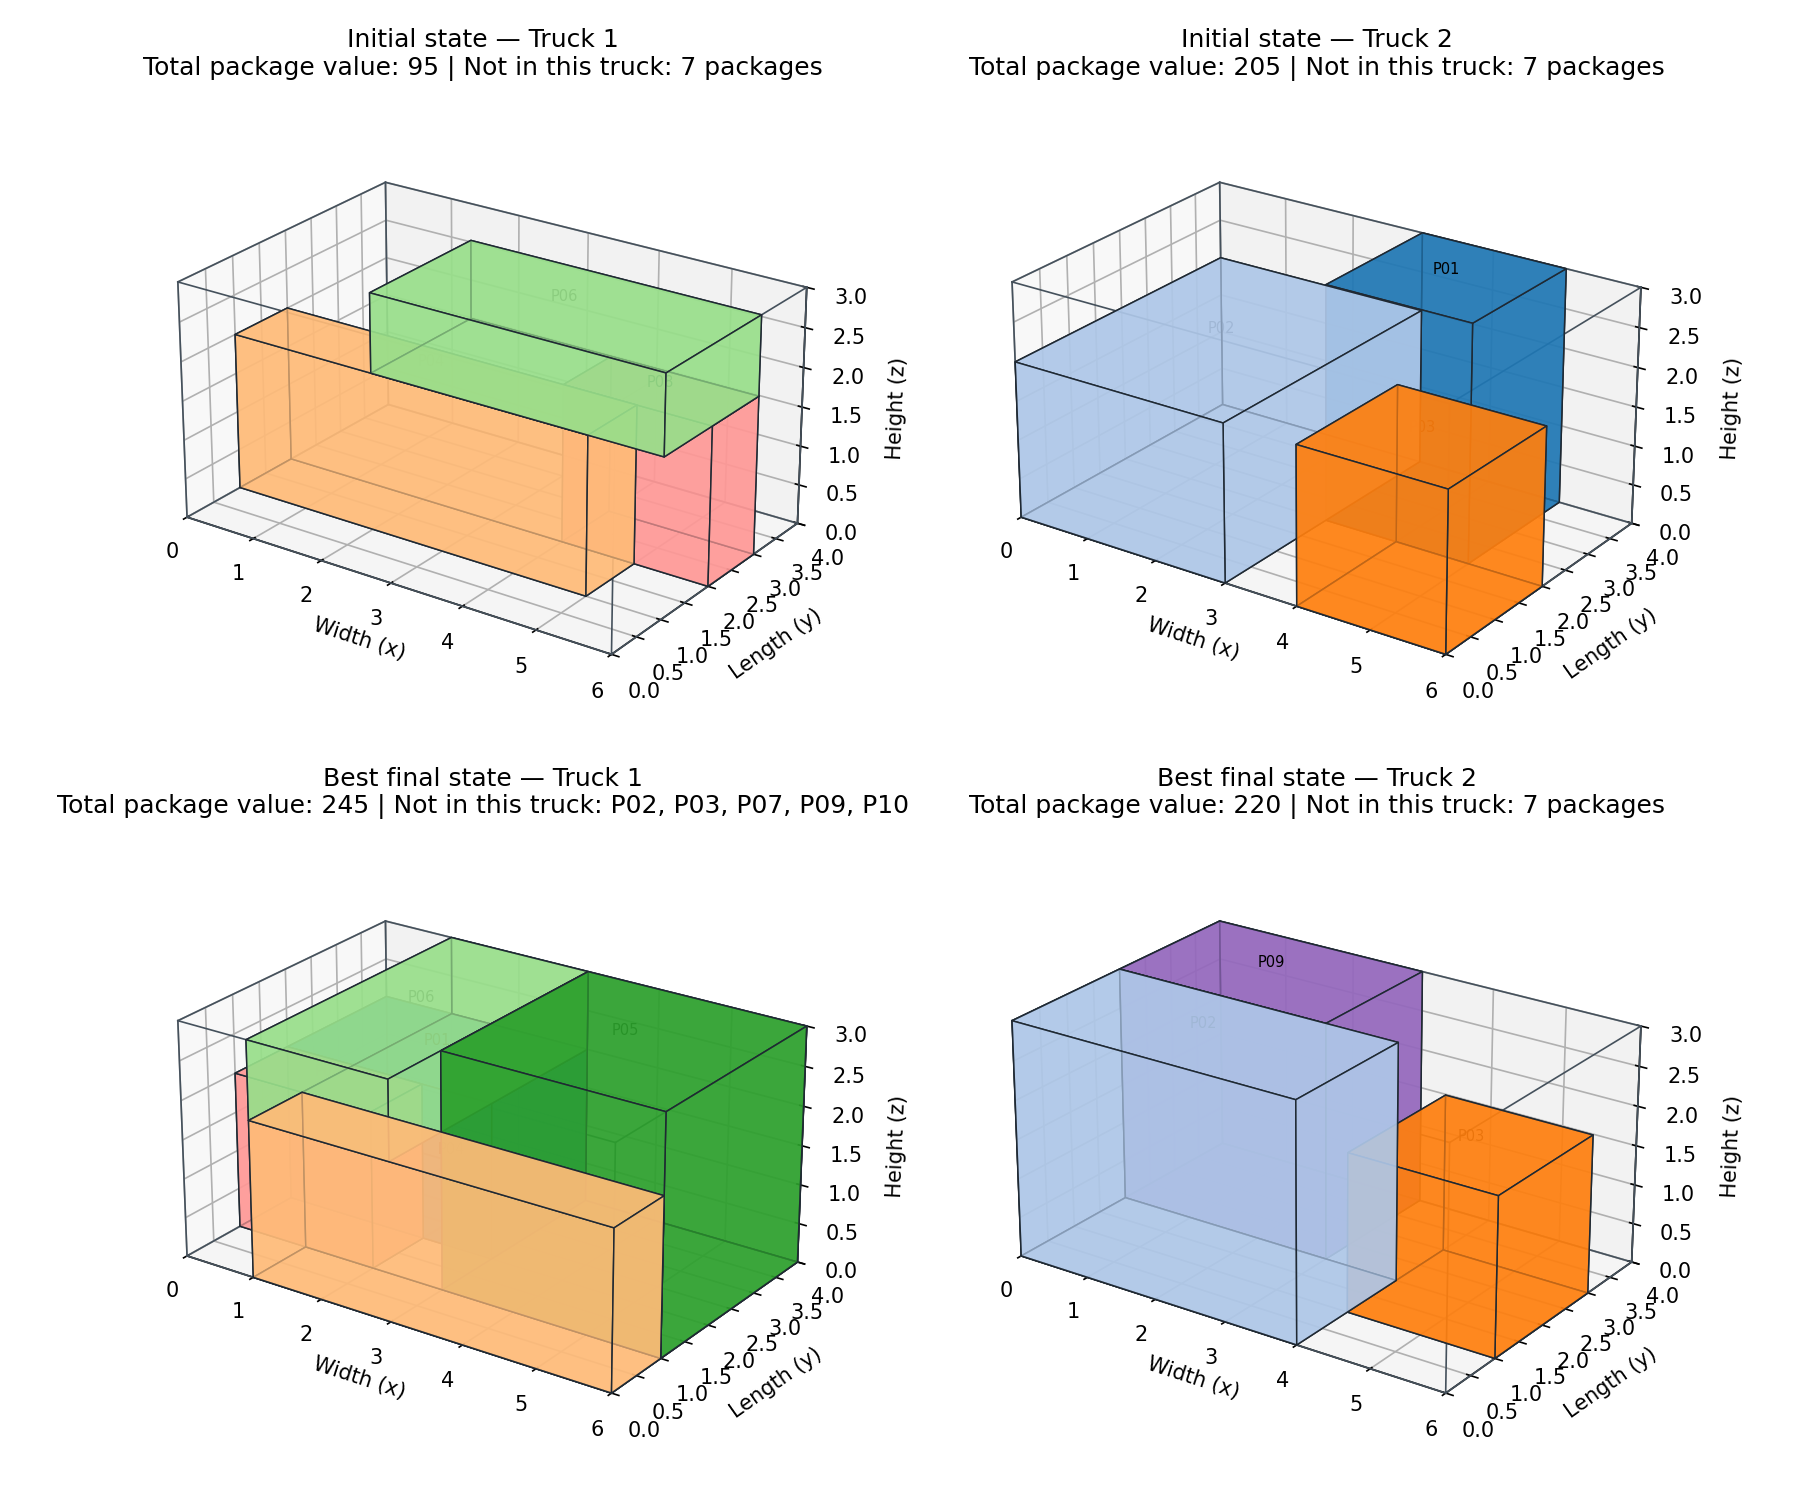
\includegraphics[width=0.9\textwidth]{figures/fleet-analysis/tight-space-ga.png}
    \caption{State awal dan state akhir GA pada fixture \texttt{tight-space} untuk seed 11}
    \label{fig:fleet-tight-space-state}
\end{figure}

Pada \texttt{tight-capacity}, nilai awal semua seed adalah 300. Empat varian HC dan GA tetap pada nilai itu, sedangkan SA mencapai rata-rata 323 dengan simpangan baku 11,5. Jumlah paket yang dimuat tetap enam pada seluruh hasil. Kenaikan nilai SA berasal dari perubahan paket yang dipilih, bukan dari bertambahnya jumlah paket. Pola ini sesuai dengan kemampuan SA menerima perpindahan yang sementara menurunkan nilai saat temperatur masih tinggi.

Tujuh fixture batas menghasilkan nilai akhir yang sama untuk seluruh metode dan seed. Kesamaan ini memperlihatkan bahwa kasus batas tersebut sudah terjangkau dari state awal yang dibangkitkan. Seluruh 55 state awal dan 330 state akhir lolos validasi. Pada \texttt{infeasible}, seluruh 30 run mengembalikan state kosong yang valid. Kasus tersebut memeriksa penanganan paket yang tidak dapat dimuat dan tidak masuk peringkat kualitas.

\subsubsection{Biaya Pencarian dan Karakteristik Algoritma}

Biaya pencarian berbeda walaupun semua metode memakai state awal berpasangan. Pada \texttt{base}, HC steepest menggunakan rata-rata 31 evaluasi objektif dan selesai dalam 0,031 detik. HC stochastic menggunakan 1001 evaluasi dan 1,211 detik. HC sideways memakai 3043 evaluasi dan 3,103 detik, sedangkan random restart menggunakan 359 evaluasi dan 0,535 detik. SA menggunakan 2001 evaluasi dengan durasi 2,225 detik. GA memakai 820 evaluasi, tetapi durasi 2,436 detik. Jumlah evaluasi saja tidak menggambarkan biaya operasi setiap algoritma, sehingga durasi dilaporkan bersamanya.

HC steepest dan stochastic berakhir pada nilai awal pada \texttt{base} untuk semua seed. Dua state awal bernilai 520 tidak membaik, sementara sideways dan random restart mencapai nilai 600 pada kedua seed tersebut. Sideways menghabiskan lebih banyak evaluasi untuk menerima gerakan setara. Random restart menemukan hasil yang sama dengan biaya evaluasi dan waktu lebih rendah pada konfigurasi ini. Pola ini tidak membuktikan bahwa random restart selalu lebih efisien pada instance lain.

SA memberi hasil tertinggi pada \texttt{tight-capacity}, dengan rata-rata 323 dibanding 300 untuk metode lain. Jumlah paketnya tetap enam. Pada kelima seed, paket yang dipilih SA berbeda dari state awal. Riwayat SA mencatat nilai state saat ini turun di bawah 300 pada semua seed, hingga serendah 115, sebelum menghasilkan state terbaik dengan nilai 310 sampai 335. Pada \texttt{tight-space}, SA mencapai rata-rata 464 dan GA 472. Kedua algoritma pernah menghasilkan nilai 520, sedangkan simpangan baku GA lebih kecil. Lima seed belum cukup untuk menyebut selisih tersebut signifikan.

GA mencapai rata-rata tertinggi pada \texttt{tight-space} dan 600 pada seluruh seed \texttt{base}. Namun, pada \texttt{tight-capacity}, nilai akhirnya tetap 300. Pada konfigurasi ini, populasi dan crossover belum memberi keuntungan pada semua struktur kasus. Biaya GA juga tidak berbanding lurus dengan banyak evaluasi. Pembentukan populasi, crossover, perbaikan konflik penempatan, dan validasi armada menambah pekerjaan di luar pemanggilan fungsi objektif.

Eksperimen ini memakai paket sintetis dan dua truk identik pada setiap fixture. Hasilnya belum mengukur armada heterogen atau armada dengan lebih dari dua truk. Lima seed memberi gambaran awal tentang variasi, tetapi tidak cukup untuk menguji signifikansi perbedaan. Parameter hanya memakai satu konfigurasi baseline per algoritma, dan biaya komputasinya berbeda. Batas atas nilai 600 diketahui untuk \texttt{base} dari jumlah nilai seluruh paket. Nilai tertinggi pada fixture lain hanya disebut sebagai hasil terbaik yang ditemukan, bukan optimum global. Run dapat diulang dengan \texttt{python -m src.experiments.fleet.run\_benchmark}. Catatan run, ringkasan, dan visualisasi tersimpan di \texttt{output/fleet-analysis/}.



\chapter{Kesimpulan dan Saran}
\section{Kesimpulan}

Tugas besar ini mengimplementasikan empat varian \textit{hill climbing}, \textit{simulated annealing}, dan \textit{genetic algorithm} untuk persoalan pemuatan paket tiga dimensi pada truk, di atas representasi \textit{state}, validator \textit{constraint}, dan fungsi \textit{neighbor} yang sama. Dari eksperimen pada Bab~4, diperoleh kesimpulan berikut.

\begin{enumerate}
    \item \textbf{Seluruh algoritma menghasilkan \textit{state} yang valid.} Seluruh 330 \textit{run} \textit{benchmark} satu truk dan 330 \textit{run} armada dua truk berakhir pada \textit{state} yang lolos validator. Pada \texttt{infeasible}, setiap \textit{run} mengembalikan \textit{state} kosong dengan nilai 0, dan kedelapan masukan tidak valid ditolak \textit{loader} sebelum pencarian dimulai. Representasi yang mengizinkan paket berada di luar truk membuat \textit{state} kosong selalu layak, sehingga pencarian tidak pernah kehilangan solusi yang valid.

    \item \textbf{\textit{Random restart}, SA, dan GA memberi kualitas yang setara dan lebih baik daripada varian \textit{hill climbing} lain.} Pada \texttt{base} dan \texttt{tight-capacity}, rata-rata ketiganya berada dalam sekitar 2\% dari optimum (335 dan 175) dan dalam sekitar 1\% satu sama lain, sedangkan \textit{steepest}, \textit{sideways}, dan \textit{stochastic} tertinggal 5--10\% dengan simpangan baku yang jauh lebih besar. Dengan lima \textit{seed}, selisih di antara ketiga algoritma terbaik lebih kecil daripada simpangan bakunya, sehingga tidak ada satu algoritma yang dapat dinyatakan paling unggul.

    \item \textbf{Dari sisi biaya, \textit{random restart} paling efisien pada konfigurasi yang diuji.} \textit{Random restart} mencapai kualitas yang sebanding dengan SA dan GA dengan 383 evaluasi objektif, dibandingkan 3001 pada SA dan 820 pada GA. \textit{Steepest} paling murah (43 evaluasi), tetapi hasilnya sangat bergantung pada \textit{state} awal. Durasi per evaluasi GA paling tinggi karena \textit{crossover}, perbaikan konflik, dan validasi turut dihitung, sehingga jumlah evaluasi saja bukan ukuran biaya yang adil antaralgoritma.

    \item \textbf{Kemampuan keluar dari \textit{local optimum} adalah pembeda utama.} \textit{State} awal \textit{seed} 12 pada \texttt{base} (bernilai 285) sudah merupakan \textit{local optimum} bagi \textit{steepest} dan \textit{sideways}. SA keluar darinya dengan menerima gerakan yang memburuk pada suhu tinggi (naik ke 320), sedangkan \textit{random restart} dan GA keluar dengan membangkitkan \textit{state} baru. Kasus \texttt{rotation-only} menunjukkan bahwa sebagian \textit{local optimum} berasal dari operator \textit{neighbor}: \textit{move} tidak pernah mengeluarkan paket dari truk dan \textit{swap} selalu memberi orientasi awal, sehingga dari beberapa \textit{state} tidak ada jalur ke \textit{state} yang lebih baik.

    \item \textbf{Kendala ruang lebih sulit daripada kendala kapasitas.} Pada \texttt{tight-space}, tidak ada algoritma yang rata-ratanya mencapai nilai terbaik teramati (300), padahal batas atas \textit{knapsack} berbasis berat adalah 335. Kesulitannya terletak pada penataan geometris, bukan pada pemilihan paket. Sebaliknya, \texttt{tight-capacity} hampir selalu diselesaikan secara optimal oleh \textit{random restart}, SA, dan GA.

    \item \textbf{Perbedaan antarvarian \textit{hill climbing} sesuai dengan mekanismenya.} \textit{Sideways move} membantu bila ada dataran yang dapat dilalui (misalnya pada \texttt{compact\_value} dan \texttt{tight-capacity}), tetapi 56--88 kali lebih lambat daripada \textit{steepest}, dan sekitar 18--24\% gerakannya tidak mengubah \textit{state}. \textit{Stochastic} hampir tidak lebih baik daripada \textit{steepest} meskipun sekitar 32 kali lebih lambat. Sebagian keunggulan \textit{random restart} berasal dari anggaran sebelas pendakian, bukan semata dari aturan penerimaannya.

    \item \textbf{Pada GA, ukuran populasi paling berpengaruh dan operatornya memberi manfaat kecil.} Menaikkan populasi dari 10 ke 40 menaikkan rata-rata dari 327 ke 333 dengan durasi sekitar lima kali, sedangkan menambah generasi di atas 40 tidak mengubah hasil. Laju mutasi 0,05 memberi rata-rata tertinggi; tanpa mutasi seluruh \textit{run} berhenti pada 330, dan laju 0,20 memperlebar sebaran. Ablasi menunjukkan bahwa menghilangkan \textit{crossover} atau mengganti \textit{roulette-wheel} dengan seleksi seragam menurunkan rata-rata 4--5 poin, sementara \textit{crossover} beserta \textit{repair} adalah bagian termahal dari satu generasi.

    \item \textbf{Pilihan \textit{objective function} menentukan solusi yang dicari.} \texttt{eta\_weighted\_value} memilih himpunan paket yang lebih mendesak dengan mengorbankan nilai total (misalnya SA pada \texttt{base}: nilai total turun dari 330 ke 305, skor ETA naik sekitar 24\%). \texttt{compact\_value} terutama mengubah penataan menjadi tumpukan yang lebih rendah tanpa mengurangi nilai total, dan gradien kecilnya membantu varian \textit{hill climbing} melewati dataran.

    \item \textbf{Pada armada dua truk, pola utamanya bertahan dengan perbedaan pada kasus ketat.} Pada \texttt{base} armada, semua metode kecuali \textit{steepest} dan \textit{stochastic} mencapai batas atas 600 pada kelima \textit{seed}. GA memberi rata-rata tertinggi pada \texttt{tight-space} (472), sedangkan SA adalah satu-satunya metode yang memperbaiki \texttt{tight-capacity} (rata-rata 323 dari nilai awal 300) dengan menukar paket yang dipilih.
\end{enumerate}

Secara keseluruhan, tidak ada satu algoritma yang unggul di semua kasus. \textit{Random restart hill climbing} memberi keseimbangan kualitas dan biaya terbaik pada \textit{instance} kecil yang diuji, SA paling mampu memperbaiki \textit{state} yang terjebak melalui gerakan memburuk, dan GA paling konsisten pada \texttt{base} serta paling kuat pada \texttt{tight-space} armada. Kesimpulan ini berlaku untuk \textit{instance} sintetis berukuran 1--10 paket, satu konfigurasi parameter per algoritma, dan tiga sampai lima \textit{seed}.

\section{Saran}

Berdasarkan hasil dan keterbatasan eksperimen, beberapa pengembangan berikut disarankan.

\begin{enumerate}
    \item \textbf{Memperbaiki operator \textit{neighbor}.} Operator \textit{move} sebaiknya dapat mengeluarkan paket dari truk, dan \textit{swap} sebaiknya mencoba seluruh orientasi paket yang masuk, bukan hanya orientasi awal. Perubahan ini menghilangkan \textit{local optimum} buatan seperti pada \texttt{rotation-only}. Selain itu, \texttt{random\_neighbor} sebaiknya tidak mengembalikan \textit{state} asal agar jatah \textit{sideways move} tidak terbuang untuk gerakan \textit{no-op}.

    \item \textbf{Menyamakan anggaran pencarian.} Perbandingan berikutnya sebaiknya memberi setiap algoritma jumlah evaluasi objektif atau batas waktu yang sama, termasuk menyamakan jumlah pendakian \textit{random restart} dengan anggaran algoritma lain. Dengan begitu, keunggulan suatu algoritma dapat dipisahkan dari besarnya anggaran yang diterimanya.

    \item \textbf{Menambah pengulangan dan uji statistik.} Jumlah \textit{seed} perlu ditambah, misalnya menjadi 30, dan perbandingan berpasangan diuji dengan uji nonparametrik seperti Wilcoxon \textit{signed-rank}. Dengan lima \textit{seed}, selisih antara \textit{random restart}, SA, dan GA belum dapat dibedakan dari \textit{noise}.

    \item \textbf{Menyetel parameter secara sistematis.} Suhu awal SA sebaiknya disesuaikan dengan skala \textit{objective}, misalnya dari rata-rata $|\Delta E|$ pada beberapa gerakan awal, karena skala \texttt{eta\_weighted\_value} jauh lebih kecil daripada \texttt{total\_value}. Sweep GA dapat diperluas ke kombinasi populasi dan laju mutasi serta dijalankan pada lebih dari satu \textit{instance}, dan SA dapat diberi kondisi berhenti dini agar tidak selalu menjalankan seluruh iterasi.

    \item \textbf{Memakai \textit{instance} yang lebih besar dan optimum yang diketahui.} \textit{Instance} dengan puluhan hingga ratusan paket diperlukan untuk menguji skalabilitas. Untuk kasus yang dibatasi ruang seperti \texttt{tight-space}, optimum sebenarnya dapat dihitung dengan solver eksak, misalnya formulasi \textit{integer programming}, agar kualitas solusi dapat diukur terhadap acuan, bukan hanya terhadap nilai terbaik yang ditemukan.

    \item \textbf{Mencoba pendekatan hibrida.} Hasil menunjukkan bahwa algoritma yang membangkitkan \textit{state} baru dan algoritma yang menerima gerakan memburuk sama-sama efektif keluar dari \textit{local optimum}. Kombinasi keduanya, seperti GA yang menjalankan \textit{hill climbing} singkat pada anak (\textit{memetic algorithm}) atau SA dengan \textit{restart}, layak diuji.

    \item \textbf{Memperluas eksperimen armada.} Eksperimen armada baru mencakup dua truk identik. Pengujian berikutnya dapat memakai truk dengan ukuran dan kapasitas berbeda serta lebih dari dua truk, dan menambahkan operator yang memindahkan paket antartruk secara langsung.

    \item \textbf{Menelusuri temuan yang belum dijelaskan.} Dua temuan belum diselidiki penyebabnya: SA dengan \texttt{compact\_value} sekitar 46\% lebih lambat pada \texttt{base}, dan \textit{random restart} kalah dari \textit{sideways} pada \texttt{eta\_weighted\_value}. Profil waktu dan eksperimen dengan lebih banyak \textit{seed} dapat memastikan apakah keduanya nyata atau hanya \textit{noise}.
\end{enumerate}


\chapter{Lampiran}
\section{Pembagian Tugas}

Pembagian tugas mengikuti pembagian yang tercatat pada \texttt{README.md} repositori.

\begin{table}[H]
\centering
\begin{tabular}{@{}p{4.6cm}p{2.3cm}p{8.4cm}@{}}
\toprule
Nama & NIM & Kontribusi \\
\midrule
Muhammad Aufar Rizqi Kusuma & 13524061 & Kontrak dan fondasi bersama (model, validator, \textit{neighbor}, \textit{SearchResult}), \textit{genetic algorithm}, serta bonus multi-truk \\
Arina Azka & 13524049 & \textit{Hill climbing} wajib beserta seluruh variannya (\textit{steepest}, \textit{sideways}, \textit{stochastic}, \textit{random restart}) sebagai bonus \\
Michael James Liman & 13524106 & \textit{Simulated annealing} wajib dan \textit{objective function} alternatif (\texttt{eta\_weighted\_value} dan \texttt{compact\_value}) sebagai bonus, termasuk penjalanan \textit{hill climbing} dan \textit{genetic algorithm} pada ketiga \textit{objective function} \\
\bottomrule
\end{tabular}
\caption{Pembagian tugas anggota kelompok Three Agents}
\end{table}

\section{Repositori GitHub}

Kode sumber, data eksperimen, visualisasi, dan sumber laporan ini tersedia pada repositori berikut.

\begin{center}
\url{https://github.com/parkuskus/IF3170_G11_ThreeAgents}
\end{center}

Struktur direktori utama repositori adalah sebagai berikut.

\begin{table}[H]
\centering
\begin{tabular}{@{}p{5.2cm}p{9.8cm}@{}}
\toprule
Lokasi & Isi \\
\midrule
\texttt{src/model.py}, \texttt{validation.py}, \texttt{neighbors.py}, \texttt{objectives.py} & Representasi \textit{state}, validator \textit{constraint}, pembangkit \textit{state} awal dan \textit{neighbor}, serta ketiga \textit{objective function} \\
\texttt{src/algorithms/} & Implementasi \textit{hill climbing}, \textit{simulated annealing}, dan \textit{genetic algorithm} \\
\texttt{src/experiments/} & Pelaksana eksperimen, termasuk perbandingan \textit{objective} dan ablasi GA \\
\texttt{src/visualization/} & Pembuat plot riwayat \textit{objective} dan tampilan 3D \textit{state} \\
\texttt{examples/} & Data \textit{instance}: \texttt{ga-hard.json} (8 paket) dan \texttt{ga-demo.json} (5 paket) \\
\texttt{output/} & Hasil \textit{run} (JSON) dan visualisasi untuk setiap algoritma dan \textit{objective} (\texttt{hc-hard}, \texttt{sa-hard}, \texttt{ga-hard}, dan padanan \texttt{-demo}) \\
\texttt{tests/} & Tes fondasi, algoritma, dan eksperimen \\
\bottomrule
\end{tabular}
\caption{Struktur repositori}
\end{table}

Dependensi dipasang dengan \texttt{python -m pip install -r requirements.txt} (Python 3.10 atau lebih baru), dan seluruh tes dijalankan dengan \texttt{python -m unittest discover -s tests -v} dari direktori utama repositori. Setiap \textit{run} mencatat \textit{seed} dan parameter pada berkas \texttt{result.json} sehingga hasil pada Bab Hasil Eksperimen dan Analisis dapat direproduksi.



\nocite{*}
\bibliography{dafpus}
\end{document}
